%------------------------ DOCUMENT CLASS ------------------------
\documentclass[12pt]{report}
% Set how paragraph changes are handled
\setlength{\parindent}{0ex} % 0 indent
\setlength{\parskip}{1ex} % skip one line

%---------------------------- PACKAGES ---------------------------
\usepackage[utf8]{inputenc}
\usepackage{graphicx}
\usepackage{verbatim}
\usepackage{amsmath}
\usepackage{hyperref}
\usepackage[inkscapelatex=false, inkscapepath=svgsubdir]{svg}
\usepackage{booktabs}
\usepackage{colortbl}
\usepackage{multirow}
\usepackage{float}
\usepackage{cancel}
\usepackage{titlesec}
\usepackage{geometry}
\usepackage[greek,english]{babel}
\usepackage{fancyhdr}
\usepackage{calc}
\usepackage{longtable}
\usepackage{subfig}
\usepackage{tabularx}
\usepackage{listings}
\usepackage{url}

%----------------------- CUSTOM COMMANDS -----------------------

% Increase header height
\setlength{\headheight}{14.5pt}

% Optionally adjust the top margin if you want to reduce space
\addtolength{\topmargin}{-2.5pt}

% Add functionality to \bmatrix so that it has a spacing input
\makeatletter
\renewcommand*\env@matrix[1][\arraystretch]{%
  \edef\arraystretch{#1}%
  \hskip -\arraycolsep
  \let\@ifnextchar\new@ifnextchar
  \array{*\c@MaxMatrixCols c}}
\makeatother


% Custom text style for chapter description
\newcommand{\chapterprecis}[1]{%
  \vfill 
  {\large\itshape #1} 
  \vspace{1.5in}
  \newpage
  }

% make sure that every section starts on a new page
\newcommand{\sectionbreak}{\clearpage}

%---------------------------  HEADERS ---------------------------
\fancyhf{}
\pagestyle{fancy}
\fancyhf{}
\fancyhead[L]{\thechapter\ - \leftmark}
\fancyhead[R]{\thesection\ - \rightmark}

\renewcommand{\chaptermark}[1]{\markboth{#1}{}}
\renewcommand{\sectionmark}[1]{\markright{#1}}

%---------------------------  FOOTERS ---------------------------
\fancyfoot[C]{\thepage} % Page number in the center of the footer
\setlength{\footskip}{90pt}

%------------------------  IMAGES PATHS -------------------------

\graphicspath{{images/}{images/Results/modal/}{images/Results/genetic algorithm/}{images/Results/Flutter/}{images/Results/Neural Net/}{images/Results/Powell/}}

%--------------------------- META DATA ---------------------------
\title{Aeroelastic Flutter Optimization of Wing Structures} 
\author{Xenodochidis Vasileios} 
\date{\today}


\bibliographystyle{plain}

%-------------------- MAIN DOCUMENT CONTROL ----------------------
\begin{document}
    \pagenumbering{roman}
    \newgeometry{top=0.5in, bottom=1in, left=1.5in, right=1.5in}
\begin{titlepage}


  % \begin{center}
  \begin{picture}(0,0)
    \put(-40,-525){\includegraphics[width=0.8\paperwidth]{mode4_17.386Hz.png}}
  \end{picture}
  
  % \end{center}


    \begin{figure}[H]
      \begin{center}
        \includegraphics[width=3cm]{LogoAUTH.png}
        \label{fig:cover_auth_logo}
      \end{center}
    \end{figure}
    
   \begin{center}
    
    \large Aristotle University of Thessaloniki\\
    \normalsize Department of Mechanical Engineering\\

    
    \vspace{0.7in}
    
    \LARGE\textbf{Aeroelastic Flutter Optimization of Wing Structures}
    
    \vspace{3in}
    
    \Large Xenodochidis Vasileios
    
    \end{center}
    
    \vfill

    \large

    \begin{tabular}{ccc}
        \textbf{Supervisors:} &Giagkopoulos Dimitrios, & Associate Proffesor.\\
        & Koutsoupakis Josef, & Ph.D. Candiadate

    \end{tabular}
    \vspace{1in}

    
    \centering
    \today
    
\end{titlepage}
\restoregeometry
    
    \begin{abstract}
    This thesis presents an aeroelastic analysis of a wing structure with
    the objective of optimizing its composite material to maximize flutter
    speed while minimizing mass. The study utilizes Altair's OptiStruct
    solver to compute flutter curves and assess the aeroelastic stability of
    the structure. Various optimization algorithms, implemented in Python,
    were employed to explore the design space and identify optimal
    configurations that balance structural mass and aeroelastic performance.
    Furthermore, a neural network model was developed to predict flutter
    speed based on key structural and material parameters, to see the
    potential that a surrogate model has in predicting the flutter speed.
    The results demonstrate significant improvements in both flutter speed
    and weight reduction, highlighting the potential of advanced
    optimization techniques and machine learning in aeroelastic design.
\end{abstract}

\selectlanguage{greek}
\begin{abstract}
    Η παρούσα διπλωματική εργασία παρουσιάζει μια αεροελαστική ανάλυση μιας
    πτέρυγας, με στόχο τη βελτιστοποίηση του πολυστρωματικoύ σύνθετου υλικού
    της για τη μεγιστοποίηση της ταχύτητας πτερυγισμού ελαχιστοποιώντας
    παράλληλα τη μάζα. Η μελέτη χρησιμοποιεί τον επιλυτή $OptiStruct$ της
    $Altair$ για να αξιολογήσει την αεροελαστική σταθερότητα της δομής.
    Διάφοροι αλγόριθμοι βελτιστοποίησης, που υλοποιήθηκαν στην $Python$,
    χρησιμοποιήθηκαν για να εξερευνήσουν το χώρο σχεδιασμού και να
    εντοπίσουν βέλτιστους συνδυασμούς παραμέτρων που παράγουν αποδεκτά
    χαρακτηριστικά πτερυγισμού ενώ ταυτόχρονα ελαχιστοποιούν τη μάζα της
    κατασκευής. Επιπλέον, αναπτύχθηκε ένα μοντέλο νευρωνικού δικτύου για την
    πρόβλεψη της ταχύτητας πτερυγισμού με βάση βασικές δομικές και υλικές
    παραμέτρους, για να αναδειχθούν οι δυνατότητες που έχει ένα υποκατάστατο
    μοντέλο στην πρόβλεψη της ταχύτητας πτερυγισμού. Τα αποτελέσματα
    δείχνουν σημαντικές βελτιώσεις τόσο στην ταχύτητα πτερυγισμού όσο και
    στη μείωση βάρους, τονίζοντας τις δυνατότητες των προηγμένων τεχνικών
    βελτιστοποίησης και της μηχανικής μάθησης στον αεροελαστικό σχεδιασμό.
\end{abstract}
    \selectlanguage{english}

    \pagestyle{plain}
    \tableofcontents
    
    \listoffigures    
    \listoftables

    \pagestyle{fancy}
    \clearpage
    \setcounter{page}{1}
    \pagenumbering{arabic}

    \setcounter{chapter}{0}
\chapter{Introduction}\label{introduction}

\chapterprecis{
The Introduction chapter describes the aim of the thesis. It also
defines the limits and scope of this work. Finally, it describes the
motivation behind this project.}

\section{Problem Statement}\label{problem-statement}

Aeroelasticity is a branch of physics and engineering which studies the
response of elastic bodies exposed to a fluid flow. The forces involved
in this interaction are inertial, elastic and aerodynamic. Aeroelastic
problems in engineering can be classified into two broad categories:
static aeroelasticity which deals with the steady state response, and
dynamic aeroelasticity dealing mainly with the body's vibrational
response.

The most common aeroelastic effects encountered by aircraft are:

\begin{itemize}
\item
  \emph{Aerodynamic Divergence}, where the deflection of lifting
  surfaces of an aircraft leads to additional lift that, in turn, leads
  to further deflection in the same direction, resulting in excessive
  stress or even leading to structural failure
\item
  \emph{Aeroelastic Control reversal,} where the forces generated by the
  control aileron (responsible for the roll control of an aircraft) are
  sufficient to twist the wing itself to such an extent that it changes
  the lift characteristics of the wing which makes the control surfaces
  ineffective or even produces the opposite of the expected result
\item
  \emph{Aeroelastic Flutter} is a dynamic instability of a structure
  that occurs due to the interaction of the fluid flow with the
  eigenmodes of the structure
\end{itemize}

In this thesis the flutter characteristics of a lifting surface will be
explored and tailored to specific requirements using optimization
techniques.

\section{Objective}\label{objective}

The objective of this project is to develop an understanding of the
flutter characteristics of a lifting surface made of a laminate
composite material and the methods used to computationally predict the
flutter region using Altair's Optistruct solver. Thereafter the effect
of several structural parameters is studied to determine their effect on
the flutter characteristics and the effectiveness of several
optimization techniques is tested to tailor the flutter characteristics
to a set of requirements using Python.

\section{Scope and Limitations}\label{scope-and-limitations}

The project will include:

\begin{itemize}
\item
  The study of composite materials and their implementation in the
  Optistruct solver
\item
  The study of the Vortex Lattice panel Method and how it is used during
  the Aerodynamic Flutter Analysis
\item
  The study of Aeroelastic Flutter Analysis on a theoretical basis by
  means of the governing equations of motion and on a computational
  basis by studying the implementation of theory into commercial
  solvers.
\item
  Investigation of the effect of composite material properties on the
  flutter characteristics
\item
  Investigation of different optimization techniques to manipulate the
  flutter characteristics including line search methods, genetic
  algorithms and Neural Networks
\end{itemize}

\section{Motivation}\label{motivation}

In the aerospace industry minimization of weight of structures is of
utmost importance, since it allows the increase of useful payload,
improves efficiency maneuverability and other control characteristics. A
consequence of structural weight minimization is the reduction of safety
margins in comparison to other engineering fields, thus the need for
more precise calculations arises to ensure safety.

As aerospace prototype testing costs are elevated, computer simulations
are used more and more and become ever more advanced with the ability to
study a wider range of phenomena. This project would help students and
researchers understand the basics of wing flutter instability and
provide insight into the optimization process for such structures. The
code developed in this project could also be extended and modified by
anyone tackling a similar project.

    \chapter{Θεωρητικό Υπόβαθρο}
\label{Ch:Theory}
\chapterprecis{Σε αυτό το κεφάλαιο παρουσιάζεται η βασική θεωρία που θα χρησιμοποιηθεί κατά τη διάρκεια αυτού του έργου. Το κεφάλαιο αυτό χωρίζεται σε τέσσερις κύριες ενότητες. Οι τρεις πρώτες ενότητες αφορούν στον υπολογισμό των χαρακτηριστικών του αεροελαστικού πτερυγισμού μιας ανυψωτικής επιφάνειας, ενώ η τέταρτη ενότητα παρουσιάζει τις διάφορες τεχνικές βελτιστοποίησης που θα χρησιμοποιηθούν.}

\section{Σύνθετα Πεπερασμένα Στοιχεία}\label{composite-finite-elements}

Η θεωρία πίσω από τα σύνθετα στοιχεία αναπτύσσεται σύμφωνα με τον \textlatin{E. Oñate}, στο έργο του \textlatin{``Structural Analysis with the Finite Element Method''} \cite{onate2013}, το οποίο παρέχει τις βασικές εξισώσεις και υποθέσεις που απαιτούνται για την ανάπτυξη 2Δ στοιχείων \textlatin{(shell elements)} τα οποία λαμβάνουν υπόψη την επίδραση των σύνθετων υλικών με πολλαπλά στρώματα. Το σύστημα συντεταγμένων που θα χρησιμοποιηθεί για την ανάλυση αυτών τον στοιχείων φαίνεται στο \autoref{fig:Composite element coordinate system}

\subsection{Πεδίο Μετατοπίσεων}\label{displacement-field}

Όταν μελετώνται τα σύνθετα στοιχεία πλακών με στρώματα, το κύριο πρόβλημα που προκύπτει είναι ότι, σε αντίθεση με τα ομογενή υλικά, σημεία που ανήκουν στο μέσο επίπεδο του στοιχείου μπορούν να μετακινηθούν ((εντός του επιπέδου)), κάτι που οδηγεί σε αξονικές δυνάμεις που δεν προκύπτουν σε ένα ομογενές υλικό. Για να ληφθεί υπόψη αυτό, εισάγουμε δύο αξονικές μετατοπίσεις $u_0(x,y)$ και $v_0(x,y)$ και έτσι η μετατόπιση οποιουδήποτε σημείου εντός της πλάκας μπορεί να υπολογιστεί ως εξής:

\foreignlanguage{english}{
\begin{subequations}
    \label{eq:disp_field}
    \begin{equation}
        u(x,y,z)=u_0(x,y) -z\theta_x (x,y)
    \end{equation}
    \begin{equation}
        v(x,y,z)=v_0(x,y) -z\theta_y (x,y)
    \end{equation}
    \begin{equation}
        w(x,y,z)=w_0 (x,y)
    \end{equation}
\end{subequations}
}

\begin{figure}[H]
  \centering
  \includesvg[width=\textwidth]{plate element axes.svg}
  \caption{Σύστημα συντεταγμένων σύνθετου στοιχείου}
  \label{fig:Composite element coordinate system}
\end{figure}



\subsection{Διανύσματα Παραμορφώσεων} \label{strain-vectors}

Η παραμόρφωση εντός της πλάκας μπορεί να υπολογιστεί ως εξής:

\begin{align}
    \label{eq:strain}
  \boldsymbol{\epsilon} &= 
  \begin{bmatrix}[1.2]
  \frac{\partial u}{\partial x} \\
  \frac{\partial v}{\partial y} \\
  \frac{\partial u}{\partial y} + \frac{\partial v}{\partial x} \\
  \frac{\partial u}{\partial z} + \frac{\partial w}{\partial x} \\
  \frac{\partial v}{\partial z} + \frac{\partial w}{\partial y}
  \end{bmatrix}
  \notag \\&=
  \begin{bmatrix}[1.2]
  \frac{\partial u_{0}}{\partial x} \\
  \frac{\partial v_{0}}{\partial y} \\
  \frac{\partial u_{0}}{\partial y} + \frac{\partial v_{0}}{\partial x} \\
  0 \\
  0
  \end{bmatrix}
  +
  \begin{bmatrix}[1.2]
  - z\frac{\partial\theta_{x}}{\partial x} \\
  - z\frac{\partial\theta_{y}}{\partial y} \\
  - z\left( \frac{\partial\theta_{x}}{\partial y} + \frac{\partial\theta_{y}}{\partial x} \right) \\
  \frac{\partial w_{0}}{\partial x} - \theta_{x} \\
  \frac{\partial w_{0}}{\partial y} - \theta_{y}
  \end{bmatrix}
  \notag \\&= 
  \begin{bmatrix}[1.2]
  \hat{\boldsymbol{\epsilon}}_{m} \\
  \mathbf{0}
  \end{bmatrix}
  +
  \begin{bmatrix}[1.2]
  - z \cdot \hat{\boldsymbol{\epsilon}}_{b} \\
  \hat{\boldsymbol{\epsilon}}_{s}
  \end{bmatrix}
  =
  \mathbf{S} \cdot \hat{\boldsymbol{\epsilon}}
\end{align}
  

Όπου:
$$
    \boldsymbol{\epsilon} =
    \begin{bmatrix}[1.2]
    \widehat{\boldsymbol{\epsilon}}_{m} \\
    \widehat{\boldsymbol{\epsilon}}_{b} \\
    \widehat{\boldsymbol{\epsilon}}_{s}
    \end{bmatrix}, \quad
    \widehat{\boldsymbol{\epsilon}}_{m} =
    \begin{bmatrix}[1.2]
    \frac{\partial u_{0}}{\partial x} \\
    \frac{\partial v_{0}}{\partial y} \\
    \frac{\partial u_{0}}{\partial y} + \frac{\partial v_{0}}{\partial x}
    \end{bmatrix}, \quad
    \widehat{\boldsymbol{\epsilon}}_{b} =
    \begin{bmatrix}[1.2]
    \frac{\partial\theta_{x}}{\partial x} \\
    \frac{\partial\theta_{y}}{\partial y} \\
    \frac{\partial\theta_{x}}{\partial y} + \frac{\partial\theta_{y}}{\partial x}
    \end{bmatrix}, \quad
    \widehat{\boldsymbol{\epsilon}}_{s} =
    \begin{bmatrix}[1.2]
    \frac{\partial w_{0}}{\partial x} - \theta_{x} \\
    \frac{\partial w_{0}}{\partial y} - \theta_{y}
    \end{bmatrix}
$$

είναι τα γενικευμένα διανύσματα τάσεων που οφείλονται σε παραμορφώσεις μεμβράνης ($m$), κάμψης ($b$) και εγκάρσιες  παραμορφώσεις ($s$).
\begin{equation}
    S =
    \begin{bmatrix}
    I_{3} & - z I_{3} & O_{2} \\[5pt]
    O_{3}^{T} & O_{2} & I_{2}
    \end{bmatrix}
\end{equation}

Όπου, $ I_{n} $ είναι ο $n \times n$ μοναδιαίος πίνακας, και

\[
O_{2} =
\begin{bmatrix}
0 & 0 \\
0 & 0
\end{bmatrix}, \quad
O_{3} =
\begin{bmatrix}
0 & 0 \\
0 & 0 \\
0 & 0
\end{bmatrix}
\]


από τη σχέση που προηγείται, μπορούμε να εξάγουμε τις εξής χρήσιμες εκφράσεις:

\begin{equation}
    \boldsymbol{\epsilon} = 
    \begin{bmatrix}
        \boldsymbol{\epsilon}_{\mathbf{p}} \\
        \boldsymbol{\epsilon}_{\mathbf{s}}
    \end{bmatrix}
\end{equation}

Όπου: 
$\boldsymbol{\epsilon}_{\mathbf{p}} = 
\begin{bmatrix}
\epsilon_{x} \\
\epsilon_{y} \\
\epsilon_{z}
\end{bmatrix} = \ {\hat{\boldsymbol{\epsilon}}}_{\mathbf{m}}\mathbf{-}z{\hat{\boldsymbol{\epsilon}}}_{\mathbf{b}}$
,\quad
$\boldsymbol{\epsilon}_{\mathbf{s}}=\begin{bmatrix}
\gamma_{xy} \\
\gamma_{yz}
\end{bmatrix}={\hat{\boldsymbol{\epsilon}}}_{\mathbf{s}}
$

\subsection{Σχέση Τάσεων - Παραμορφώσεων}\label{stress-strain-relationship}


Τώρα θα εξαχθεί η σχέση τάσεων-παραμορφώσεων σε μια σύνθετη πλάκα με στρώματα.

Θεωρούμε μια σύνθετη πλάκα με στρώματα που σχηματίζεται από την τοποθέτηση $n_{l}$ ορθότροπων στρώσεων όπως φαίνεται στο \autoref{fig:composite_layers}, οι οποίες ονομάζονται \textlatin{plies}, με άξονες ορθοτροπίας $L,T,z$ και ισοτροπία στον άξονα $L$ (στο επίπεδο $Tz$). Ο άξονας $L$ είναι παράλληλος προς την κατεύθυνση των επιμήκων ινών του σύνθετου υλικού.

Θα υποτεθεί ότι:

\begin{itemize}
\item
  Κάθε στρώση ($k$) ορίζεται από το επίπεδο $z = z_{k}$ και $z = z_{k + 1}$ με $z_{k} \leq z \leq z_{k + 1}$.
\item
  Οι άξονες ορθοτροπίας $L$ και $T$ μπορεί να μεταβάλλονται για κάθε στρώση και εκπροσωπούνται από τη γωνία $\beta_{i}$, η οποία ορίζεται ως η γωνία μεταξύ του \textlatin{global} άξονα $x$ και του άξονα $L_{i}$ της $i$-οστής στρώσης.
\item
  Κάθε στρώση ικανοποιεί την υπόθεση για την παραμόρφωση στο επίπεδο, δηλαδή $\sigma_{z} = 0$ και ο άξονας $z$ είναι ο άξονας ορθοτροπίας που είναι κοινός για όλες τις στρώσεις.
\item
Το πεδίο μετατοπίσεων είναι συνεχές μεταξύ των στρώσεων και ικανοποιεί την εξίσωση \eqref{eq:disp_field}.
\end{itemize}

\begin{figure}[h]
    \centering
    \includegraphics[width=0.7\textwidth]{"composite layers definition.png"}
    \caption{Ορισμός στρωμάτων σε \textlatin{composite laminated plate \cite{onate2013}}}
    \label{fig:composite_layers}
\end{figure}


Οι παραδοχές που αναφέρθηκαν παραπάνω, μας επιτρέπουν να εκφράσουμε τη σχέση μεταξύ των τάσεων εντός του επιπέδου $\sigma_{x},\ \sigma_{y},\ \tau_{xy}$ και των εγκάρσιων διατμητικών παραμορφώσεων $\tau_{xz},\tau_{yz}$ με τις αντίστοιχες παραμορφώσεις για κάθε στρώση $k$ ως εξής:
\begin{equation}
    \boldsymbol{\sigma}_{\mathbf{p}} =
    \begin{bmatrix}
        \sigma_{x} \\
        \sigma_{y} \\
        \tau_{xy}
    \end{bmatrix} \\
    = \mathbf{D_p}
    \begin{bmatrix}
        \epsilon_{x} \\
        \epsilon_{y} \\
        \gamma_{xy}
    \end{bmatrix} \\
    = \mathbf{D_p} \boldsymbol{\epsilon}_{p}
\end{equation}
    

\begin{equation}
    \boldsymbol{\sigma}_{\mathbf{s}} = \begin{bmatrix}
    \tau_{xz} \\
    \tau_{yz}
    \end{bmatrix} \\
    = \mathbf{D}_{\mathbf{s}} \begin{bmatrix}
    \gamma_{xz} \\
    \gamma_{yz}
    \end{bmatrix} \\
    = \mathbf{D}_{\mathbf{s}} \boldsymbol{\epsilon}_{s}
    \end{equation}
    

Και τέλος,
\begin{equation}
\begin{array}{r}
\boldsymbol{\sigma}=\begin{bmatrix}
\boldsymbol{\sigma_p} \\
\boldsymbol{\sigma_s}
\end{bmatrix}=\begin{bmatrix}
\mathbf{D}_{\mathbf{p}} & \mathbf{0} \\
\mathbf{0} & \mathbf{D_s}
\end{bmatrix}\mathbf{\cdot}\begin{bmatrix}
\boldsymbol{\epsilon_{p}} \\
\boldsymbol{\epsilon}_{\mathbf{s}}
\end{bmatrix}=\boldsymbol{D\epsilon}
\end{array}
\end{equation}



Τα καταστατικά μητρώα (\textlatin{constitutive matrices}) $\mathbf{D_{p}, D_{s}}$ είναι συμμετρικά και τα στοιχεία τους εξαρτώνται από τις πέντε ανεξάρτητες ιδιότητες του υλικού καθώς και από τη γωνία $\beta_{k}$. Ο υπολογισμός των προαναφερθέντων μητρώων ξεκινά εκφράζοντας τις σχέσεις τάσεων-παραμορφώσεων στους άξονες ορθοτροπίας $L, T, z$.

\begin{equation}    
\begin{array}{r}
\sigma_{1} = \mathbf{D}_{\mathbf{1}}\epsilon_{1},\ \ \sigma_{2} = \mathbf{D}_{\mathbf{2}}\epsilon_{2}
\end{array}
\end{equation}

Όπου:
\begin{center}

$\sigma_{1} = \begin{bmatrix}
\sigma_{L} \\
\sigma_{T} \\
\tau_{LT}
\end{bmatrix},\ \ \epsilon_{1} = \begin{bmatrix}
\epsilon_{L} \\
\epsilon_{T} \\
\gamma_{LT}
\end{bmatrix},\ \ \mathbf{D}_{\mathbf{1}}=\begin{bmatrix}
D_{LL} & D_{LT} & 0 \\
\  & D_{TT} & 0 \\
Sym. & \  & G_{LT}
\end{bmatrix}$

\vspace{10pt}
$\sigma_{2} = \begin{bmatrix}
\tau_{Lz} \\
\tau_{Tz}
\end{bmatrix},\ \ \epsilon_{2} = \begin{bmatrix}
\gamma_{Lz} \\
\gamma_{Tz}
\end{bmatrix},\ \ \mathbf{D}_{\mathbf{2}}=\begin{bmatrix}
G_{Lz} & 0 \\
0 & G_{Tz}
\end{bmatrix}$
\end{center}

\[D_{LL} = \frac{E_{L}}{a},\ \ D_{TT} = \frac{E_{T}}{a},\ \ a = 1 - \nu_{LT}\nu_{TL},\ \ D_{LT} = \frac{E_{T}\ \nu_{LT}}{a}\]

Οι πέντε πιο συχνά χρησιμοποιούμενες ανεξάρτητες παράμετροι του υλικού είναι:

\[E_{L},\ \ E_{T},\ \ \nu_{LT}\left( or\ \nu_{TL} = \frac{E_{T}}{E_{L}}\nu_{LT} \right),\ \ G_{Lz} = G_{LT},\ \ G_{Tz}\]

Τέλος, η σχέση μεταξύ των μητρώων $D_{1},\ D_{2}$ και $D_{p},\ D_{s}$ μπορεί να εκφραστεί ως ένα απλό γινόμενο μητρώων με τους πίνακες μετασχηματιστισμού $T_{1}$ και $T_{2}$ ως εξής:

\begin{equation}    
\mathbf{D_{p}} = T_{1}^{T} \cdot \mathbf{D_{1}} \cdot T_{1},\ \ \mathbf{D_{s}} = T_{2}^{T} \cdot \mathbf{D_{2}} \cdot T_{2}
\end{equation}

Όπου:

\[T_{1} = \begin{bmatrix}
\cos^{2}\left( \beta_{k} \right) & \sin^{2}\left( \beta_{k} \right) & \cos\left( \beta_{k} \right)sin(\beta_{k}) \\
\sin^{2}\left( \beta_{k} \right) & \cos^{2}\left( \beta_{k} \right) & - \cos\left( \beta_{k} \right)sin(\beta_{k}) \\
 - {2cos}{\left( \beta_{k} \right)\sin\left( \beta_{k} \right)} & {2cos}{\left( \beta_{k} \right)\sin\left( \beta_{k} \right)} & \cos^{2}\left( \beta_{k} \right) - \sin^{2}\left( \beta_{k} \right)
\end{bmatrix}\]

\[T_{2} = \begin{bmatrix}
\cos\left( \beta_{k} \right) & \sin\left( \beta_{k} \right) \\
 - \sin\left( \beta_{k} \right) & \cos\left( \beta_{k} \right)
\end{bmatrix}\]


\subsection{Γενικευμένο Καταστατικό Μητρώο}
\label{generalized-constitutive-matrix}
\begin{equation}
{\hat{\boldsymbol{\sigma}}}_{m} = \begin{bmatrix}
N_{x} \\
N_{y} \\
N_{xy}
\end{bmatrix} = \int_{- \frac{t}{2}}^{\frac{t}{2}}{\boldsymbol{\sigma}_{\mathbf{p}}dz},\ \ membrane\ forces
\end{equation}

\begin{equation}    
{\hat{\boldsymbol{\sigma}}}_{b} = \begin{bmatrix}
M_x \\
M_y \\
M_{xy}
\end{bmatrix} = - \int_{- \frac{t}{2}}^{\frac{t}{2}}{z\boldsymbol{\sigma}_{\mathbf{p}}dz},\ \ Bending\ moments
\end{equation}

\begin{equation}
    \hat{\boldsymbol{\sigma}}_{s} = \begin{bmatrix}
    Q_x \\
    Q_y
    \end{bmatrix} = \int_{-\frac{t}{2}}^{\frac{t}{2}} z \boldsymbol{\sigma}_{\mathbf{s}} \, dz \quad \ Transverse \ shear \ forces
\end{equation}
    
\begin{align}
    \hat{\boldsymbol{\sigma}}_{m} &= {\hat{\mathbf{D}}}_{m}{\hat{\epsilon}}_{m} + {\hat{\mathbf{D}}}_{mb}{\hat{\epsilon}}_{b} \\
    \hat{\boldsymbol{\sigma}}_{b} &= {\hat{\mathbf{D}}}_{mb}{\hat{\epsilon}}_{m} + {\hat{\mathbf{D}}}_{b}{\hat{\epsilon}}_{b} \\
    \hat{\boldsymbol{\sigma}}_{s} &= {\hat{\mathbf{D}}}_{s}{\hat{\epsilon}}_{s}
\end{align}
    

Όπου:
\begin{equation}
    \label{eq:Dm}
\begin{array}{r}
{\hat{\mathbf{D}}}_{m} = \int_{- t/2}^{t/2}{\mathbf{D}_{p}dz} 
\end{array}
\end{equation}


\begin{equation} 
    \label{eq:Dmb}  
\begin{array}{r}
{\hat{\mathbf{D}}}_{mb} = \int_{- t/2}^{t/2}{z\mathbf{D}_{p}dz}
\end{array}
\end{equation}

\begin{equation}
    \label{eq:Db}
\begin{array}{r}
{\hat{\mathbf{D}}}_{b} = \int_{- t/2}^{t/2}{z^{2}\mathbf{D}_{p}dz}\
\end{array}
\end{equation}


\begin{equation}
    \label{eq:Dshear}    
\hat{\mathbf{D}}_{\mathbf{s}} =
\begin{bmatrix}
k_{11} \overline{D}_{s_{11}} & k_{12} \overline{D}_{s_{12}} \\
\text{Συμ.} & k_{22} \overline{D}_{s_{22}}
\end{bmatrix}, \quad
\text{με} \quad
\overline{D}_{s_{ij}} = \int_{- \frac{t}{2}}^{\frac{t}{2}} D_{s_{ij}} \, dz
\end{equation}




Στην εξίσωση \ref{eq:Dshear}, οι όροι $k_{ij}$ ονομάζονται συντελεστές διόρθωσης για τη διάτμηση.

Τα ολοκληρώματα στις εξισώσεις \ref{eq:Dm} - \ref{eq:Dshear} μπορούν να εκφραστούν ως πεπερασμένο άθροισμα όταν η σύνθετη πλάκα \textlatin{laminate} αποτελείται από $n_{l}$ ορθότροπες στρώσεις. Για σύνθετες πλάκες, όπου οι άξονες $x$ και $y$ ταυτίζονται με τους άξονες ορθοτροπίας για όλες τις στρώσεις, ο πίνακας ${\hat{\mathbf{D}}}{\mathbf{s}}$ είναι διαγώνιος και μόνο οι όροι $k{11}$ και $k_{22}$ χρειάζεται να υπολογιστούν.
\\
Ο απλούστερος τρόπος υπολογισμού των συντελεστών διόρθωσης διάτμησης είναι η υπόθεση κυλινδρικής κάμψης. Αυτό σημαίνει ότι:
\begin{equation}
\frac{\partial\sigma_{x}}{\partial x} + \frac{\partial\tau_{xz}}{\partial z} = 0\ 
\end{equation}

Υποθέτοντας περαιτέρω μια σταθερή κατανομή της εγκάρσιας διατμητικής τάσης στην κατεύθυνση του πάχους και μετά από μερικούς υπολογισμούς, τελικά προκύπτει:

\begin{equation}
k_{11} = {\hat{D}}_{b_{11}}^{2}\left\lbrack {\overline{G}}_{xz}\int_{- t\text{/}2}^{t\text{/}2}{\frac{g_{1}^{2}(z)}{G_{xz}}dz} \right\rbrack^{- 1}
\end{equation}

\begin{equation}
k_{22} = {\hat{D}}_{b_{22}}^{2}\left\lbrack {\overline{G}}_{yz}\int_{- t\text{/}2}^{t\text{/}2}{\frac{g_{2}^{2}(z)}{G_{yz}}dz} \right\rbrack^{- 1}
\end{equation}

Όπου:

\begin{align*}
  g_{1(z)} &= \int_{- t\text{/}2}^{z}{zD_{p_{11}}dz}\\
  g_{2(z)} &= \int_{- t\text{/}2}^{z}{zD_{p_{22}}dz}\\
  {\overline{G}}_{xz} &= \int_{- t\text{/}2}^{t\text{/}2}G_{xz}dz\\
  {\overline{G}}_{yz} &= \int_{- t\text{/}2}^{t\text{/}2}G_{yz}dz
\end{align*}


Οι εξισώσεις \eqref{eq:Dm} έως \eqref{eq:Dshear} μπορούν να εκφραστούν ως πεπερασμένο άθροισμα όταν το σύνθετο \textlatin{laminate} αποτελείται από $n_{l}$ ορθότροπες στρώσεις, εντός των οποίων οι ιδιότητες του υλικού είναι σταθερές.

\begin{equation}
{\hat{\mathbf{D}}}_{m} = \sum_{k = 1}^{n_{l}}{t_{k}\mathbf{D}_{pk}}
\end{equation}

\begin{equation}
{\hat{\mathbf{D}}}_{mb} = - \sum_{k = 1}^{n_{l}}{t_{k}{\overline{z_{k}}\mathbf{D}}_{pk}}
\end{equation}

\begin{equation}
    \hat{\mathbf{D}}_{b} = \sum_{k = 1}^{n_{l}} \frac{1}{3} \left( \overline{z}_{k + 1}^{3} - z_{k}^{3} \right) \mathbf{D}_{pk}
\end{equation}


\begin{equation}
\ {\hat{\mathbf{D}}}_{\mathbf{s}}=\begin{bmatrix}
{\widetilde{k}}_{11}\ \sum_{k = 1}^{n_{l}}{t_{k}\mathbf{D}_{sk_{11}}}\ \ \  & 0 \\
0 & {\widetilde{k}}_{22}\sum_{k = 1}^{n_{l}}{t_{k}\mathbf{D}_{sk_{22}}}
\end{bmatrix}
\end{equation}

Όπου:

\[t_{k} = z_{k + 1} - z_{k},\ \ {\overline{z}}_{k} = \frac{1}{2}\left( z_{k + 1} + z_{k} \right)\]

\[{\widetilde{k}}_{ii} = {\hat{\mathbf{D}}}_{b_{ii}} \cdot \left\lbrack \sum_{k = 1}^{n_{l}}{t_{k}G_{xz}} \cdot \sum_{k = 1}^{n_{l}}\left( \frac{\sum_{l = 1}^{k}\left( t_{k}{\overline{z}}_{k}\mathbf{D}_{p_{{ii}_{l}}} \right)}{G_{xz_{k}}}t_{k} \right) \right\rbrack,\ \ i = 1,\ 2\]

\subsection{Διακριτοποιημένη τάση και παραμόρφωση - Συναρτήσεις Μορφής}\label{discretized-stress-and-strain---shape-functions}


Οι μετατοπίσεις εντός ενός σύνθετου τετραγωνικού στοιχείου τεσσάρων κόμβων μπορούν να εκφραστούν μέσω των συναρτήσεων μορφής.

\begin{equation}
\mathbf{u} = \begin{bmatrix}
u \\
v \\
w \\
\theta_{x} \\
\theta_{y}
\end{bmatrix} = \sum_{i = 1}^{4}{N_{i}a_{i}} = \mathbf{N \cdot}\vec{\mathbf{a}}
\end{equation}

Όπου:

\[
\mathbf{N} = \begin{bmatrix} \mathbf{N_1} \mid \mathbf{N_2} \mid \mathbf{N_3} \mid \mathbf{N_4} \end{bmatrix}
\]

\[
\mathbf{N_i} =  
  \begin{bmatrix}
      N_i & 0 & 0 & 0 & 0  \\
      0 & N_i & 0 & 0 & 0  \\
      0 & 0 & N_i & 0 & 0  \\
      0 & 0 & 0 & N_i & 0  \\
      0 & 0 & 0 & 0 & N_i 
  \end{bmatrix}, \quad for \ i \in \{1,2,3,4\}
\]



\[\vec{\mathbf{a}}=\begin{bmatrix}
{\vec{\mathbf{a}}}_{\mathbf{1}} \\
{\vec{\mathbf{a}}}_{\mathbf{2}} \\
{\vec{\mathbf{a}}}_{\mathbf{3}} \\
{\vec{\mathbf{a}}}_{\mathbf{4}}
\end{bmatrix}=\begin{bmatrix}
u_{1} \\
v_{1} \\
w_{1} \\
\theta_{x_{1}} \\
\theta_{y_{1}} \\
u_{2} \\
v_{2} \\
w_{2} \\
\theta_{x_{2}} \\
\theta_{y_{2}} \\
u_{3} \\
v_{3} \\
w_{3} \\
\theta_{x_{3}} \\
\theta_{y_{3}} \\
u_{4} \\
v_{4} \\
w_{4} \\
\theta_{x_{4}} \\
\theta_{y_{4}}
\end{bmatrix}\]

Η σχέση τάσεων-παραμορφώσεων χρησιμοποιώντας την εξίσωση \eqref{eq:strain} μπορεί τώρα να εκφραστεί μέσω των συναρτήσεων μορφής:

\begin{multline}
\boldsymbol{\epsilon} = \begin{bmatrix}
{\hat{\boldsymbol{\epsilon}}}_{m} \\
{\hat{\boldsymbol{\epsilon}}}_{b} \\
{\hat{\boldsymbol{\epsilon}}}_{s}
\end{bmatrix} = \begin{bmatrix}[1.3]
\frac{\partial u_{0}}{\partial x} \\
\frac{\partial v_{0}}{\partial y} \\
\frac{\partial u_{0}}{\partial y} + \frac{\partial v_{0}}{\partial x} \\
\frac{\partial\theta_{x}}{\partial x} \\
\frac{\partial\theta_{y}}{\partial y} \\
\frac{\partial\theta_{x}}{\partial y} + \frac{\partial\theta_{y}}{\partial x} \\
\frac{\partial w_{0}}{\partial x} - \theta_{x} \\
\frac{\partial w_{0}}{\partial y} - \theta_{y}
\end{bmatrix} = \sum_{i = 4}^{4}\begin{bmatrix}[1.3]
\frac{\partial N_{i}}{\partial x}u_{i} \\
\frac{\partial N_{i}}{\partial x}v_{i} \\
\frac{\partial N_{i}}{\partial y}u_{i} + \frac{\partial N_{i}}{\partial x}v_{i} \\
\frac{\partial N_{i}}{\partial x}\theta_{x_{i}} \\
\frac{\partial N_{i}}{\partial y}\theta_{y_{i}} \\
\frac{\partial N_{i}}{\partial y}\theta_{x_{i}} + \frac{\partial N_{i}}{\partial x}\theta_{y_{i}} \\
\frac{\partial N_{i}}{\partial x}w_{i} - N_{i}\theta_{x_{i}} \\
\frac{\partial N_{i}}{\partial y}w_{i} - N_{i}\theta_{y_{i}}
\end{bmatrix}\\
= \left\lbrack \mathbf{B_1}\mid\mathbf{B_2}\mid\mathbf{B_3}\mid \mathbf{B_4}\right\rbrack \cdot \vec{\mathbf{a}} = \mathbf{B} \cdot \vec{\mathbf{a}}
\end{multline}


Όπου:

\[\mathbf{B}_{\mathbf{i}}=\begin{bmatrix}
\mathbf{B}_{\mathbf{m}_{\mathbf{i}}} \\
\mathbf{B}_{\mathbf{b}_{\mathbf{i}}} \\
\mathbf{B}_{\mathbf{s}_{\mathbf{i}}}
\end{bmatrix}\]


\[
\mathbf{B_{m_{i}}} =\begin{bmatrix}[1.3]

\frac{\partial N_{i}}{\partial x} & 0 & 0 & 0 & 0 \\
0 & \frac{\partial N_{i}}{\partial y} & 0 & 0 & 0 \\
\frac{\partial N_{i}}{\partial y} & \frac{\partial N_{i}}{\partial x} & 0 & 0 & 0
\end{bmatrix},\ \ 
\mathbf{B_{b_{i}}}=\begin{bmatrix}[1.3]
0 & 0 & 0 & - \frac{\partial N_{i}}{\partial x} & 0 \\
0 & 0 & 0 & 0 & - \frac{\partial N_{i}}{\partial y} \\
0 & 0 & 0 & - \frac{\partial N_{i}}{\partial y} & - \frac{\partial N_{i}}{\partial x}
\end{bmatrix},\]
\[
\mathbf{B_{s_{i}}}=\begin{bmatrix}[1.3]
0 & 0 & \frac{\partial N_{i}}{\partial x} & - N_{i} & 0 \\
0 & 0 & \frac{\partial N_{i}}{\partial y} & 0 & - N_{i}
\end{bmatrix}
\]


Οι συναρτήσεις μορφής που χρησιμοποιούνται ποικίλλουν, αλλά η πιο απλή περίπτωση είναι η διγραμμική, η οποία χρησιμοποιεί γραμμικές συναρτήσεις μορφής για την παρεμβολή. Όλοι οι υπολογισμοί που περιγράφηκαν στο προηγούμενο κεφάλαιο πραγματοποιούνται σε ένα μετασχηματισμένο χώρο συντεταγμένων, όπου κάθε στοιχείο είναι ένα τέλειο τετράγωνο με μήκος πλευράς δύο μονάδες μήκους. Αυτός ο μετασχηματισμένος χώρος ονομάζεται \textlatin{``Natural''} χώρος. Αντιθέτως ο πραγματικός \textlatin{(``Physical'')} χώρος αντιπροσωπεύει την πραγματική γεωμετρία του στοιχείου.Μια απεικόνιση αυτών των χώρων γίνεται στο \autoref{fig:natural and physical coordinate space of quadrilateral plate element}. Οι συναρτήσεις μορφής είναι:

\begin{align}
  N_{i}(\xi,\eta) &= \frac{1}{4}(1 + a_{i} \cdot \xi)(1 + b_{i} \cdot \eta) \label{eq:N_i} \\
  \frac{\partial N_{i}(\xi,\eta)}{\partial\xi} &= \frac{1}{4}a_{i}\left( 1 + b_{i}\eta \right) \label{eq:dNdxi} \\
  \frac{\partial N_{i}(\xi,\eta)}{\partial\eta} &= \frac{1}{4}b_{i}\left( 1 + a_{i}\xi \right) \label{eq:dNdeta}
\end{align}

Στόν \autoref{tab:coefficients} παρουσιάζονται οι συντελεστές των συναρτήσεων μορφής.
\begin{table}[h]
  \centering
  \renewcommand{\arraystretch}{1.5} % Adjust row height for better spacing
  \begin{tabular}{>{\columncolor[gray]{0.8}}c|c  c c c}
      \rowcolor[gray]{0.8}
      \hline
      $\mathbf{i}$ & $\mathbf{1}$ & $\mathbf{2}$ & $\mathbf{3}$ & $\mathbf{4}$ \\ 
      \hline
      $a_i$ & -1 & 1 & 1 & -1 \\ 
      $b_i$ & -1 & -1 & 1 & 1 \\ 
      \hline
  \end{tabular}
  \caption{Συντελεστές συναρτήσεων μορφής} % Caption for the table
  \label{tab:coefficients} % Label for referencing in the document
\end{table}

Η Ιακωβιανή αυτού του μετασχιματισμού από τον \textlatin{``Physical''} στον \textlatin{``Natural''} χώρο ορίζεται ως:

\begin{equation}
\mathcal{J} = 
\begin{bmatrix}[1.3]
\frac{\partial x}{\partial\xi} & \frac{\partial y}{\partial\xi} \\
\frac{\partial x}{\partial\eta} & \frac{\partial y}{\partial\eta}
\end{bmatrix}
\end{equation}


Οι παράγωγοι των συναρτήσεων μορφής στον \textlatin{``Physical''} χώρο μπορούν στη συνέχεια να υπολογιστούν ως:

\begin{equation}
  \begin{aligned}
  \begin{bmatrix}[1.3]
  \frac{\partial N_{i}}{\partial x} \\
  \frac{\partial N_{i}}{\partial y}
  \end{bmatrix} = \mathcal{J}^{- 1} \cdot \begin{bmatrix}[1.3]
  \frac{\partial N_{i}}{\partial\xi} \\
  \frac{\partial N_{i}}{\partial\eta}
  \end{bmatrix}
  \end{aligned}
\end{equation}

Τέλος, μια ακόμη ιδιότητα της Ιακωβιανής είναι ότι η ορίζουσά της αντιπροσωπεύει την κλίμακα του μετασχηματισμού.
\begin{figure}[H]
  \centering
  \includegraphics[scale=0.8]{nodes and coordinates of qudrilateral elements.png}
  \caption{\textlatin{natural and physical coordinate space of quadrilateral plate element \cite{bolla2022}}}
  \label{fig:natural and physical coordinate space of quadrilateral plate element}
\end{figure}


\subsection{Μητρώο Στιβαρότητας }\label{stiffness-matrix}

Το τελικό βήμα στον υπολογισμό των πεπερασμένων στοιχείων είναι ο υπολογισμός και η συναρμολόγηση του μητρώου δυσκαμψίας. Χρησιμοποιώντας την Αρχή του Εικονικού Έργου με το συνήθη τρόπο, τα τοπικά μητρώα στιβαρότητας μπορούν να γραφούν ως:

\foreignlanguage{english}{
\begin{align}
  \mathbf{K}_{m_{ij}, [20 \times 20]} &= \iint_{Area} \mathbf{B}_{m,i}^{T}{\hat{\mathbf{D}}}_{m} \mathbf{B}_{m,j} \, dA, \quad \text{membrane stiffness} \label{Km} \\
  \mathbf{K}_{b_{ij}, [20 \times 20]} &= \iint_{Area} \mathbf{B}_{b,i}^{T}{\hat{\mathbf{D}}}_{b} \mathbf{B}_{b,j} \, dA, \quad \text{bending stiffness} \label{Kb}\\
  \mathbf{K}_{s_{ij}, [20 \times 20]} &= \iint_{Area} \mathbf{B}_{s,i}^{T}{\hat{\mathbf{D}}}_{s} \mathbf{B}_{s,j} \, dA, \quad \text{shear stiffness} \label{Ks}\\
  \mathbf{K}_{mb_{ij}, [20 \times 20]} &= \iint_{Area} \left( \mathbf{B}_{m,i}^{T}{\hat{\mathbf{D}}}_{mb} \mathbf{B}_{b,j} + \mathbf{B}_{b,i}^{T}{\hat{\mathbf{D}}}_{mb} \mathbf{B}_{m,j} \right) \, dA, \notag \\
  &\quad \hspace{4cm} \text{membrane-bending stiffness} \label{Kmb}
\end{align}
}

Όλα τα ολοκληρώματα στις εξισώσεις \eqref{Km} έως \eqref{Kmb} υπολογίζονται χρησιμοποιώντας τη μέθοδο ολοκλήρωσης \textlatin{Gauss}. Η πλήρης ολοκλήρωση \textlatin{Gauss} για το στοιχείο πλάκας τεσσάρων κόμβων που αναπτύχθηκε, περιλαμβάνει τέσσερα σημεία ολοκλήρωσης, ενώ η μειωμένη μορφή ολοκλήρωσης αυτών των στοιχείων απαιτεί μόνο ένα σημείο \textlatin{Gauss} όπωσ φαίνεται στο \autoref{fig:Gauss points for full and reduced Integration in 4 node elements}

\begin{figure}
    \centering
    \includesvg[width  = 0.8\textwidth]{full and reduced integration gauss points.svg}
    \caption{Σημεία \textlatin{Gauss} για πλήρη και μειωμένη ολοκλήρωση στοιχείων τεσσάρων κόμβων}
    \label{fig:Gauss points for full and reduced Integration in 4 node elements}
\end{figure}


Σύμφωνα με την ολοκλήρωση \textlatin{Gauss} για δισδιάστατους τομείς χρησιμοποιώντας $n$ σημεία \textlatin{Gauss} :

\begin{equation}  
\int_{- 1}^{1}{\int_{- 1}^{1}{f(x,y)dxdy}} \approx \sum_{j = 1}^{n}{\sum_{i = 1}^{n}{w_{i}w_{j}f\left( x_{i},y_{i} \right),\ for\ every\ i,j \leq n}}
\end{equation}

Δεδομένου ότι το στοιχείο πλάκας έχει τέσσερις κόμβους, είναι δυνατές μόνο δύο ολοκληρώσεις:

\begin{itemize} 
  \item Χρησιμοποιώντας ένα σημείο \textlatin{Gauss}, που οδηγεί στο σχήμα μειωμένης ολοκλήρωσης. 
  \item Χρησιμοποιώντας τέσσερα σημεία \textlatin{Gauss}, που οδηγεί στο πλήρες σχήμα ολοκλήρωσης. 
\end{itemize}


Η χρήση πλήρους ολοκλήρωσης οδηγεί σε μεγαλύτερο υπολογιστικό χρόνο, αλλά βελτιώνει την ακρίβεια. Αντιθέτως, η μειωμένη ολοκλήρωση επιταχύνει τον υπολογισμό, απαιτώντας μόνο το ένα τέταρτο των πράξεων, αλλά οδηγεί σε λιγότερο ακριβή αποτελέσματα και εισάγει τα λεγόμενα μηδενικά ενεργειακά \textlatin{modes}, τα οποία είναι παραμορφωμένες καταστάσεις του στοιχείου με μηδενική ενέργεια παραμόρφωσης. Αυτό είναι φυσικά αδύνατο και μειώνει τη δυσκαμψία της δομής, καθώς για την επίτευξη αυτών των \textlatin{modes} παραμόρφωσης δεν απαιτείται καμία ενέργεια. Αυτό το φαινόμενο είναι επίσης γνωστό ως το φαινόμενο της ((κλεψύδρας)) \textlatin{(hourglass effect)} στη μέθοδο των πεπερασμένων στοιχείων \textlatin{(FEM)}.

Ο Πίνακας \ref{tab:GaussPoints} παρουσιάζει τις συντεταγμένες των σημείων \textlatin{Gauss} και τα βάρη που θα χρησιμοποιηθούν κατά την εκτέλεση ολοκλήρωσης με ένα ή τέσσερα σημεία \textlatin{Gauss}.

\setlength{\tabcolsep}{20pt}
\renewcommand{\arraystretch}{1.3}
\begin{table}[h]
    \centering
    \begin{tabular}{c | c c c c c}
        $N_G$ & $k$ & $w_k$ & $\xi_k$ & $\eta_k$ \\ \hline
        1 & 1 & 2 & 0 & 0 \\ \hline
        \multirow{4}{*}{4} & 1 & 1 & $-\frac{1}{\sqrt{3}}$ & $-\frac{1}{\sqrt{3}}$ \\
          & 2 & 1 & $+\frac{1}{\sqrt{3}}$ & $-\frac{1}{\sqrt{3}}$ \\
          & 3 & 1 & $+\frac{1}{\sqrt{3}}$ & $+\frac{1}{\sqrt{3}}$ \\
          & 4 & 1 & $-\frac{1}{\sqrt{3}}$ & $+\frac{1}{\sqrt{3}}$ \\
    \end{tabular}
    \caption{Βάρη και συντεταγμένες σημείων \textlatin{Gauss} για ολοκλήρωση ενός και τεσσάρων σημείων ολοκλήρωσης \textlatin{Gauss}}
    \label{tab:GaussPoints}
\end{table}

Χρησιμοποιώντας την ολοκλήρωση \textlatin{Gauss}, το τοπικό μητρώο δυσκαμψίας του στοιχείου πλάκας μπορεί να υπολογιστεί ως το άθροισμα όλων των επιμέρους μητρώων δυσκαμψίας:

\begin{equation}
\mathbf{K}_{local} = \mathbf{K}_{m} + \mathbf{K}_{b} + \mathbf{K}_{s} + \mathbf{K}_{mb}
\end{equation}

Το τελικό βήμα για τον υπολογισμό του \textlatin{Global} μητρώου στιβαρότητας	είναι η μετατροπή του τοπικού συστήματος συντεταγμένων πίσω στο  \textlatin{Global} σύστημα συντεταγμένων. Τα συστήματα αυτά απεικονίζονται στο \autoref{fig:local and global axes definition}. H μετατροπή αυτή γίνεται χρησιμοποιώντας τον πίνακα περιστροφής και την ορίζουσα του Ιακωβιανού ως συντελστή, ως ακολούθως:

\begin{equation}
\mathbf{K}_{global} = \det\left( \mathcal{J} \right) \cdot \mathbf{R}^{\mathbf{T}}\mathbf{\cdot}\mathbf{K}_{local} \cdot \mathbf{R}
\end{equation}

Όπου:

\[
\underset{\text{$5n \times 6n$}}{\mathbf{R}} =
\begin{bmatrix}
\mathbf{L}_{1} & \mathbf{0} & \mathbf{0} \\
\mathbf{0} & \ddots & \mathbf{0} \\
\mathbf{0} & \mathbf{0} & \mathbf{L}_{n}
\end{bmatrix}
\]



\[\mathbf{L_i}=
\begin{bmatrix}
\lambda_{x^{'}x}\ \  & \lambda_{x^{'}y} & \lambda_{x^{'}z} & 0 & 0 & 0 \\
\lambda_{y^{'}x} & \lambda_{y^{'}y} & \lambda_{y^{'}z} & 0 & 0 & 0 \\
\lambda_{z^{'}x} & \lambda_{z^{'}y} & \lambda_{z^{'}z} & 0 & 0 & 0 \\
0 & 0 & 0 & - \lambda_{y^{'}x} & - \lambda_{y^{'}y} & - \lambda_{y^{'}z} \\
0 & 0 & 0 & \lambda_{x^{'}x} & \lambda_{x^{'}y} & \lambda_{x^{'}z}
\end{bmatrix}\]


Με $n = 4$ και $\lambda_{x^{'}x}$ να είναι το συνημίτονο της γωνίας που σχηματίζεται από τους άξονες $x'$ και $x$, κ.ο.κ.

\begin{figure}[H]
    \centering
    \includegraphics[width=\textwidth]{local and global axes of element .png}
    \caption{Ορισμός \textlatin{Local} και \textlatin{Global} συστημάτων συντεταγμένων \cite{onate2013}}
    \label{fig:local and global axes definition}
\end{figure}


Τα στοιχεία πλάκας που αναπτύχθηκαν έχουν μόνο 5 βαθμούς ελευθερίας ανά κόμβο. Για να επιτευχθούν οι πλήρεις έξι βαθμοί ελευθερίας ανά κόμβο, χρειάζεται να προστεθεί ένας όρος δυσκαμψίας στην περιστροφή γύρω από τον άξονα $z$, $\vartheta_{z}$. Αυτός είναι ένας πλασματικός όρος δυσκαμψίας που μπορεί να προστεθεί για να φέρει το μητρώο δυσκαμψίας στο πλήρες μέγεθός του, $24 \times 24$. Αυτή η τεχνική χρησιμοποιείται συχνά για να αποφευχθούν ενδεχόμενες μοναδικότητες στο μητρώο δυσκαμψίας.

Μια κοινή τεχνική που χρησιμοποιείται για να αποφευχθεί το φαινόμενο του  \textlatin{"shear locking"} είναι η ολοκλήρωση των επιμέρους μητρώων δυσκαμψίας χρησιμοποιώντας διαφορετικό σχήμα ολοκλήρωσης \textlatin{Gauss}.


\section{Η Μέθοδος Πλέγματος Στροβίλων \textlatin{(VLM)}}
\label{aerodynamic-theory-vortex-lattice-method-vlm}

Η θεωρία της Μεθόδου Πλέγματος Στροβίλων \textlatin{Vortex Lattice Method (VLM)} που αναπτύσσεται σε αυτό το κεφάλαιο ακολουθεί τις συμβάσεις του βιβλίου \textlatin{A. P. Joseph Katz, Low-Speed Aerodynamics} \cite{katz2001}.

\subsection{Ο νόμος \textlatin{Biot Savart} -- το \textlatin{Vortex Filament}}
\label{the-vortex-filament-biot-savart-law}

Στο \autoref{fig:Curved Three-dimensional vortex filament of strength Gamma} φαίνεται ενα τρισδιάστατο ((νήμα)) δίνης το οπόιο επάγει ένα πεδίο ταχυτήτων στο χώρο. 

\begin{figure}[H]
    \centering
    \includegraphics[width=0.8\textwidth]{vortex filament.png}
    \caption{\textlatin{Curved Three-dimensional vortex filament of strength $\Gamma$ \cite{pinzon2015}}}
    \label{fig:Curved Three-dimensional vortex filament of strength Gamma}
\end{figure}

% Curved Three-dimensional vortex filament of strength Γ

Η εξίσωση συνέχειας για ένα ασυμπίεστο ρευστό είναι:

\begin{equation}
\nabla \cdot \vec{V} = 0
\end{equation}

Το  δυναμικό του πεδίου ταχύτητας είναι ένα διανυσματικό πεδίο $\vec{B}$ που ορίζεται από:

\begin{equation}
\nabla \times \vec{B} = \vec{V}
\end{equation}

Η απόκλιση του διανυσματικού πεδίου $\vec{B}$ είναι μηδέν και έτσι το \textlatin{curl} αυτού μπορεί να εκφραστεί ως:

\begin{equation}
\boldsymbol{\zeta} = \nabla \times \vec{V} = \nabla \times \left( \nabla \times \vec{B} \right) = \cancel{\nabla\left( \nabla \cdot \vec{B} \right)} - \nabla^{2}\vec{B} = - \nabla^{2}\vec{B}
\end{equation}

\begin{figure}[H]
    \centering
    \includegraphics[width=0.8\textwidth]{induced velocity random vortex distribution.png}
    \caption{Ταχύτητα σε σημειο \textlatin{P} λόγω ενός \textlatin{vortex distribution} \cite{katz2001}}
    \label{fig:Velocity at point P due to a vortex distribution}
\end{figure}

Η γενική λύση σε αυτήν την εξίσωση που αντιπροσωπεύει μια γενική κατανομή από δίνες στο χώρο όπως φαίνεται στο \autoref{fig:Velocity at point P due to a vortex distribution}, χρησιμοποιώντας το θεώρημα του \textlatin{Green}, είναι:

\begin{equation}
    \label{eq:vortexvelocity}
\vec{B} = \frac{1}{4\pi}\int_{V}^{}{\frac{\vec{\zeta}}{\left| \vec{r} \right|}dV\ }
\end{equation}

\begin{equation}
\vec{V} = \frac{1}{4\pi}\int_{V}^{}{\nabla \times \frac{\vec{\zeta}}{\left| \vec{r} \right|}dV}
\end{equation}

Όπου:
\[\vec{r} = {\vec{r}}_{0} - {\vec{r}}_{1}\]


Λαμβάνοντας υπόψη ένα απειροστό κομμάτι νηματοειδούς δίνης $\zeta$:
\begin{equation}
d\mathbf{l} = \frac{\boldsymbol{\zeta}}{\zeta}dl, \quad \Gamma = \zeta \cdot dS,\quad dV = dS \cdot dl
\end{equation}

\begin{equation}
    \label{eq:ininitesimalvortex}
\nabla \times \frac{\zeta}{\left| \vec{r} \right|}d\vec{V} = \nabla \times \Gamma\frac{d\mathbf{l}}{\left| \vec{r} \right|} = \Gamma\frac{d\mathbf{l} \times \vec{r}}{\left| \vec{r} \right|^{3}}
\end{equation}


Η αντικατάσταση της εξίσωσης \eqref{eq:vortexvelocity} στην εξίσωση \eqref{eq:ininitesimalvortex} οδηγεί σε

\begin{equation}
\vec{V} = \frac{1}{4\pi}\int_{V}^{}{\frac{d\mathbf{l} \times \vec{r}}{\left| \vec{r} \right|^{3}}dV\ }
\end{equation}



\subsection{Ευθύγραμμο Τμήμα Δίνης}\label{straight-vortex-segment}

Το τμήμα της δίνης τοποθετείται σε αυθαίρετη κατεύθυνση με σταθερή κυκλοφορία και πεπερασμένο μήκος, όπως φαίνεται στο \autoref{fig:InducedVelocityfromstraightVortexSegment}. Είναι φανερό οτι, η επαγόμενη ταχύτητα έχει μόνο μια εφαπτομενική συνιστώσα $q_{\theta}$.

\begin{figure}[H]
    \includegraphics[width=0.8\textwidth]{finite vortex filament.png}
    \caption{Επαγόμενη ταχύτητα από \textlatin{straight Vortex Segment \cite{katz2001}}}
    \label{fig:InducedVelocityfromstraightVortexSegment}
\end{figure}

Από την ανάλυση του απειροστού νήματος δίνης, έχει αποδειχθεί ότι η επαγόμενη ταχύτητα είναι:

\begin{equation}
    \label{eq:inducedvelocity}
\Delta\mathbf{V =}\frac{\Gamma}{4\pi}\frac{d\mathbf{l} \times \vec{r}}{r^{3}} = \frac{\Gamma}{4\pi}\frac{\sin(\beta)}{r^{2}}dl\ \hat{e_{\theta}}
\end{equation}

Σημειωτέων ότι:

\[d = rsin(\beta)\quad \text{καί} \quad \tan(\pi - \beta) = \frac{d}{l}\]

Για αυτό:

\[l = - \frac{d}{\tan(\beta)}\quad \text{καί} \quad dl = \frac{d}{\sin^{2}(\beta)}d\beta\]

Αντικαθιστώντας αυτούς τους όρους στην εξίσωση \eqref{eq:inducedvelocity} προκύπτει:

\begin{equation}
    \Delta V_{\theta} = \frac{\Gamma}{4\pi d}\sin(\beta)d\beta\
\end{equation}

Αυτή η εξίσωση μπορεί να ολοκληρωθεί πάνω στο ευθύγραμμο τμήμα του νήματος δίνης όπως φαίνεται στο \autoref{fig:Vortex segment geometry}, οδηγώντας σε:

\begin{equation}
{V_{\theta}}_{1 \rightarrow 2\ } = \frac{\Gamma}{4\pi d}\int_{\beta_{1}}^{\beta_{2}}{\sin(\beta)d\beta =}\frac{\Gamma}{4\pi d}\left( \cos\left( \beta_{1} \right) - cos\left( \beta_{2} \right) \right)
\end{equation}

\begin{figure}[H]
  \centering
  \begin{minipage}{0.49\textwidth}
      \centering
      \includegraphics[width=\linewidth]{viewing angles straight vortex segment.png}
  \end{minipage}
  \hfill
  \begin{minipage}{0.49\textwidth}
      \centering
      \includegraphics[width=\linewidth]{vortex segment vectors.png}

  \end{minipage}
  \caption{Γεωμετρία \textlatin{Vortex segment \cite{katz2001}}}
  \label{fig:Vortex segment geometry}

\end{figure}

Τέλος, σημειώνοντας ότι:

\begin{align*}
  d &= \frac{\left| \vec{r}_1 \times \vec{r}_2 \right|}{|\vec{r}_0|}, \quad
  \cos\beta_1 = \frac{\vec{r}_0 \cdot \vec{r}_1}{|\vec{r}_0| |\vec{r}_1|} \\
  \cos\beta_2 &= \frac{\vec{r}_0 \cdot \vec{r}_2}{|\vec{r}_0| |\vec{r}_2|}, \quad
  \hat{e}_\theta = \frac{\vec{r}_1 \times \vec{r}_2}{\left| \vec{r}_1 \times \vec{r}_2 \right|}
\end{align*}



Η επαγόμενη ταχύτητα γίνεται:

\begin{equation}
    \label{eq:V12}
{\vec{V}}_{1 \rightarrow 2} = \frac{\Gamma}{4\pi}\ \frac{{\vec{r}}_{1} \times {\vec{r}}_{2}}{\left| {\vec{r}}_{1} \times {\vec{r}}_{2} \right|}\ ({\vec{r}}_{1} - {\vec{r}}_{2}) \cdot \left( \frac{{\vec{r}}_{1}}{\left| {\vec{r}}_{1} \right|} - \frac{{\vec{r}}_{2}}{\left| {\vec{r}}_{2} \right|} \right)
\end{equation}


\subsection{Υπολογιστική λύση επιφάνειας άντωσης με \textlatin{Vortex Ring Elements}}
\label{lifting-surface-computational-solution-by-vortex-ring-elements}

Ο στόχος αυτής της ενότητας είναι ο υπολογισμός του πίνακα αεροδυναμικών συντελεστών επιρροής που είναι απαραίτητος για την πρόβλεψη της άντωσης μιας ταλαντευόμενης επιφάνειας πτέρυγας.

Η κύρια συνοριακή συνθήκη που πρέπει να ικανοποιηθεί είναι η μηδενική ροή κάθετα της στερεάς επιφάνειας της πτέρυγας, η οποία μπορεί να εκφραστεί χρησιμοποιώντας το δυναμικό ταχύτητας $\nabla\Phi = \vec{V}$ ως:

\begin{equation}
\nabla\left( \Phi + \Phi_{\infty} \right) \cdot \hat{n} = 0
\end{equation}

Η αριθμητική μέθοδος ξεκινά με τον ορισμό του τύπου του αεροδυναμικού στοιχείου που θα χρησιμοποιηθεί. Στην μέθοδο \textlatin{V.L.M.}, χρησιμοποιείται ένας δακτύλιος δινών. Ο δακτύλιος δινών είναι ένα τετραγωνικό στοιχείο που έχει ένα ευθύ τμήμα δίνης σε κάθε πλευρά. H \textlatin{leading edge} δίνη τοποθετείται στο ένα τέταρτο της χορδής του πάνελ, ενώ το σημείο ολοκλήρωσης \textlatin{collocation point} είναι στο κέντρο της γραμμής των τριών τετάρτων της χορδής. Το \textlatin{normal} διάνυσμα του πάνελ υπολογίζεται στο σημείο ολοκλήρωσης. Η θετική κυκλοφορία $\Gamma$ ορίζεται σύμφωνα με τον κανόνα του δεξιού χεριού. Τοποθετώντας την \textlatin{leading edge} δίνη στη γραμμή του ενός τετάρτου της χορδής ικανοποιείται η συνθήκη του \textlatin{Kutta} στις δύο διαστάσεις.

\begin{figure}[H]
  \centering
  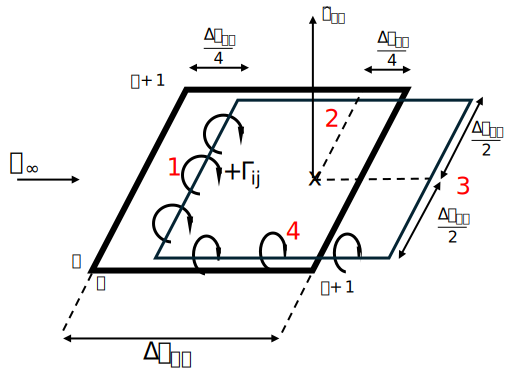
\includegraphics[width=0.8\textwidth]{Quadrilateral vortex ring element.png}
  \caption{Απεικόνιση στοιχείου \textlatin{Vortex Ring Element}}
  \label{fig:VortexRingElement}
\end{figure}



Οι αριθμοί 1 έως 4 στo \autoref{fig:VortexRingElement}, αντιπροσωπεύουν τα τέσσερα πεπερασμένα ευθύγραμμα τμήματα δινών που συνθέτουν το στοιχείο. Η επαγόμενη ταχύτητα του στοιχείου μπορεί να υπολογιστεί χρησιμοποιώντας την εξίσωση \eqref{eq:V12} σε κάθε τμήμα ξεχωριστά. Για ένα αυθαίρετο σημείο στον χώρο $P(x,y,z)$, η επαγόμενη ταχύτητα είναι:

\begin{equation}
{\vec{V}}_{P} = {\vec{V}}_{1} + {\vec{V}}_{2} + {\vec{V}}_{3} + {\vec{V}}_{4}
\end{equation}

Όπου:

\begin{equation}
    \label{eq:Vi}
{\vec{V}}_{i} = \frac{\Gamma}{4\pi}\ \frac{{\vec{r}}_{i,1} \times {\vec{r}}_{i,2}}{\left| {\vec{r}}_{i,1} \times {\vec{r}}_{i,2} \right|}({\vec{r}}_{i,1} - {\vec{r}}_{i,2}) \cdot \left( \frac{{\vec{r}}_{i,1}}{\left| {\vec{r}}_{i,1} \right|} - \frac{{\vec{r}}_{i,2}}{\left| {\vec{r}}_{i,2} \right|} \right)
\end{equation}

Όπως φάινεται στο \autoref{fig:Vortex ring elements in a grid}, αυτά τα στοιχεία ταξινομούνται σε ένα δισδιάστατο πλέγμα για να καλύψουν το σχήμα της ανυψωτικής επιφάνειας. Για να ικανοποιηθεί η συνθήκη \textlatin{Kutta}, η επίδραση της πίσω δίνης της τελευταίας σειράς πάνελ πρέπει να ακυρωθεί. Επομένως, η τελευταία σειρά πάνελ καθώς και όλα τα πάνελ του απόρρου πρέπει να έχουν την ίδια κυκλοφορία $\Gamma$.

\begin{figure}[H]
    \centering
    \includegraphics[width=\textwidth]{vortex ring model.png}
    \caption{\textlatin{Vortex ring elements} σε πλέγμα \cite{katz2001}}
    \label{fig:Vortex ring elements in a grid}
\end{figure}


Ο συντελεστής επιρροής \(\alpha_{ij}\) είναι ουσιαστικά η επαγόμενη ταχύτητα του \textlatin{i}-οστου στοιχείου δίνης με μοναδιαία κυκλοφορία στο \textlatin{j}-οστό σημείο ολοκλήρωσης. Οι συντελεστές επιρροής μπορούν να υπολογιστούν εύκολα χρησιμοποιώντας την εξίσωση \eqref{eq:Vi}. Επαναλαμβάνονας τον υπολογισμό για όλα τα πάνελ και όλα τα σημεία ολοκλήρωσης οδηγεί σε έναν πίνακα.

\begin{equation}
A = \begin{bmatrix}
a_{11} & a_{12} & \cdots & a_{1m} \\
a_{21} & a_{22} & \cdots & a_{2m} \\
 \vdots & \vdots & \ddots & \vdots \\
a_{m1} & a_{m2} & \cdots & a_{mm}
\end{bmatrix}
\end{equation}

\begin{figure}[H]
  \centering
  \includegraphics[width=\textwidth]{2D ARRAY OF PANELS.png}
  \caption{Διάταξη από \textlatin{wing} και \textlatin{wake panels} \cite{katz2001}}
\end{figure}

Για λόγους πληρότητας, το σύνολο των γραμμικών εξισώσεων που πρέπει να λυθεί προκειμένου να υπολογιστεί η ένταση της κυκλοφορίας κάθε στοιχείου για μια δεδομένη γωνία προσβολής για κάθε πάνελ είναι:

\begin{equation}
\begin{bmatrix}
a_{11} & a_{12} & \cdots & a_{1m} \\
a_{21} & a_{22} & \cdots & a_{2m} \\
 \vdots & \vdots & \ddots & \vdots \\
a_{m1} & a_{m2} & \cdots & a_{mm}
\end{bmatrix}\begin{bmatrix}
\Gamma_{1} \\
\Gamma_{2} \\
 \vdots \\
\Gamma_{m}
\end{bmatrix} = \begin{bmatrix}
 - {\vec{Q}}_{\infty} \cdot {\hat{n}}_{1} \\
 - {\vec{Q}}_{\infty} \cdot {\hat{n}}_{2} \\
 \vdots \\
 - {\vec{Q}}_{\infty} \cdot {\hat{n}}_{m}
\end{bmatrix}
\end{equation}


Η καθοδική ροή που προκαλείται σε κάθε στοιχείο δακτυλίου δίνης μπορεί να υπολογιστεί με ένα άλλο σύνολο γραμμικών εξισώσεων.

\begin{equation}
\begin{bmatrix}
{w_{ind}}_{1} \\
{w_{ind}}_{2} \\
 \vdots \\
{w_{ind}}_{m}
\end{bmatrix} = \begin{bmatrix}
b_{11} & b_{12} & \cdots & b_{1m} \\
b_{21} & b_{22} & \cdots & b_{2m} \\
 \vdots & \vdots & \ddots & \vdots \\
b_{m1} & b_{m2} & \cdots & b_{mm}
\end{bmatrix}\begin{bmatrix}
\Gamma_{1} \\
\Gamma_{2} \\
 \vdots \\
\Gamma_{m}
\end{bmatrix}
\end{equation}


Η άντωση και η αντίσταση μπορούν στη συνέχεια να υπολογιστούν χρησιμοποιώντας τις σχέσεις:

\begin{multline}
    L = \sum_{i = 1}^{M} \sum_{j = 1}^{N} \Delta L_{ij}, \\
    \text{Όπου} \quad \Delta L_{ij} = \begin{cases}
      \rho Q_{\infty} \left( \Gamma_{i,j} - \Gamma_{i - 1,j} \right) \Delta y_{ij}, & \text{γιά } i > 1 \\
      \rho Q_{\infty} \Gamma_{ij} \Delta y_{ij}, & \text{γιά } i = 1
    \end{cases}
  \end{multline}

\begin{multline}
D = \sum_{i = 1}^{M} \sum_{j = 1}^{N} \Delta D_{ij}, \\
\text{Όπου} \quad \Delta D_{ij} = \begin{cases}
    \rho w_{\text{ind}_{i,j}} \left( \Gamma_{i,j} - \Gamma_{i - 1,j} \right) \Delta y_{ij}, & \text{γιά } i > 1 \\
    \rho w_{\text{ind}_{i,j}} \Gamma_{ij} \Delta y_{ij}, & \text{γιά } i = 1
\end{cases}
\end{multline}


\section{Εξισώσεις Ανάλυσης Πτερυγισμού}\label{flutter-analysis-equations}

Η γενική μορφή της αεροελαστικής εξίσωσης κίνησης είναι \cite{AeroelasticityWright}

\begin{equation}
    \lbrack A\rbrack\ddot{q} + \left( \rho V\lbrack B\rbrack + D \right)\dot{q} + \left( \rho V^{2}\lbrack C\rbrack + \lbrack E\rbrack \right)q = \lbrack 0\rbrack  
\end{equation}



Όπου:

\begin{itemize}
  \item
    $[A]$, $[C]$, και $[E]$, είναι οι πίνακες που αντιστοιχούν στους $[M]$, $[C]$ και
    $[K]$ που είναι ο κλασικός συμβολισμός που χρησιμοποιείται στην ανάλυση ταλαντώσεων.
  \item
    $[B]$ και $[C]$ είναι οι αεροδυναμικοί πίνακες που εξαρτώνται από τον αριθμό \textlatin{Mach}
    και τη μειωμένη συχνότητα \textlatin{reduced frequency}. Ο τρόπος υπολογισμού αυτών των πινάκων μπορεί να
    ποικίλλει ανάλογα με την αεροδυναμική θεωρία που χρησιμοποιείται.
  \item
    $q$ είναι οι γενικευμένες συντεταγμένες.
  \end{itemize}
  
  


  \subsection{Σύνδεση της κατασκευής με την αεροδυναμική -- \textlatin{ Infinite Plate splines}}\label{interconnection-of-the-structure-with-aerodynamics-infinite-plate-splines}

  Οι  κατασκευαστικοί και οι αεροδυναμικοί βαθμοί ελευθερίας συνδέονται μέσω παρεμβολής. Αυτό επιτρέπει την ανεξάρτητη επιλογή των σημείων πλέγματος (κόμβων) των κατασκευαστικών και αεροδυναμικών πινάκων, αποσυνδέοντας έτσι τις δύο διακριτοποιήσεις της γεωμετρίας. Αυτή η μέθοδος παρεμβολής ονομάζεται \textlatin{splining}. To \textlatin{spline} άπειρης πλάκας που φαίνεται στο \autoref{fig:Surface Spline coordinate system} (\textlatin{Infinite Plate Spline}) και χρησιμοποιείται εδώ, βασίζεται στην παραμόρφωση μιας θεωρητικά άπειρης πλάκας που υπόκειται σε σημειακά φορτία σε συγκεκριμένα σημεία. Τα \textlatin{splines} χρησιμοποιούνται για δύο διαφορετικούς σκοπούς. Ως παρεμβολέας δυνάμεων για τον υπολογισμό της ισοδύναμης κατανομής δυνάμεων στην κατασκευή και ως παρεμβολέας μετατόπισης για τον υπολογισμό ενός συνόλου αεροδυναμικών μετατοπίσεων δεδομένου ενός συνόλου κατασκευαστικών μετατοπίσεων. Μαθηματικά αυτό σημαίνει ότι:
  
  

\begin{equation}
F_{s} = \left\lbrack G_{s \rightarrow a} \right\rbrack F_{a},\ \ U_{a} = {\lbrack G}_{a \rightarrow s}\rbrack U_{s}
\end{equation}


Όπου:

\begin{itemize}
  \item
    $F_{s}$ και $F_{a}$ είναι τα διανύσματα κατασκευαστικών και αεροδυναμικών δυνάμεων.
  \item
    $U_{a}$ και $U_{s}$ είναι τα αεροδυναμικά και κατασκευαστικά διανύσματα μετατόπισης.
  \item
    $G_{s \rightarrow a}$ και $G_{a \rightarrow s}$ είναι οι πίνακες \textlatin{spline} που συνδέουν το κατασκευαστικό με το αεροδυναμικό πρόβλημα και αντίστροφα. Έχει αποδειχθεί με την αρχή του εικονικού έργου ότι ο ένας πίνακας \textlatin{spline} είναι ο ανάστροφος του άλλου. Δηλαδή: 
    $\left\lbrack G_{s \rightarrow a} \right\rbrack = {{\lbrack G}_{a \rightarrow s}\rbrack}^{T}$ .
  \end{itemize}

\begin{figure}[H]
  \centering
  \includegraphics[width=0.9\textwidth]{surface spline.png}
  \caption{Σύστημα συντεταγμένων \textlatin{Surface Spline} \cite{msc2021}}
  \label{fig:Surface Spline coordinate system}
\end{figure}

Το \textlatin{Infinite plate spline} και όλα τα άλλα επιφανειακά \textlatin{splines} χρησιμοποιούνται για να βρουν μια επιφάνεια της μορφής $w(x,y)$ για όλα τα σημεία $(x,y)$ όταν το $w$ είναι
γνωστό σε ένα διακριτό σύνολο σημείων $w_{i} = w\left( x_{i},y_{i} \right)$.

Το \textlatin{Infinite plate spline} μιμείται τη συμπεριφορά μιας άπειρης πλάκας υπό σημειακή φόρτιση. Η παραμόρφωση μιας τέτοιας πλάκας λόγω ενός ενιαίου συγκεντρωμένου φορτίου στο σημείο $\left( x_{i} = 0,\ y_{i} = 0 \right)$ ονομάζεται θεμελιώδης λύση. Η κυβερνητική εξίσωση είναι:



\begin{equation}
D\nabla^{4}(w) = D\frac{1}{r}\frac{d}{dr}\left\{ r\frac{d}{dr}\left\lbrack \frac{1}{r}\frac{d}{dr}\left( r\frac{dw}{dr} \right) \right\rbrack \right\} = q
\label{eq:splineequation}
\end{equation}

Η γενική λύση της ομογενούς μορφής της εξίσωσης \ref{eq:splineequation} είναι:

\begin{equation}
   w = C_{1} + C_{1}r^{2} + C_{2}\ln(r) + C_{3}r^{2}\ln(r) 
\end{equation}

Θέτοντας $C_{2} = \ 0\ $ για να παραμείνει η λύση πεπερασμένη στο $r = 0$, τότε η ολοκλήρωση από το $r = 0$ στο $r = \epsilon\ (small\ number)$ οδηγεί στο $C_{3} = \frac{P}{8\pi D}$. Έτσι, η θεμελιώδης λύση για συγκεντρωμένο φορτίο είναι:

\begin{equation} w = A + Br^{2} + \frac{P}{16\pi D}r^{2}\ln\left( r^{2} \right) \end{equation}

Η θεμελιώδης λύση μπορεί να υπερτεθεί για την επίλυση όλου του προβλήματος της πλάκας:

\begin{equation} w(x,y) = \alpha_{0} + \alpha_{1}x + \alpha_{2}y + \sum_{i = 1}^{N}{K_{i}(x,y)P_{i}} \end{equation}

Όπου:

\begin{itemize}
\item
  $K_{i}(x,y) = \frac{1}{16\pi D}r_{i}^{2}\ln\left( r_{i}^{2} \right)$
\item
  $r_{i}^{2} = \left( x - x_{i} \right)^{2} + \left( y - y_{i} \right)^{2}$
\item
  $P_{i}$ \textlatin{concentrated load at} $\left( x_{i},y_{i} \right)$
\end{itemize}

Οι $N+3$ άγνωστοι καθορίζονται από τις $N+3$ εξισώσεις.

\begin{equation}
\sum_{}^{}{Pi} = 0
\end{equation}

\begin{equation}
  \sum_{}^{}{x_{i}P_{i}} = 0
\end{equation}

\begin{equation}
  \sum_{}^{}{y_{i}P_{i}} = 0
\end{equation}

\begin{equation}
  w_{j} = a_{0} + a_{1}x_{j} + a_{2}y_{2} + \sum_{i = 1}^{N}K_{ij}P_{i},\ \ (\ j = 1,\ldots,\ N)  
\end{equation}

Όπου $K_{ij} = K_{i}\left( x_{j},y_{j} \right)$ καί
$K_{ij} = K_{ji},\ \ K_{ij} = 0\ \text{όταν}\ i = j$

Αυτές οι $N+3$ εξισώσεις μπορούν να εκφραστούν σε μορφή πίνακα:

\begin{equation}
\begin{bmatrix}
  \begin{array}{c}
    0 \\
    0 \\
    0 \\
    \hline
    w_{1} \\
    w_{2} \\
     \vdots \\
    w_{N}        
  \end{array}
\end{bmatrix} = \begin{bmatrix}
\begin{array}{cccccc}
  0 & 0 & 0 & 1 & \cdots & 1 \\
0 & 0 & 0 & x_{1} & \cdots & x_{N} \\
0 & 0 & 0 & y_{1} & \cdots & y_{N} \\
\hline 
1 & x_{1} & y_{1} & 0 & \cdots & K_{1N} \\
1 & x_{2} & y_{2} & K_{21} & \cdots & K_{2N} \\
 \vdots & \vdots & \vdots & \vdots & \cdots & \vdots \\
1 & x_{N} & y_{N} & K_{N1} & \cdots & 0
\end{array}
\end{bmatrix}
\begin{bmatrix}
  \begin{array}{c}
    a_{0} \\
    a_{1} \\
    a_{2} \\
    \hline
    P_{1} \\
    P_{2} \\
     \vdots \\
    P_{N}
        
  \end{array}
\end{bmatrix} = \lbrack C\rbrack\lbrack P\rbrack
\end{equation}

Τώρα που τα $a_{i}$ και $P_{i}$ είναι γνωστά, η παρεμβολή μπορεί να εφαρμοστεί σε οποιοδήποτε μέγεθος για κάθε σημείο στο επίπεδο $(x,y)$ χρησιμοποιώντας την ακόλουθη εξίσωση:

\begin{equation}
\left\{ w \right\} = \begin{bmatrix}
1 & x_{1} & y_{1} & K_{1,1} & K_{1,2} & \cdots & K_{1,n} \\
1 & x_{2} & y_{2} & K_{2,1} & K_{2,2} & \cdots & K_{2.m} \\
 \vdots & \vdots & \vdots & \vdots & \vdots & \cdots & \vdots \\
1 & x_{n} & y_{n} & K_{n,1}\  & K_{n,2} & \cdots & K_{n,n}\ 
\end{bmatrix} \cdot \lbrack C\rbrack^{- 1}\begin{bmatrix}
0 \\
0 \\
0 \\
w_{1} \\
w_{2} \\
 \vdots \\
w_{N}
\end{bmatrix}
\end{equation}

\subsection{Η μέθοδος επίλυσης πτερυγισμού \textlatin{PK}}
\label{the-pk-method-of-flutter-solution}

Η θεμελιώδης εξίσωση για την ανάλυση πτερυγισμού χρησιμοποιώντας τη μέθοδο $PK$ είναι \cite{msc2021}:

\begin{equation}
\left\lbrack M_{hh}p^{2} + \left( B_{hh} - \frac{1}{4}\rho cV\frac{Q_{hh}^{I}}{k} \right)p + \left( K_{hh} - \frac{1}{2}\rho V^{2}Q_{hh}^{R} \right)\  \right\rbrack \cdot \left\{ u_{h} \right\} = \underline{0}
\end{equation}


Όπου:

\begin{itemize} 
  \item $M_{hh} =$ πίνακας μάζας ιδιομορφών, συνήθως διαγώνιος. 
  \item $B_{hh} =$ πίνακας απόσβεσης ιδιομορφών. 
  \item $K_{hh} =$ πίνακας δυσκαμψίας ιδιομορφών, συνήθως διαγώνιος, μπορεί να είναι και μιγαδικός αν χρησιμοποιηθεί πραγματική απόσβεση. 
  \item $Q_{hh}(M,k) =$ πίνακας αεροδυναμικής δύναμης που είναι συνάρτηση του αριθμού $Mach$ και της μειωμένης συχνότητας $k = \frac{\omega\overline{c}}{2V}$.
  \item $Q_{hh}{R}, Q_{hh}{I}$ είναι τα πραγματικά και φανταστικά μέρη του πίνακα αεροδυναμικής δύναμης $Q_{hh}$ ή πίνακες αεροδυναμικής δυσκαμψίας και αεροδυναμικής απόσβεσης αντίστοιχα. 
  \item $k = \frac{\omega\overline{c}}{2V}$ μειωμένη συχνότητα \textlatin{reduced frequency}. 
  \item $M =$ αριθμός $Mach$. 
  \item $V = \ $ ταχύτητα. 
  \item $\rho =$ πυκνότητα ρευστού. 
  \item $\left\{ u_{h} \right\} =$ \textlatin{modal participation vector.}
  \item $p = \omega(\gamma \pm i)$ ιδιοτιμή. 
\end{itemize}


Η εξίσωση επαναδιατυπώνεται στη μορφή \textlatin{state-space} με μείωση τάξης.
\begin{equation}
    \label{eq:PKss}
\lbrack A - pI\rbrack\left\{ {\overline{u}}_{h} \right\} = 0
\end{equation}

Όπου:

\begin{equation}
\lbrack A\rbrack = - \begin{bmatrix}
\mathbf{\lbrack 0\rbrack} & \mathbf{\lbrack I\rbrack} \\
 - M_{hh}^{- 1}\left( K_{hh} - \frac{1}{2}\rho V^{2}Q_{hh}^{R} \right) & - M_{hh}^{- 1}\left( B_{hh} - \frac{1}{4}\rho cV\frac{Q_{hh}^{I}}{k} \right)
\end{bmatrix}
\end{equation}

\begin{equation}
  {\overline{u}}_{h} = \begin{bmatrix}
    u_{h} \\
    {\dot{u}}_{h}
    \end{bmatrix}\  
\end{equation}


Ο βασικός αλγόριθμος για τη μέθοδο $PK$ περιλαμβάνει τα ακόλουθα βήματα:

\begin{enumerate} 
  \def\labelenumi{\arabic{enumi}.} 
  \item Γίνεται μια αρχική εκτίμηση της ιδιοσυχνότητας για την ιδιομορφή. 
  \item Υπολογίζεται η μειωμένη συχνότητα $k$ και η ταχύτητα $V$.
  \item Προσδιορίζονται (με παρεμβολή) οι πίνακες αεροδυναμικής δυσκαμψίας και απόσβεσης $Q_{hh}{R}, Q_{hh}{I}$. 
  \item Προσδιορίζονται οι ιδιοσυχνότητες για το σύστημα σε αυτήν την πτητική συνθήκη χρησιμοποιώντας την εξίσωση \eqref{eq:PKss}. 
  \item Επιλέγεται η ιδιοσυχνότητα που ήταν πιο κοντά στην αρχική εκτίμηση και επαναλαμβάνονται τα βήματα 1-5 μέχρι να συγκλίνει η λύση για τη συχνότητα.
  \item Αποθηκεύεται η τελική ιδιοσυχνότητα και η απόσβεση της ιδιομορφής. 
  \item Εξετάζεται η επόμενη ιδιομορφή ενδιαφέροντος χρησιμοποιώντας την ίδια διαδικασία μέχρι να έχουν διερευνηθεί όλες οι ιδιομορφές. 
\end{enumerate}


\section{Τεχνικές βελτιστοποίησης} \label{optimization-techniques}

\subsection{Μέθοδος γραμμικής αναζήτησης \textlatin{Brent -- Dekker}} \label{brents-dekker-line-search-method}

Αυτός ο αλγόριθμος στοχεύει στην εύρεση του ελαχίστου μιας συνάρτησης μιας μεταβλητής χωρίς τη χρήση των παραγώγων της. Αυτός ο αλγόριθμος χρησιμοποιείται συνήθως για την εύρεση του ελαχίστου μιας συνάρτησης $g\left( \mathbf{x} \right)$ πολλαπλών μεταβλητών \cite{brent1973}. Για το σκοπό αυτό συχνά απαιτείται η ελαχιστοποίηση της ακόλουθης συνάρτησης

\begin{equation}
    \label{eq:minfun}
\gamma(\lambda) = f(\mathbf{x}_{0} + \lambda\mathbf{s})
\end{equation}

Όπου $\mathbf{x}_0$ και $\mathbf{s}$ είναι σταθερά και το $\lambda$ είναι μια βαυμωτή μεταβλητή. Το πρόβλημα αυτό περιγράφει ουσιαστικά μια μονοδιάστατη αναζήτηση ξεκινώντας από το $\mathbf{x}_0$ προς την κατεύθυνση του $\mathbf{s}$.

Ο αλγόριθμος βρίσκει μια προσέγγιση στο ελάχιστο μιας συνάρτησης $f$ ορισμένης στο διάστημα $\lbrack a,\ b\rbrack$. Υπάρχουν έξι σημαντικά σημεία $a,b,u,v,w$ και $x$ τα οποία δεν είναι όλα διακριτά. Μία πιθανή διάταξη των σημείων αυτών φαίνεται στο \autoref{fig:A possible configuration of points}. Αυτά τα σημεία αρχικοποιούνται ως εξής:

\begin{equation}
    \label{eq:brentspoints}
v = w = x = a + \left( \frac{3 - \sqrt{5}}{2} \right)(b - a)
\end{equation}

Ο αριθμός $\left( \frac{3 - \sqrt{5}}{2} \right)$ προέρχεται από τον αλγόριθμο αναζήτησης χρυσής τομής και είναι αυθαίρετη επιλογή. Τα σημεία που ορίζονται στην εξίσωση \eqref{eq:brentspoints} εξυπηρετούν ένα συγκεκριμένο σκοπό:

\begin{itemize} 
  \item Τα σημεία $a$ και $b$ ορίζουν το διάστημα μέσα στο οποίο βρίσκεται ένα τοπικό ελάχιστο. 
  \item $x$: από όλα τα σημεία στα οποία έχει υπολογιστεί η $f$, το $x$ είναι το σημείο με την ελάχιστη τιμή της $f$. 
  \item $w$ είναι το σημείο με την επόμενη χαμηλότερη τιμή του $f$. 
  \item $v$ είναι η προηγούμενη τιμή του $w$. 
  \item $u$ είναι το τελευταίο σημείο στο οποίο έχει υπολογιστεί η $f$.
\end{itemize}

\begin{figure}
  \centering
  \includegraphics[width=\textwidth]{brents_six_points.png}
  \caption{Μια πιθανή διαμόρφωση σημείων  \cite{brent1973} }
  \label{fig:A possible configuration of points}
\end{figure}

Μια τυπική επανάληψη του αλγόριθμου εξελίσσεται ως εξής:


\begin{enumerate} 
  \def\labelenumi{\arabic{enumi}.} 
  \item Έστω $m = 1\text{/}2(a + b)$ το μέσο του διαστήματος.

  \begin{enumerate} \def\labelenumii{\alph{enumii}.} 
      \item Αν $|x - m| \leq 2 \cdot tol - \frac{1}{2}(b - a)\ $, τότε ο αλγόριθμος τερματίζεται με το $x$ ως ελάχιστο. 
      \item Διαφορετικά, οι αριθμοί $p$ και $q$ υπολογίζονται έτσι ώστε $x + p/q$ να είναι το ελάχιστο της παραβολής που διέρχεται από τα σημεία\\ $\left( v,f(v) \right),\ \ \left( w,f(w) \right),\ \ \left( x,f(x) \right)$. 
  \end{enumerate} 

  \item Έστω $e$ η τιμή του $p/q$.
  
  \begin{enumerate} \def\labelenumii{\alph{enumii}.} 
    \item Αν $|e| \leq tol$,\ $q = 0$,\ $x + p\text{/}q \notin \lbrack a,b\rbrack$ ή $\left| p\text{/}q \right| \geq 1/2|e|$, τότε πραγματοποιείται το βήμα της χρυσής τομής:
  
    \begin{equation} u = \begin{cases} \frac{\sqrt{5} - 1}{2}x + \frac{3 - \sqrt{5}}{2}a, & \text{αν } x \geq m \\ \frac{\sqrt{5} - 1}{2}x + \frac{3 - \sqrt{5}}{2}b, & \text{αν } x < m \end{cases} \end{equation}
  
    \item Διαφορετικά $u = x + p\text{/}q$ (οι αποστάσεις $|u - x|,\ \ u - a,\ \ b - u\ $ πρέπει να είναι τουλάχιστον $tol$). 
  \end{enumerate}
\end{enumerate}


\begin{enumerate}
  \def\labelenumi{\arabic{enumi}.}
  \setcounter{enumi}{2}
  \item
    Η $f$ υπολογίζεται στο νέο σημείο $u$ και τα σημεία
    $a,b,v,w\ \text{και}\ x$ ενημερώνονται και ο κύκλος επαναλαμβάνεται.
  \end{enumerate}

  Ο αλγόριθμος συνήθως τερματίζει όταν $x = b - tol$ ή
  $x = a + tol$ μετά από την πραγματοποίηση μιας παραβολικής παρεμβολής, όπου
  έχει εφαρμοστεί η συνθήκη ότι $|u - x| \geq tol$. Το επόμενο
  σημείο παραβολικής παρεμβολής βρίσκεται κοντά στα $x$ και $b$, επομένως το $u$ είναι αναγκαστικά
  $x - tol$. Μια τυπική κατάσταση στην οποία ο αλγόριθμος τερματίζει φαίνεται στο \autoref{fig:typical terminal configuration of important points}

\begin{figure}[H]
    \centering
    \includegraphics[width=\textwidth]{brents algorithm termination configuration.png}
    \caption{Τυπική τερματική διαμόρφωση σημαντικών σημείων \cite{brent1973}}
    \label{fig:typical terminal configuration of important points}

\end{figure}

\subsection{Η Μέθοδος του \textlatin{Powell}}
\label{powells-method}

Η μέθοδος του \textlatin{Powell} είναι μια τροποποιημένη κυκλική αναζήτηση συντεταγμένων. Και οι δύο μέθοδοι στοχεύουν στην ελαχιστοποίηση μιας συνάρτησης πολλών μεταβλητών χωρίς να χρησιμοποιούν καμία από τις παραγώγους της. Γι' αυτό αποκαλούνται μέθοδοι μηδενικής τάξης.

Η μέθοδος κυκλικής αναζήτησης συντεταγμένων είναι στην ουσία μια σειρά βελτιστοποιήσεων γραμμικής αναζήτησης που εκτελούνται κυκλικά σε όλες τις παραμέτρους της συνάρτησης. Η αναζήτηση ξεκινά από ένα αρχικό $x^{(0)}$ και βελτιστοποιεί την πρώτη παράμετρο:

\begin{equation}
\mathbf{x}^{(1)} = \arg_{x_{1}}{\min{f\left( x_{1},x_{2}^{(0)},\ldots,x_{n}^{(0)} \right)}}
\end{equation}

Αφού βρεθεί αυτό, βελτιστοποιεί την επόμενη παράμετρο:

\begin{equation}
\mathbf{x}^{(2)} = \arg_{x_{2}}{\min{f\left( x_{1}^{(1)},x_{2},\ldots,x_{n}^{(1)} \right)}}
\end{equation}

Αυτό μπορεί επίσης να εκφραστεί με τη βοήθεια της εξίσωσης \eqref{eq:minfun} αν $\mathbf{s}$ είναι το \textlatin{i}-οστό διανύσμα βάσης για $i = 1,\ldots,n$.

Μπορεί να χρησιμοποιηθεί οποιοσδήποτε αλγόριθμος γραμμικής αναζήτησης, αλλά ο αλγόριθμος του \textlatin{Brent} βρίσκει ευρεία χρήση σε βιβλιοθήκες βελτιστοποίησης, συμπεριλαμβανομένης της υλοποίησης της μεθόδου \textlatin{Powell} στήν  \textlatin{SciPy}.

\begin{figure}[H]
    \centering
    \includegraphics[width=0.5\textwidth]{cyclic coordinate search.png}
    \caption{Η μέθοδος \textlatin{Cyclic Coordinate Search \cite{kochenderfer2019}}}
    \label{fig:CCsearch}
\end{figure}

Όπως φαίνεται στo \autoref{fig:CCsearch}, ένα μειονέκτημα αυτής της μεθόδου είναι η αργή
προσπέλαση των διαγώνιων κοιλάδων, όπου γίνονται επαναλαμβανόμενα μικρά βήματα σε
κάθε κατεύθυνση. Η ιδέα του \textlatin{M.J.D. Powell} ήταν να επεκτείνει την κυκλική
αναζήτηση συντεταγμένων ώστε να μπορεί να αναζητά σε κατευθύνσεις που
δεν είναι κάθετες μεταξύ τους και ούτε τα διανύσματα βάσης. Για να
επιτευχθεί αυτή η νέα ικανότητα, ο αλγόριθμος του \textlatin{Powell} διατηρεί μια λίστα
κατευθύνσεων αναζήτησης
$\left\lbrack \mathbf{u}^{(0)},\ldots\mathbf{u}^{(n)} \right\rbrack$
οι οποίες αρχικά είναι τα διανύσματα βάσης συντεταγμένων
$\mathbf{u}^{(i)}=\mathbf{e}^{\left( \mathbf{i} \right)}$ για
όλα τα $i$.

Ξεκινώντας από το $\mathbf{x}^{(0)}$, η μέθοδος του \textlatin{Powell} διεξάγει μια γραμμική αναζήτηση όπως και πριν, για κάθε κατεύθυνση αναζήτησης διαδοχικά:


\begin{equation}
\mathbf{x}^{(i + 1)} \leftarrow linesearch\left( f,\mathbf{x}^{(i)}\mathbf{,}\mathbf{u}^{(i)} \right)\mathbf{\ }for\ i\ in\ \lbrack 0,\ldots,n\rbrack
\end{equation}

Στη συνέχεια, όλες οι κατευθύνσεις αναζήτησης μετατοπίζονται κατά έναν δείκτη,
απορρίπτοντας την παλαιότερη κατεύθυνση αναζήτησης, $\mathbf{u}^{(0)}\ $

\begin{equation}
\mathbf{u}^{(i)} \leftarrow \mathbf{u}^{(i + 1)}\ for\ i\ in\ \lbrack 0,\ldots,n - 1\rbrack
\end{equation}

Η τελευταία κατεύθυνση αναζήτησης αντικαθίσταται με την κατεύθυνση από
το $\mathbf{x}^{(0)}$ στο $\mathbf{x}^{(n + 1)}$, που είναι η συνολική
κατεύθυνση της προόδου κατά τις τελευταίες $n$ γραμμικές αναζητήσεις:

\begin{equation}
\mathbf{u}^{(n)} \leftarrow \mathbf{x}^{(n + 1)} - \mathbf{x}^{(0)}
\end{equation}

Αυτή η διαδικασία επαναλαμβάνεται μέχρι τη σύγκλιση.
\begin{figure}[H]
    \centering
    \includegraphics[width=0.5\textwidth]{powells method.png}
    \caption{Η μέθοδος \textlatin{Powell} \cite{kochenderfer2019}}
    \label{fig:Powell}

\end{figure}

Όπως φαίνεται στο \autoref{fig:Powell}, η μέθοδος του Powell ξεκινά όπως η κυκλική
αναζήτηση συντεταγμένων αλλά σταδιακά ((μαθαίνει)) την κατεύθυνση μέγιστης καθόδου.


\subsection{Γενετικός Αλγόριθμος}
\label{genetic-algorithm}

Οι γενετικοί αλγόριθμοι μιμούνται τη λογική της Δαρβινικής εξέλιξης, όπου τα
καταλληλότερα ((άτομα)) είναι πιο πιθανό να μεταβιβάσουν τα γονίδιά τους στην επόμενη
γενιά. Τα χρωμοσώματα κάθε ατόμου ορίζουν ένα μόνο σημείο σχεδίασης. Σε κάθε γενιά, τα χρωμοσώματα των καταλληλότερων ατόμων μεταβιβάζονται στην επόμενη γενιά αφού περάσουν απο τα στάδια της \emph{διασταύρωσης, (\latintext{crossover})}  και της \emph{μετάλλαξης, \latintext(mutation)}.

Τα χρωμοσώματα συχνά αναπαρίστανται από ένα λογικό πίνακα, αλλά σε αυτήν την περίπτωση ένας πίνακας πραγματικών τιμών περιγράφει καλύτερα το χώρο σχεδίασης.

\subsubsection{Αρχικοποίηση}

Ο Γενετικός Αλγόριθμος ξεκινά με την αρχικοποίηση ενός πληθυσμού με τυχαία χρωμοσώματα.

\subsubsection{Επιλογή Γονέων}

Η διαδικασία επιλογής είναι η διαδικασία επιλογής των χρωμοσωμάτων που θα δημιουργήσουν απογόνους για την επόμενη γενιά μετά από την υποβολή στις γενετικές διαδικασίες της διασταύρωσης και της μετάλλαξης. Υπάρχουν πολλές μέθοδοι επιλογής των ατόμων που θα ζευγαρώσουν και θα συνδυάσουν τα γονίδιά τους. Μερικές από τις πιο δημοφιλείς περιλαμβάνουν:

\begin{itemize}
\item
  \textlatin{Roulette Wheel selection:} Όπου στο κάθε άτομο έχει ανατεθεί μέρος της
  φανταστικής ρουλέτας ανάλογη με την απόδοσή τους. Στη συνέχεια, η ρουλέτα
  περιστρέφεται μέχρι να επιτευχθεί ο επιθυμητός αριθμός γονέων. Αυτή η μέθοδος είναι
  απλή και αποτελεσματική στις περισσότερες περιπτώσεις. Μπορεί να επηρεαστεί ωστόσο από
  άτομα που είναι πολύ αποδοτικότερα από τον υπόλοιπο πληθυσμό.
\item
  \textlatin{Tournament Selection}: Ένα υποσύνολο ατόμων επιλέγεται τυχαία
  και το καλύτερο άτομο από αυτά επιλέγεται ως γονέας. Η
  διαδικασία επαναλαμβάνεται μέχρι να επιτευχθεί ο επιθυμητός αριθμός γονέων.
\item
\textlatin{Steady State Crossover}: Ένα σταθερό μέρος του πληθυσμού αντικαθίσταται
  σε κάθε γενιά. Μόνο τα αδύναμα άτομα αντικαθίστανται από
  απογόνους, αυτή η μέθοδος διασφαλίζει ότι το καταλληλότερο άτομο
  διατηρείται τις περισσότερες φορές. Ένα μειονέκτημα αυτής της μεθόδου είναι ότι αργεί να προσαρμοστεί, καθώς μόνο ένα μικρό μέρος του πληθυσμού αντικαθίσταται σε κάθε γενιά.
\end{itemize}

\subsubsection{\textlatin{Crossover}}

Η διασταύρωση (\textlatin{Crossover}) είναι ο τρόπος με τον οποίο τα χρωμοσώματα των γονέων συνδυάζονται για
τη δημιουργία απογόνων. Υπάρχουν διάφοροι τρόποι διασταύρωσης. Οι πιο
κοινώς χρησιμοποιούμενοι είναι:
\begin{samepage}
\begin{itemize}
\item
\textlatin{Single point crossover}

Με αυτόν τον τρόπο, το πρώτο τμήμα του χρωμοσώματος του γονέα A σχηματίζει το πρώτο τμήμα του χρωμοσώματος του παιδιού και το τελευταίο τμήμα του χρωμοσώματος του γονέα B σχηματίζει το τελευταίο τμήμα του χρωμοσώματος του παιδιού. Η διαδικασία αυτή φάινεται στο \autoref{fig:Single Point Crossover}


\begin{figure}[H]
    \centering
    \includegraphics[width=\textwidth]{single point crossover.png}
    \caption{Διασταύρωση \textlatin{(Crossover)} ενός σημείου \cite{kochenderfer2019}}
    \label{fig:Single Point Crossover}


\end{figure}


\item
\textlatin{Two point crossover}

Όπως πριν, αλλά όπως φαίνεται στο \autoref{fig:Two-point Crossover} προστίθεται ένα δεύτερο σημείο διασταύρωσης.


\begin{figure}[H]
    \centering
    \includegraphics[width=\textwidth]{two point crossover.png}
    \caption{Διασταύρωση \textlatin{(Crossover)} δύο σημείων \cite{kochenderfer2019}}
    \label{fig:Two-point Crossover}


\end{figure}

\item
\textlatin{Uniform crossover}

Κατά αυτόν τον τρόπο, όπως φάινεται στο \autoref{fig:Uniform Crossover} κάθε χρωμόσωμα έχει 50\% πιθανότητα να προέρχεται από τον γονέα A ή τον γονέα B.

\begin{figure}[H]
    \centering
    \includegraphics[width=\textwidth]{uniform crossover.png}
    \caption{Ομοιόμορφη διασταύρωση \textlatin{(Uniform Crossover) \cite{kochenderfer2019}}}
    \label{fig:Uniform Crossover}

\end{figure}
\end{itemize}
\end{samepage}

\subsubsection{\textlatin{Mutation}}

Η μετάλλαξη είναι ένα απαραίτητο βήμα του γενετικού αλγορίθμου, καθώς επιτρέπει την ανάπτυξη νέων χαρακτηριστικών που δεν υπήρχαν στον αρχικό πληθυσμό. Στην ουσία, μια τυχαία τιμή προστίθεται σε ένα τυχαίο χρωμόσωμα ενός τυχαία επιλεγμένου απογόνου. Η πιθανότητα να συμβεί μια μετάλλαξη σε ένα άτομο ονομάζεται \textlatin{\emph{mutation rate}}.

\subsubsection{\textlatin{Elitism}}

Ο ελιτισμός είναι μια στρατηγική που διασφαλίζει ότι ένας σταθερός αριθμός των καταλληλότερων
ατόμων επιβιώνει στην επόμενη γενιά.

Οι γενετικοί αλγόριθμοι έχουν ένα πολύ ευρύ φάσμα εφαρμογών και είναι πολύ προσαρμόσιμοι σε πολλά προβλήματα. Όμως υπάρχει ένα πρόβλημα. Όλες αυτές οι παράμετροι και στρατηγικές επηρεάζουν σημαντικά τα αποτελέσματα και δεν υπάρχει καμία τυπική μέθοδος επιλογής κάθε παραμέτρου. Επομένως, είναι ευθύνη του ερευνητή να κατανοήσει το πρόβλημα και μέσω πειραματισμού και τεχνικών ρύθμισης υπερπαραμέτρων μοντέλου, να καθορίσει ένα
αρκετά καλό σύνολο παραμέτρων.

\subsection{Νευρωνικά Δίκτυα}
\label{neural-networks}

\subsubsection{Τι είναι τα Τεχνητά Νευρωνικά Δίκτυα \textlatin{(ANN's)}}

Ένα τεχνητό νευρωνικό δίκτυο είναι ένα υπολογιστικό μοντέλο που εμπνέεται από τον τρόπο λειτουργίας του βιολογικού εγκεφάλου. Η βασική δομή ενός \textlatin{ANN} αποτελείται από διασυνδεδεμένους κόμβους (ή νευρώνες) οργανωμένους σε στρώματα.

Η βασική μονάδα αυτής της δομής είναι ο νευρώνας, μια απεικόνιση του οποίου φαίνεται	στο \autoref{fig:The Structure of a Neuron} . Ένας νευρώνας έχει πολύ απλή δομή. Δέχεται έναν αυθαίρετο αριθμό εισόδων μαζί με μια σταθερά προσαύξησης (\textlatin{bias}) και έχει μόνο μία έξοδο. Η έξοδος μπορεί να είναι λογική ή πραγματική. Εντός του νευρώνα, πραγματοποιείται ένα άθροισμα χρησιμοποιώντας το βάρος κάθε εισόδου και την σταθερά προσαύξησης. Το αποτέλεσμα κάθε αθροίσματος επεξεργάζεται περαιτέρω μέσω μιας ((συνάρτησης ενεργοποίησης)) (\textlatin{activation function}) και προκύπτει η έξοδος. Η συνάρτηση ενεργοποίησης επιτρέπει τη μη γραμμική συμπεριφορά των νευρωνικών δικτύων. Μπορεί να είναι οποιαδήποτε συνάρτηση, αλλά ορισμένες συναρτήσεις έχουν επικρατήσει.

\begin{figure}[H]
    \centering
    \includesvg[width=\textwidth]{Neuron.svg}
    \caption{Η δομή ενός νευρώνα}
    \label{fig:The Structure of a Neuron}
    

\end{figure}


Η βασική αρχιτεκτονική ενός νευρωνικού δικτύου φαίνεται στο \autoref{fig:Structure of a Neural Network} και  αποτελείται από:

\begin{enumerate}
\def\labelenumi{\arabic{enumi}.}
\item
  Ένα στρώμα εισόδου το οποίο είναι υπεύθυνο για τη λήψη των αρχικών δεδομένων. 
  Κάθε νευρώνας στο στρώμα εισόδου αντιπροσωπεύει ένα συγκεκριμένο χαρακτηριστικό των δεδομένων εισόδων.
\item
  Κρυφά στρώματα, τα οποία είναι ενδιάμεσα στρώματα μεταξύ των στρωμάτων εισόδου και
  εξόδου και είναι υπεύθυνα για την αναγνώριση σύνθετων χαρακτηριστικών.
\item
  Τα βάρη και οι σταθερές προσαύξησης που χρησιμοποιούνται στο νευρωνικό δίκτυο, και τα οποία είναι οι παράμετροι που πρέπει να εκπαιδευτούν για να μπορέσει το νευρωνικό δίκτυο
  να κάνει ουσιαστικές προβλέψεις.
\item
  Ένα στρώμα εξόδου το οποίο παράγει τις τελικές προβλέψεις. Η έξοδος μπορεί
  να είναι δυαδική για προβλήματα ταξινόμησης ή κλιμακωτή για προβλήματα παλινδρόμησης.
\end{enumerate}

\begin{figure}[H]
    \centering
    \includesvg[width=\textwidth]{Neural Network.svg}
    \caption{Η δομή ενός νευρωνικού δικτύου \cite{takyar2025}}
    \label{fig:Structure of a Neural Network}


\end{figure}

Ο αριθμός των κρυφών στρωμάτων σε ένα νευρωνικό δίκτυο μπορεί να διαφέρει. Τα νευρωνικά δίκτυα που δεν έχουν κρυφά στρώματα ονομάζονται Ρηχά (\textlatin{shallow}), ενώ τα νευρωνικά δίκτυα με κρυφά στρώματα ονομάζονται Βαθιά Νευρωνικά Δίκτυα \textlatin{(Deep Neural Networks)}.


\subsubsection{Εκπαίδευση Τεχνητών Νευρωνικών Δικτύων}

Όπως αναφέρθηκε προηγουμένως, για να είναι χρήσιμο ένα νευρωνικό δίκτυο πρέπει να εκπαιδευτεί. Η εκπαίδευση περιλαμβάνει τη συλλογή δεδομένων παρόμοιων με αυτά που το \textlatin{ΝΝ} προορίζεται να προβλέψει, και την εκτέλεση μιας βελτιστοποίησης των βαρών και των προσαυξήσεων εντός του δικτύου για την ελαχιστοποίηση κάποιας συνάρτησης απώλειας \textlatin{loss function}. Μια συνάρτηση απώλειας είναι ένα μέτρο του ποσού του σφάλματος πρόβλεψης. Υπάρχουν πολλές συναρτήσεις απώλειας που χρησιμοποιούνται συνήθως για τα νευρωνικά δίκτυα, αλλά όταν ένα νευρωνικό δίκτυο εκπαιδεύεται σε ένα πρόβλημα παλινδρόμησης, η συνάρτηση απώλειας είναι συνήθως μία από τις ακόλουθες:

\foreignlanguage{english}{
\begin{enumerate}
\def\labelenumi{\arabic{enumi}.}
\item
  Mean Squared Error (MSE)
\end{enumerate}

\begin{equation}
MSE = \frac{1}{N}\sum_{i = 1}^{N}\left( y_{i} - \hat{y} \right)^{2}
\end{equation}


\begin{enumerate}
\def\labelenumi{\arabic{enumi}.}
\setcounter{enumi}{1}
\item
  Root Mean Squared Error
\end{enumerate}

\begin{equation}
RMSE = \ \sqrt{MSE} = \sqrt{\frac{1}{N}\sum_{i = 1}^{N}\left( y_{i} - \hat{y} \right)^{2}}
\end{equation}

\begin{enumerate}
\def\labelenumi{\arabic{enumi}.}
\setcounter{enumi}{2}
\item
  Mean Average Error (MAE)
  
  \begin{equation}
    MAE = \frac{1}{N}\sum_{i = 1}^{N}{|y_{i} - \hat{y}|}
    \label{eq:MAE}
  \end{equation}
  \textgreek{Όπου: $\hat{y}$ είναι η προβλεπόμενη τιμή του $y$}
\end{enumerate}
}

O στόχος της εκπαίδευσης του νευρωνικού δικτύου είναι η ελαχιστοποίηση οποιασδήποτε από αυτές τις συναρτήσεις στα δεδομένα δοκιμής που το δίκτυο δεν έχει ξαναδεί.

Για να επιτευχθεί αυτός ο στόχος, πρώτα τα διαθέσιμα δεδομένα που περιέχουν τόσο την είσοδο όσο και την επιθυμητή έξοδο, χωρίζονται τυχαία σε δεδομένα εκπαίδευσης (\textlatin{training data}) (αυτά που θα χρησιμοποιηθούν για την προσαρμογή των βαρών και των προσαυξήσεων) και δεδομένα δοκιμής (\textlatin{test data}) (αυτά που θα χρησιμοποιηθούν για την αξιολόγηση της απόδοσης του νευρωνικού δικτύου). Στη συνέχεια, μέσω μιας διαδικασίας που ονομάζεται \textlatin{backpropagation} (η ακριβής εξήγηση της οποίας είναι πέρα από το πεδίο αυτής της διατριβής) σε παρτίδες των δεδομένων εκπαίδευσης, τα βάρη ενημερώνονται με τέτοιο τρόπο ώστε να μειωθεί η τιμή της συνάρτησης απώλειας για αυτό το συγκεκριμένο σύνολο δεδομένων. Μόλις όλες οι παρτίδες δεδομένων έχουν περάσει από το δίκτυο και τα βάρη έχουν προσαρμοστεί ανάλογα, λέμε ότι το δίκτυο έχει ολοκληρώσει ένα πέρασμα μέσω των δεδομένων εκπαίδευσης. Αυτή η διαδικασία εκτιμά την κλίση της συνάρτησης απώλειας και έτσι το δίκτυο κατεβαίνει προς το ελάχιστο της συνάρτησης απώλειας. Ο αριθμός των επαναλήψεων αυτής της διαδικασίας ονομάζεται \textlatin{epochs}. Ο αριθμός των \textlatin{epochs} πρέπει να είναι τέτοιος ώστε να επιτευχθεί μια βέλτιστη λύση χωρίς την υπερπροσαρμογή \textlatin{(overfitting)} του δικτύου στα δεδομένα εκπαίδευσης.

\subsubsection{\textlatin{Hyperparameter Tuning}}

Όπως έχουμε δει, για να ορίσουμε ένα νευρωνικό δίκτυο, πρέπει να επιλέξουμε πολλές παραμέτρους εκ των προτέρων. Αυτές οι παράμετροι περιλαμβάνουν τον αριθμό των κρυφών στρωμάτων, τον αριθμό των νευρώνων σε κάθε στρώμα, και τη συνάρτηση ενεργοποίησης κάθε στρώματος,καθώς και πολλές άλλες. Το βέλτιστο σύνολο παραμέτρων δεν είναι γνωστό εκ των προτέρων και δεν υπάρχει μέθοδος επιλογής του.

Η διαδικασία βελτιστοποίησης των υπερπαραμέτρων ενός μοντέλου ονομάζεται \emph{\textlatin{Hyperparameter Tuning}}. Υπάρχουν πολλοί αλγόριθμοι βελτιστοποίησης που το επιτυγχάνουν αυτό. Ένας από τους πιο ενδιαφέροντες και αυτός που θα χρησιμοποιηθεί για αυτή την εφαρμογή είναι ο αλγόριθμος \textlatin{HyperBand} \cite{li2018hyperbandnovelbanditbasedapproach}. Ο αλγόριθμος αυτός είναι μια βελτίωση του αλγόριθμου \textlatin{Successive Halving}.

Η ιδέα πίσω από τον αλγόριθμο \textlatin{Successive Halving} είναι αρκετά απλή. Κατανέμει ομοιόμορφα έναν προϋπολογισμό πόρων (υπολογιστικού χρόνου) σε ένα σύνολο υπερπαραμέτρων, αξιολογεί την απόδοση κάθε σετ υπερπαραμέτρων, απορρίπτει το χειρότερο 50\% και επαναλαμβάνει μέχρι να απομείνει ένα μόνο σετ υπερπαραμέτρων. Το πρόβλημα με αυτόν τον αλγόριθμο είναι ότι δεν είναι γνωστό εάν η δοκιμή ενός μεγαλύτερου αριθμού διαμορφώσεων με περιορισμένους υπολογιστικούς πόρους η καθεμία ή ενός μικρότερου αριθμού διαμορφώσεων με περισσότερους πόρους, θα έχει καλύτερο αποτέλεσμα.

Αυτό είναι το πρόβλημα που αντιμετωπίζει ο αλγόριθμος \textlatin{HyperBand}. Η αντιμετώπιση επιτυγχάνεται πραγματοποιώντας ένα \textlatin{grid search} για τις εφικτές τιμές των $n$ και $r$, όπου $n$ είναι ο αριθμός των διαμορφώσεων που θα δοκιμαστούν και $r$ είναι η ελαχιστη ποσότητα υπολογιστικής ισχύος που κατανέμεται σε όλες τις διαμορφώσεις πρωτού δύναται να απορριφθούν.


    \chapter{Μεθοδολογία}
\label{Ch:methodology}
\chapterprecis{
Σε αυτό το κεφάλαιο, το θεωρητικό υπόβαθρο που αναπτύχθηκε στο \autoref{Ch:Theory} θα εφαρμοστεί για την επίλυση ενός πραγματικού προβλήματος. Το κεφάλαιο αυτό εξηγήσει το πρόβλημα που πρέπει να επιλυθεί, τον τρόπο με τον οποίο   δημιουργείται το μοντέλο αεροελαστικής ανάλυσης καθώς και τη διαδικασία που χρησιμοποιείται για τη βελτιστοποίηση του.}

\section{Εισαγωγή στο Πρόβλημα}
\label{problem-introduction}

Το πρόβλημα που έχει επιλεγεί ως παράδειγμα εφαρμογής της θεωρίας που αναπτύχθηκε στο προηγούμενο κεφάλαιο είναι η μελέτη των χαρακτηριστικών πτερυγισμού της κύριας πτέρυγας του ανεμοπλάνου \textlatin{ASW 28} και η  βελτιστοποίηση του σχεδιασμού, του σύνθετου υλικού του για να προσαρμοστούν τα χαρακτηριστικά του πτερυγισμού σε συγκεκριμένες απαιτήσεις. Η επιλογή αυτού του συγκεκριμένου αεροσκάφους έγινε λόγω του μεγάλου εκπετάσματος σε σχέση με το μήκος της χορδής του \textlatin{aspect ratio}, γεγονός που το καθιστά πολύ ευλύγιστο. Επιπλέον, ο κύριος στόχος ενός ανεμοπλάνου είναι να επιτύχει τo βέλτιστo λόγο καθόδου \textlatin{glide ratio}, επομένως η μείωση του βάρους είναι υψίστης σημασίας για αυτά τα οχήματα κάτι που τα καθιστά ιδανικά για αυτήν την εφαρμογή καθώς συνδυάζουν τη μεγάλη πιθανότητα εμφάνισης πτερυγισμού με την ανάγκη για ελαχιστοποίηση βάρους.

\textlatin{``The ASW 28 is Schleicher's high-performance glider for the
FAI-Standard Class with 15m span.'' \cite{asw28}}. Τα τεχνικά χαρακτηριστικά αυτού του αεροσκάφους συνοψίζονται στο \autoref{fig:TechnicalDataofASW28glider} :


\begin{figure}[H]
\centering
\includegraphics[width=2.92073in]{ASW28_characteristics.png}
\caption{Τεχνικά δεδομένα του ανεμοπλάνου \textlatin{ASW 28 \cite{asw28}}}
\label{fig:TechnicalDataofASW28glider}
\end{figure}

\begin{figure}[H]
\centering
\includegraphics[width=5.5026in,height=3.34935in]{ASW 28 3side view.png}
\caption{Εμπρόσθια, πλάγια και άνω όψη του ανεμοπλάνου  \textlatin{ASW 28 \cite{asw28}}}
\end{figure}

Η ανάλυση της κύριας πτέρυγας του \textlatin{ASW 28} θα περιλαμβάνει τα εξής βήματα:

\begin{enumerate}
  \def\labelenumi{\arabic{enumi}.}
  \item
    Δημιουργία μοντέλου στο \textlatin{HyperMesh} της \textlatin{Altair} για ανάλυση ιδιομορφών και πτερυγισμού.
  \item
    Δημιουργία κώδικα σε \textlatin{Python} για το αυτόματο διάβασμα των αποτελεσμάτων πτερυγισμού από τον επιλυτή \textlatin{Optistruct}.
  \item
    Ορισμός του προβλήματος βελτιστοποίησης χρησιμοποιώντας διάφορες τεχνικές βελτιστοποίησης και υλοποίηση αυτών με \textlatin{Python}.
  \end{enumerate}
  
  

  \section{Μοντέλο Κύριας Πτέρυγας \textlatin{ASW 28}}
  \label{asw-28-main-composite-wing-model}
  
  \subsection{Γεωμετρία Πτέρυγας \&\ Διακριτοποίηση Γεωμετρίας}\label{wing-geometry-discretization}
  
  Η εξωτερική γεωμετρία της πτέρυγας εισήχθη στο \textlatin{HyperMesh} από ένα αρχείο \textlatin{CAD}. Η γεωμετρία καθαρίστηκε ώστε να περιλαμβάνει μόνο την κύρια πτέρυγα του αεροσκάφους και λόγω ορισμένων ανακριβειών και των μη μετρικών μονάδων μήκους που χρησιμοποιήθηκαν στο \textlatin{CAD}, χρειάστηκε να γίνει μετασχηματισμός κλίμακας. Η εξωτερική γεωμετρία παρουσιάζεται στο \autoref{fig:externalGemometryASW28}
  

\begin{figure}[H]
    \centering
    \includegraphics[width=\textwidth]{ASW 28 External Geometry.png}
    \caption{Εξωτερική Γεωμετρία της πτέρυγας του \textlatin{ASW 28} \textlatin{(length in meters)}}
    \label{fig:externalGemometryASW28}
\end{figure}

Μετά τη δημιουργία της εξωτερικής γεωμετρίας, η εσωτερική δομή της πτέρυγας έπρεπε να δημιουργηθεί από την αρχή. Εφόσον τα λεπτομερή σχέδια της εσωτερικής δομής δεν είναι διαθέσιμα, η γεωμετρία της εσωτερικής δομής υποτέθηκε με βάση κάποιες φωτογραφίες της αποσυναρμολογημένης πτέρυγας. Τα κύρια χαρακτηριστικά της εσωτερικής γεωμετρίας των περισσότερων σύγχρονων πτερύγων είναι τα \textlatin{spars} και τα \textlatin{ribs}. Τα \textlatin{spars} είναι το κύριο δομικό στοιχείο της πτέρυγας που εκτείνονται κατά μήκος της πτέρυγας και είναι υπεύθυνα για τη μεταφορά των αεροδυναμικών φορτίων στο αεροπλάνο. Τα \textlatin{ribs} είναι δομικά μέλη της πτέρυγας που εκτείνονται κατά μήκος της χορδής και ο σκοπός τους είναι να υποστηρίζουν το εξωτερικό περίβλημα της πτέρυγας έτσι ώστε να διατηρεί το σωστό προφίλ αεροτομής.

Οι σύγχρονες πτέρυγες ανεμόπτερων συνήθως έχουν μόνο ένα \textlatin{spar} και αρκετά \textlatin{ribs}. Για αυτήν την εφαρμογή χρησιμοποιούνται ένα \textlatin{spar} ορθογώνιας διατομής που στενεύει προς την άκρη της πτέρυγας και 6 \textlatin{ribs} που απεικονίζονται στο \autoref{fig:ASW 28 Wing Internal geometry}.

\begin{figure}[H]
    \centering
    \includegraphics[width=\textwidth]{ASW 28 Internal Geometry.png}
    \caption{Εσωτερική Γεωμετρία της πτέρυγας του \textlatin{ASW 28}}
    \label{fig:ASW 28 Wing Internal geometry}
\end{figure}


Η διακριτοποίηση της γεωμετρίας επιτεύχθηκε χρησιμοποιώντας επιφανειακά στοιχεία που τοποθετήθηκαν σε ένα πλέγμα το οποίο δημιουργήθηκε με τη βοήθεια του εργαλείου \textlatin{``Panel Mesh''} του \textlatin{HyperMesh} για το περίβλημα της πτέρυγας, καθώς αυτή η λειτουργία είναι ιδιαίτερα κατάλληλη για αυτόν τον τύπο γεωμετρίας που μοιάζει με πάνελ, και του εργαλείου \textlatin{``General 2D Mesh''} για τη εσωτερική γεωμετρία. Το μέσο μέγεθος των στοιχείων έχει μήκος πλευράς \(0.02\ [m]\).

Η διακριτοποίηση δεν χρειάζεται να είναι πολύ ακριβής, καθώς για την ανάλυση του πτερυγισμού χρειάζεται μόνο τόση λεπτομέρεια ώστε να περιγραφούν οι πρώτες ιδιομορφές ενώ δεν μας ενδιαφέρουν οι ακριβείς τάσεις σε συγκεκριμένα σημεία μέσα στη δομή. Η διακριτοποίση της γεωμετρίας σε πεπερασμένα στοιχεία φαίνεται στα Σχήματα \ref{fig:ASW 28 Wing Internal mesh} και \ref{fig:ASW 28 Wing skin mesh}.


\begin{figure}[H]
\centering
\includegraphics[width = \textwidth]{ASW 28 Wing Mesh.png}
\caption{Διακριτοποίηση Εσωτερικής Γεωμετρίας της πτέρυγας του \textlatin{ASW 28}}
\label{fig:ASW 28 Wing Internal mesh}

\end{figure}

\begin{figure}[H]
\centering
\includegraphics[width = \textwidth]{ASW 28 Wing Skin Mesh.png}
\caption{Διακριτοποίηση Εξωτερικής Γεωμετρίας της πτέρυγας του \textlatin{ASW 28}}
\label{fig:ASW 28 Wing skin mesh}
\end{figure}

\subsection{Ορισμός Ιδιοτήτων Υλικών}
\label{material-properties-definition.}

Οι ιδιότητες των υλικών που χρησιμοποιήθηκαν στην πτέρυγα είναι κάπως αυθαίρετες, καθώς αυτές οι πληροφορίες δεν είναι διαθέσιμες δημοσίως. Αυτό δε θα δημιουργήσει προβλήματα στο στόχο της παρούσας διατριβής, καθώς κατά τη διάρκεια της βελτιστοποίησης, οι ιδιότητες των υλικών είναι πιθανό να αλλάξουν ούτως ή άλλως ενώ κύριος σκοπός της διατριβής είναι η ανάπτυξη της μεθοδολογίας και όχι η συγκεκριμένη εφαρμογή.

Ένα κοινό σύνθετο υλικό για το εξωτερικό των  ανεμόπτερων υψηλών επιδόσεων είναι το \textlatin{fiberglass} ή τα ανθρακονήματα, καθώς αυτά τα υλικά προσφέρουν υψηλή αντοχή, χαμηλό βάρος και μια λεία αεροδυναμική επιφάνεια. Για αυτήν την εφαρμογή επιλέχθηκε ένα σύνθετο υλικό από ανθρακόνημα - \textlatin{Epoxy}. Για τον επιλυτή \textlatin{Optistruct}, αυτός ο τύπος σύνθετου υλικού μπορεί να οριστεί χρησιμοποιώντας την κάρτα υλικού \textlatin{MAT8} με τις παρακάτω ιδιότητες \cite{matweb}:


\begin{itemize}
\item
  \(E_{1} = 125\ GPa\)
\item
  \(E_{2} = 8.41GPa\)
\item
  \(\nu_{12} = 0.35\)
\item
  \(G_{12} = 4.23\ GPa\)
\item
  \(\rho = 1517\ kg\text{/}m^{3}\)
\end{itemize}

Αυτό το υλικό είναι ένα \textlatin{laminated composite} και αν και οι ιδιότητες του υλικού έχουν καθοριστεί επαρκώς, η δομή του \textlatin{layup} δεν είναι ακόμη ορισμένη. Για να οριστεί το \textlatin{layup}, απαιτείται η κάρτα ιδιότητας \textlatin{PCOMP}. Αυτή η κάρτα είναι ουσιαστικά μια λίστα που περιέχει τις ιδιότητες κάθε στρώσης του \textlatin{laminate}. Οι ιδιότητες αυτές είναι:

\begin{enumerate}
  \def\labelenumi{\arabic{enumi}.}
  \item
    Το υλικό της στρώσης του \textlatin{laminate} ορίζεται ως κάρτα σύνθετου υλικού, στην προκειμένη περίπτωση μια κάρτα \textlatin{MAT8}.
  \item
    Το πάχος κάθε στρώσης του \textlatin{laminate} ορίζεται ως πραγματικός αριθμός.
  \item
    Η γωνία σε μοίρες του κύριου άξονα (άξονας 1) της στρώσης του \textlatin{laminate}.
  \end{enumerate}
  
  Για αυτήν την εφαρμογή θα δημιουργηθεί ένα σύνθετο υλικό με έξι στρώσεις \textlatin{laminate} χρησιμοποιώντας \textlatin{carbon-fiber epoxy} ορθοτροπικό υλικό με γωνίες που εναλλάσσονται μεταξύ $+45$ και $-45$ μοίρες και πάχος \(0.5\ mm\) για κάθε στρώση.
  
  Για την εσωτερική δομή της πτέρυγας χρησιμοποιείται αλουμίνιο. Πιο συγκεκριμένα, χρησιμοποιείται το αλουμίνιο 6061, το οποίο έχει τις παρακάτω ιδιότητες:
  

\begin{itemize}
\item
  \(E = 69\ GPa\)
\item
  \(\nu = 0.33\)
\item
  \(\rho = 2700\ kg\text{/}m^{3}\)
\end{itemize}

Αυτό είναι ένα ισοτροπικό υλικό και ορίζεται στο \textlatin{Optistruct} με μια κάρτα MAT1, η οποία ουσιαστικά παραθέτει αυτές τις παραμέτρους του υλικού με συγκεκριμένο τρόπο.

Ομοίως, μόνο ο ορισμός του υλικού δεν είναι επαρκής. Καθώς δουλεύουμε με επιφανειακά στοιχεία, πρέπει να οριστεί και το πάχος τους. Στο \textlatin{Optistruct} αυτή η ιδιότητα ορίζεται χρησιμοποιώντας μια κάρτα ιδιότητας \textlatin{PSHELL}, η οποία χρειάζεται  να περιέχει μόνο μια αναφορά στο υλικό και σε μια τιμή πάχους. Στην προκειμένη περίπτωση, το πάχος είναι ομοιόμορφο παντού και ισούται με \(t = 2mm\).


\subsection{Συνοριακές Συνθήκες} \label{boundary-conditions}

Οι συνοριακές συνθήκες που ορίζονται για αυτό το πρόβλημα είναι παρόμοιες με αυτές μιας πακτωμένης -- ελεύθερης δοκού. Οι κόμβοι στη ρίζα της πτέρυγας πακτώνονται σε κάθε βαθμό ελευθερίας με  \textlatin{SPC's (Single Point Constraints)}. Αυτές οι συνοριακές συνθήκες υποθέτουν ότι η ρίζα της πτέρυγας είναι τελείως σταθερή, κάτι που λειτουργεί καλά για μια αποσπασμένη πτέρυγα που βρίσκεται σε πειραματική διάταξη, αλλά είναι μόνο μια προσέγγιση της πραγματικής κατάστασης κατά την πτήση, όπου η πτέρυγα είναι στερεωμένη στο αεροπλάνο, το οποίο δεν είναι στατικό κατά την πτήση. Οι συνοριακές συνθήκες φαίνονται στο \autoref{fig:ASW 28 Wing Boundary conditions}


\begin{figure}[H]
\centering
\includegraphics[width = \textwidth]{ASW 28 SPC.png}
\caption{Συνοριακές συνθήκες της πτέρυγας του \textlatin{ASW 28} }
\label{fig:ASW 28 Wing Boundary conditions}

\end{figure}

\subsection{Αεροδυναμικό Πλέγμα}
\label{aerodynamic-grid}

Για να δημιουργηθεί το πλέγμα \textlatin{vortex-lattice}, η αεροδυναμική επιφάνεια της πτέρυγας πρέπει να διακριτοποιηθεί. Ο τρόπος με τον οποίο μοντελοποιείται αυτό στο \textlatin{Optistruct} είναι μέσω της κάρτας \textlatin{CAERO1}, η οποία ορίζει ένα ((αεροδυναμικό μακρο-στοιχείο)) με απλή δισδιάστατη γεωμετρία τετραπλεύρου που χωρίζεται σε έναν προεπιλεγμένο αριθμό απο \textlatin{boxes} στις κατευθύνσεις του άξονα κατα μήκος της χορδής και του διαμήκη άξονα της πτέρυγας. Για να οριστεί η κάρτα \textlatin{CAERO1}, πρέπει πρώτα να οριστούν τα τέσσερα σημεία γωνίας με συγκεκριμένη σειρά:


\begin{itemize}
  \item
    Το πρώτο σημείο βρίσκεται στην ακμή προσβολής και στη ρίζα της πτέρυγας.
  \item
    Το δεύτερο σημείο έχει την ίδια συντεταγμένη \(y\) με το πρώτο, αλλά βρίσκεται στην ακμή φυγής της πτέρυγας.
  \item
    Το τρίτο σημείο βρίσκεται στην άκρη της πτέρυγας και στην ακμή φυγής.
  \item
    Το τέταρτο σημείο έχει την ίδια συντεταγμένη \(y\) με το τρίτο, αλλά βρίσκεται στην ακμή προσβολής της άκρης της πτέρυγας.
\end{itemize}

Τα σημεία αυτά φαίνονται στο \autoref{fig:Coordinate System of CAERO1 Aerodynamic panel} 
  

\begin{figure}[H]
    \centering
    \includegraphics[width=0.6\textwidth]{CAERO1 Coordinate system.png}
    \caption{Σύστημα συντεταγμένων ενός \textlatin{CAERO1 Aerodynamic panel \cite{altair_flutter_tips}}}
    \label{fig:Coordinate System of CAERO1 Aerodynamic panel}

\end{figure}


Αυτό επιτρέπει τη μοντελοποίηση μόνο απλών γεωμετριών τραπεζοειδούς σχήματος. Επειδή η προβολή της πτέρυγας του ανεμόπτερου \textlatin{ASW28} στο επίπεδο $XY$ δεν ταιριάζει καλά μέσα σε ένα μόνο τραπεζοειδές σχήμα, χρησιμοποιήθηκαν δύο από αυτά τα μακρο-στοιχεία για να αποτυπωθεί η μεταβαλλόμενη οπισθόκληση αυτής της πτέρυγας. Αυτά τα πάνελ φαίνονται στο \autoref{fig:CAERO1 macro elements of the ASW 28 Wing Model}.


\begin{figure}[H]
\centering
\includegraphics[width=4.65278in,height=3.01736in]{ASW 28 Aerodynamic grid.png}
\caption{ Τα \textlatin{CAERO1 macro elements} της πτέρυγας του \textlatin{ASW 28}}
\label{fig:CAERO1 macro elements of the ASW 28 Wing Model}

\end{figure}

Το επόμενο βήμα για τον ορισμό των στοιχείων \textlatin{CAERO1} είναι ο ορισμός της διακριτοποίησης σε αεροδυναμικά \textlatin{boxes} μέσω δύο ακέραιων τιμών \(NSAPN\) και \(NCHORD\), οι οποίες ορίζουν τον αριθμό των \textlatin{boxes} κατά μήκος της πτέρυγας και της χορδής αντίστοιχα.

Για το εσωτερικό μακρο-στοιχείο \textlatin{CAERO1}:

\[NSPAN = 24,\ \ NCHORD = 6\]

Για το εξωτερικό μακρο-στοιχείο CAERO1:

\[NSPAN = 12,\ \ NCHORD = 6\]

Αυτή η διακριτοποίηση επιλέγεται έτσι ώστε ο λόγος διαστάσεων των \textlatin{boxes} να είναι μικρότερος από τρία περίπου και το μήκος της χορδής κάθε κουτιού να είναι μικρότερο από \(\Delta x < 0.08V_{\max}\ \text{/}f_{\max} \approx 0.65m\). Αυτές οι δύο συστάσεις για τη διακριτοποίηση των αεροδυναμικών πάνελ γίνονται στο εγχειρίδιο του \textlatin{Nastran} \cite{msc2021}.


\subsection{Η διασυνδετική καμπύλη \textlatin{Spline}} \label{the-spline}

Στην ανάλυση πτερυγισμού, η κάρτα \textlatin{SPLINE} χρησιμοποιείται για να συνδέσει τον κατασκευαστικό και τον αεροδυναμικό τομέα. Για αυτή την εφαρμογή χρησιμοποιείται η κάρτα \textlatin{SPLINE1}, η οποία ορίζει ένα επιφανειακό \textlatin{spline} (μονοδιάστατα \textlatin{spline} είναι επίσης διαθέσιμα, αλλά δεν εφαρμόζονται σε αυτή την περίπτωση). Για να οριστεί η κάρτα \textlatin{SPLINE1} απαιτούνται οι εξής καταχωρίσεις:

\begin{itemize}
\item
  Το \textlatin{Id} του \textlatin{CAERO} που ορίστηκε στο προηγούμενο βήμα.
\item
  Τα \textlatin{Id} των πρώτων και τελευταίων αεροδυναμικών \textlatin{boxes} που πρέπει να συμπεριληφθούν (όλα τα αεροδυναμικά πάνελ επιλέγονται για αυτή την ανάλυση).
\item
  Ένα σύνολο κόμβων από το δομικό πλέγμα.
\end{itemize}

Η επιλογή των κατασκευαστικών κόμβων είναι σημαντική. Συνήθως, δεν επιλέγονται όλοι οι κόμβοι του μοντέλου. Επιλέγεται μόνο ένα υποσύνολο των κόμβων στην κάτω ή την άνω επιφάνεια της πτέρυγας. Αυτοί οι κόμβοι πρέπει να βρίσκονται στην περιοχή που καλύπτεται από τα  \textlatin{CAERO} μακρο-στοιχεία και τα αεροδυναμικά \textlatin{boxes} που επιλέχθηκαν. Ιδανικά, κάθε αεροδυναμικό σημείο του πλέγματος έχει έναν αντίστοιχο κατασκευαστικό κόμβο ακριβώς από πάνω ή από κάτω του, αν και αυτό δεν είναι εφικτό στις περισσότερες περιπτώσεις.


\begin{figure}[H]
\centering
\includegraphics[width = \textwidth]{ASW 28 splines.png}
\caption{\textlatin{SPLINE1 entries} του μοντέλου της πτέρυγας \textlatin{ASW 28}}
\label{fig:SPLINE1}
\end{figure}

Όπως φαίνεται στο \autoref{fig:SPLINE1}, δημιουργήθηκαν δύο ξεχωριστά \textlatin{SPLINE1} σε αυτό το μοντέλο, μία για κάθε \textlatin{CAERO} μακρο-στοιχείο που ορίστηκε προηγουμένως. Σε αυτή την περίπτωση, επιλέγονται κόμβοι από την άνω επιφάνεια της πτέρυγας. Οι κόμβοι βρίσκονται σε σειρές κατά μήκος του άξονα της πτέρυγας σε διάφορα ποσοστά της χορδής, έτσι ώστε να ταιριάζουν καλά με τα σημεία του αεροδυναμικού πλέγματος.


\subsection{\textlatin{Setup} Αεροελαστικού προβλήματος στο \textlatin{Optistruct}} 
\label{aeroelastic-problem-setup}

Για το στήσιμο της ανάλυσης πτερυγισμού, πρέπει να οριστούν αρκετές παράμετροι.

\subsubsection{\textlatin{The AERO card:}}

Η κάρτα δεδομένων \textlatin{AERO} ορίζει βασικές παραμέτρους για την δυναμική αεροελαστικότητα που αφορούν κυρίως τις συνθήκες πτήσης. Οι εγγραφές αυτής της κάρτας συνοψίζονται ως εξής:

\begin{itemize}
\item
\textlatin{\textbf{VELOCITY}}: δεν έχει επίδραση στην ανάλυση \textlatin{Flutter}, καθώς η ταχύτητα μεταβάλλεται κατά τη διάρκεια της ανάλυσης και ορίζεται αλλού, αλλά δεν μπορεί να αφεθεί κενή, οπότε εισάγεται η τιμή μονάδας.
\item
\textlatin{\textbf{REFC:}} Το μήκος της χορδής αναφοράς που χρησιμοποιείται για τον υπολογισμό της μειωμένης συχνότητας και των συντελεστών ανύψωσης και αντίστασης, αν ζητηθούν, \(REFC = 0.92m\).
\item
\textlatin{\textbf{RHOREF:}} Η πυκνότητα αναφοράς \(RHOREF = 1.225\ kg\text{/}m^{3}\), η οποία είναι η πυκνότητα του αέρα στο επίπεδο της θάλασσας.
\item
\textlatin{\textbf{SYMXZ:}} Ορίζει την συμμετρία για το επίπεδο $XZ$ και μπορεί να έχει τρεις τιμές

  \begin{itemize}
  \item
    \textbf{-}1\textbf{:} για αντισυμμετρία.
  \item
    0: για καμία συμμετρία.
  \item
    1: για συμμετρία.
  \end{itemize}
\end{itemize}

\begin{quote}
Για αυτή την εφαρμογή \(SYMZX\  = 1\)
\end{quote}

\begin{itemize}
\item
\textlatin{\textbf{SYMXY:}} Ορίζει την συμμετρία για το επίπεδο $XY$ με παρόμοιο τρόπο. Στην ανάλυση αυτή \(SYMXY = 0\)
\end{itemize}

\subsubsection{\textlatin{The MKAERO1 card:}}

Η κάρτα \textlatin{MKAERO1} είναι μια \textlatin{bulk data entry} κάρτα που χρησιμοποιείται για την εισαγωγή ενός πίνακα αριθμών \textlatin{Mach} και μειωμένων συχνοτήτων για τις οποίες υπολογίζονται οι αεροδυναμικοί πίνακες.

Η μορφή της κάρτας \textlatin{MKAERO1} έχει δύο στήλες με μέγιστο αριθμό οκτώ στοιχείων η καθεμία. Η μία στήλη είναι για την εισαγωγή του αριθμού \textlatin{Mach}, ενώ η άλλη για τις μειωμένες συχνότητες. Οι αεροδυναμικοί πίνακες υπολογίζονται για κάθε ζεύγος τιμών μειωμένης συχνότητας και αριθμού \textlatin{Mach}.

Δεν υπάρχουν συγκεκριμένες συστάσεις για το εύρος των μειωμένων συχνοτήτων που πρέπει να καλύπτονται από αυτήν την κάρτα, αλλά καθώς γίνεται παρεμβολή μεταξύ των αεροδυναμικών πινάκων στην πραγματική τελική μειωμένη συχνότητα, η λογική υποδεικνύει ότι το εύρος των μειωμένων συχνοτήτων πρέπει να είναι τουλάχιστον μεγαλύτερο από το αποτέλεσμα του εύρους των μειωμένων συχνοτήτων. Φυσικά, αυτό δεν μπορούμε να το γνωρίζουμε εκ των προτέρων, καθώς οι τελικές μειωμένες συχνότητες καθίστανται γνωστές μόνο αφού εκτελεστεί η ανάλυση. Για αυτή την ανάλυση χρησιμοποιήθηκε ένα μεγάλο εύρος μειωμένων συχνοτήτων όπως προτάθηκε από πολλά παρόμοια παραδείγματα αυτού του τύπου ανάλυσης.

Σε περίπτωση που απαιτούνται περισσότερες από οκτώ τιμές για τη μειωμένη συχνότητα ή τον αριθμό \textlatin{Mach}, μπορεί να εισχθεί μια δεύτερη κάρτα \textlatin{MKAERO1}.

Οι τιμές που χρησιμοποιήθηκαν είναι οι εξής:

\[\overrightarrow{M} = \begin{matrix}
0.0
\end{matrix},\ \ \overrightarrow{K} = \begin{bmatrix}
0.2 \\
0.4 \\
0.8 \\
1.6 \\
3.2 \\
6.4 \\
10 \\
14
\end{bmatrix}\]

Όπως φαίνεται, υπάρχει μόνο ένας αριθμός \textlatin{Mach} \(M = 0\), που σημαίνει ότι υποθέτουμε ασυμπίεστο ρευστό. Οι αεροδυναμικοί πίνακες υπολογίζονται σε κάθε σημείο \(\left( M_{i}, K_{j} \right)\)

\subsubsection{\textlatin{The FLFACT card:}}

Η κάρτα δεδομένων bulk \textlatin{bulk FLFACT} είναι μια κάρτα που καθορίζει μια σειρά αεροδυναμικών παραμέτρων. Αυτές οι παράμετροι χρησιμοποιούνται για να ορίσουν:

\begin{enumerate}
\def\labelenumi{\arabic{enumi}.}
\item
  Τις αναλογίες πυκνότητας.
\item
  Τους αριθμούς \textlatin{Mach}.
\item
  Τις μειωμένες συχνότητες ή ταχύτητες (μόνο για την μέθοδο $PK$).
\end{enumerate}

Αυτοί οι παράγοντες μπορούν να οριστούν χρησιμοποιώντας δύο διαφορετικές μορφές.

\begin{enumerate}
\def\labelenumi{\arabic{enumi}.}
\item
  Στη Μορφή 1, μια σειρά τιμών εισάγεται απευθείας στην κάρτα.
\item
  Στη Μορφή 2 χρησιμοποιείται η λεγόμενη μορφή \textlatin{THRU} για τον ορισμό μιας σειράς τιμών, χρησιμοποιώντας:

  \begin{enumerate}
  \def\labelenumii{\alph{enumii}.}
  \item
    $F1$: Ο πρώτος παράγοντας.
  \item
    $FNF$: Ο τελικός παράγοντας.
  \item
    $NF$: Ο αριθμός των παραμέτρων (ακέραιος).
  \item
    $FMID$: Ο ενδιάμεσος αεροδυναμικός παράγοντας.
  \end{enumerate}
\end{enumerate}

Η πραγματική σειρά τιμών που παράγεται όταν χρησιμοποιείται η μορφή \textlatin{THRU} υπολογίζεται χρησιμοποιώντας τον παρακάτω τύπο:


\begin{multline}
\frac{F1(FNF - FMID)(NF - i) + FNF(FMID - F1)(i - 1)}{(FNF - FMID)(NF - i) + (FMID - F1)(i - 1)}\\ , \text{Όπου }\ i = 1,2\ldots,NF
\end{multline}

Σημειωτέον ότι όταν \(FMID = \frac{F1 + FNF}{2}\) οι παράγοντες κατανέμονται εξίσου μεταξύ \(F1\) και \(FNF\).

Για αυτήν την ανάλυση απαιτούνται τρεις κάρτες \textlatin{FLFACT}:

\begin{itemize}
\item
  \textlatin{\textbf{FLFACT 1}}: Είναι ο συντελεστής πυκνότητας και έχει τιμή \(1\). Αυτός ο συντελεστής είναι πολλαπλασιαστής της αναφορικής πυκνότητας που ορίζεται στην κάρτα \textlatin{AERO} και υποδεικνύει ότι η ανάλυση θα εκτελεστεί με πυκνότητα \(1 \times RHOREF\).
\item
  \textlatin{\textbf{FLFACT 2}}: Είναι ο αριθμός \textlatin{Mach} και έχει τιμή \(0\). Αυτός ο συντελεστής είναι ο αριθμός \textlatin{Mach} στον οποίο θα εκτελεστεί η ανάλυση .
\item
  \textlatin{\textbf{FLFACT 3}}: Είναι η ταχύτητα/ες στις οποίες θα εκτελεστεί η ανάλυση . Αυτή η \textlatin{FLFACT} ορίζεται χρησιμοποιώντας τη Μορφή \textlatin{THRU} με παράγοντες:

  \begin{itemize}
  \item
    \(F1 = 20m/s\)
  \item
    \(FNF = 320m/s\)
  \item
    \(NF = 30\)
  \item
    \(FMID = 160\)
  \end{itemize}
\end{itemize}

Η ανάλυση εκτελείται για κάθε συνδυασμό πυκνότητας, αριθμού \textlatin{Mach} και ταχύτητας στις κάρτες \textlatin{FLFACT}.

\subsubsection{\textlatin{The Flutter card:}}

Η \textlatin{bulk data entry card Flutter}  καθορίζει τη μέθοδο και τις παραμέτρους της αεροελαστικής ανάλυσης πτερυγισμού:

Τα πιο σημαντικά πεδία αυτής της κάρτας είναι:

\begin{enumerate}
\def\labelenumi{\arabic{enumi}.}
\item
\textlatin{\textbf{METHOD}}: Η μέθοδος μπορεί να είναι μία από τις $K$, $PK$, $PKNL$, $KE$. Για αυτήν την ανάλυση χρησιμοποιείται η μέθοδος $PK$.
\item
\textlatin{\textbf{DENS}}: Αναφορά στην κάρτα δεδομένων \textlatin{FLFACT} που καθορίζει τους πολλαπλασιαστές πυκνότητας.
\item
\textlatin{\textbf{MACH}}: Αναφορά στην κάρτα δεδομένων \textlatin{FLFACT} που καθορίζει τον αριθμό \textlatin{Mach}.
\item
\textlatin{\textbf{VEL}}: Αναφορά στην κάρτα δεδομένων \textlatin{FLFACT} που καθορίζει τις ταχύτητες.
\item
\textlatin{\textbf{IMETH}}: Η μέθοδος παρεμβολής για τον αεροδυναμικό πίνακα, η οποία μπορεί να είναι είτε L είτε S για γραμμική ή επιφανειακή παρεμβολή αντίστοιχα. Η προεπιλεγμένη τιμή L διατηρείται για αυτήν την ανάλυση.
\end{enumerate}

\subsubsection{\textlatin{The EIGRL card:}}

Η  \textlatin{bulk data entry card EIGRL} ορίζει τα δεδομένα που απαιτούνται για την εκτέλεση ανάλυσης πραγματικών ιδιοτιμών με τη μέθοδο \textlatin{Lanczos}. Τα κύρια πεδία αυτής της κάρτας είναι:

\begin{enumerate}
\def\labelenumi{\arabic{enumi}.}
\item
  $V1$, $V2$ Εύρος συχνοτήτων της ανάλυσης.
\item
  $ND$ Αριθμός επιθυμητών ιδιοσυχνοτήτων.
\end{enumerate}

Για αυτήν την ανάλυση, χρησιμοποιούνται οι τιμές \(V1 = 0.0\ Hz\) και \(ND = 8\).
Αυτές οι τιμές σημαίνουν ότι θα υπολογιστούν οι πρώτες οκτώ ιδιοσυχνότητες ξεκινώντας από $0 Hz$.



\subsubsection{\textlatin{Subcase Definition:}}

Για τον ορισμό του \textlatin{subcase}, επιλέγεται ο τύπος ανάλυσης \textlatin{ ``Aeroelastic Flutter''} και στη συνέχεια:

\begin{itemize}
\item
  Το πεδίο \textlatin{FMETHOD} απαιτεί αναφορά στην κάρτα \textlatin{Flutter}.
\item
  Το πεδίο \textlatin{SPC} απαιτεί αναφορά στον \textlatin{load collector SPC}.
\item
  Το πεδίο \textlatin{METHOD} απαιτεί αναφορά στο \textlatin{EIGRL}.
\item
  Το πεδίο \textlatin{CMETHOD} απαιτεί αναφορά σε μια κάρτα \textlatin{EIGC} αλλά μπορεί να παραμείνει κενό αν δεν χρειάζεται να υπολογιστούν σύνθετες ιδιοτιμές (είναι κενό σε αυτή την περίπτωση καθώς δεν λαμβάνεται υπόψη η δομική απόσβεση).
\item
  Το πεδίο \textlatin{SMETHOD} απαιτεί αναφορά σε καμπύλη απόσβεσης \textlatin{TDMP} αλλά μπορεί να παραμείνει κενό εφ'όσον δεν λαμβάνεται υπόψη η δομική απόσβεση (είναι κενό σε αυτή την περίπτωση καθώς δεν λαμβάνεται υπόψη η δομική απόσβεση).
\end{itemize}

Τα αποτελέσματα της αεροελαστικής ανάλυσης πτερυγισμού παρουσιάζονται στην \autoref{initial-flutter-analysis}.

\section{\textlatin{Optistruct} -- Διεπαφή με \textlatin{Python}}
\label{optistruct-python-interface}

\subsection{Αποτελέσματα Ανάλυσης Πτερυγισμού \&\ \textlatin{Python} }
\label{results-of-flutter-analysis-python}

Η έξοδος της ανάλυσης που ορίζεται στην προηγούμενη ενότητα είναι ένα αρχείο κειμένου \textlatin{.flt} εκτός από το τυπικό αρχείο εξόδου \textlatin{.out} του \textlatin{Optistruct}. Έχει πολύ συγκεκριμένη μορφή. Είναι οργανωμένο σε μπλοκ πληροφοριών, κάθε ένα από τα οποία αντιστοιχεί σε ένα διαφορετικό συνδυασμό αριθμού \textlatin{Mach}, \textlatin{πυκνότητας} (ορισμένα στις κάρτες \textlatin{FLFACT}) και αριθμού ιδιομορφής. Τα πιο σημαντικά χαρακτηριστικά του αρχείου \textlatin{.flt} περογράφονται στο \autoref{fig:Optistruct.fltfileexplanation}.


\begin{figure}[H]
    \centering
    \includesvg[width=\textwidth]{Flt file explanation.svg}
    \caption{Επεξήγηση του \textlatin{Optistruct .flt file}}
    \label{fig:Optistruct.fltfileexplanation}
\end{figure}

Το τυπικό αρχείο \textlatin{.out}, το οποίο επίσης εξάγεται, περιέχει πληροφορίες σχετικά με το αν ο επιλυτής ενέπεσε σε σφάλμα ή προειδοποιήσεις και, το πιο σημαντικό, πληροφορίες σχετικά με τη μάζα του μοντέλου.

Από τα δεδομένα που περιέχονται στο αρχείο \textlatin{.flt}, μπορούν να παραχθούν δύο πολύ χρήσιμα διαγράμματα. 


\begin{enumerate}
  \def\labelenumi{\arabic{enumi}.}
  \item
    Το διάγραμμα $V-g$ απεικονίζει την απόσβεση κάθε ιδιομορφής (άξονας $y$) ως προς την Ταχύτητα (άξονας $x$).
  \item
    Το διάγραμμα $V-f$ απεικονίζει τη συχνότητα κάθε ιδιομορφής (άξονας $y$) ως προς την Ταχύτητα (άξονας $x$).
\end{enumerate}
  
Ένα τυπικό παράδειγμα αυτών τον διαγραμμάτων φαίνεται στο \autoref{fig:VGVFexapleplot} 

\begin{figure}[H]
  \centering
  \begin{minipage}{0.495\textwidth}
      \centering
      \includegraphics[width=\linewidth]{Example VG plot.png}
  \end{minipage}
  \hfill
  \begin{minipage}{0.495\textwidth}
      \centering
      \includegraphics[width=\linewidth]{Example VF plot.png}

  \end{minipage}
  \caption{Παραδείγματα απο \textlatin{V-g}  και \textlatin{V-f plots} με τέσσερις ιδιομορφές \cite{altair_flutter_tips}}
  \label{fig:VGVFexapleplot}
\end{figure}


Από αυτά τα δεδομένα μπορεί να προσδιοριστεί η ταχύτητα πτερυγισμού εξετάζοντας το διάγραμμα $V-g$. Πιο συγκεκριμένα, μια ιδιομορφή αποκλίνει όταν η απόσβεσή της γίνεται από αρνητική, θετική. Πολλές ιδιομορφές μπορεί να αποκλίνουν, αλλά η ταχύτητα πτερυγισμού του μποντέλου προσδιορίζεται από την ιδιομορφή που αποκλίνει στη χαμηλότερη ταχύτητα.

Τα δεδομένα που περιέχονται στο αρχείο \textlatin{.flt} διαβάζονται από ένα πρόγραμμα \textlatin{Python} και αποθηκεύονται ως \textlatin{pandas data frames}. Για να προσδιοριστεί η ταχύτητα πτερυγισμού, παρακολουθούνται οι αλλαγές του προσήματος της απόσβεσης κάθε ιδιομορφής μέχρι να ανιχνευτεί μια αλλαγή από αρνητικό σε θετικό πρόσημο. Στη συνέχεια, καταγράφονται όλα τα σημεία όπου παρατηρείται τέτοια αλλαγή και η ταχύτητα πτερυγισμού προσδιορίζεται από την ελάχιστη ταχύτητα στην οποία συμβαίνει αυτή η αλλαγή.

Μια άλλη συνάρτηση είναι υπεύθυνη για την ανάγνωση του αρχείου \textlatin{.out} από όπου καθορίζεται αν ο επιλυτής ολοκλήρωσε την ανάλυση με επιτυχία καθώς και τη μάζας του μοντέλου.

\subsection{Τροποποίηση της εισόδου του \textlatin{Optistruct} χρησιμοποιώντας \textlatin{Python}}
\label{modifying-optistructs-input-using-python}

Για να γίνει βελτιστοποίηση του σύνθετου υλικού της πτέρυγας, είναι απαραίτητο να τροποποιηθούν οι ιδιοτήτες του σύνθετου υλικού προγραμματιστικά, έτσι ώστε να δοκιμαστούν πολλές διαφορετικές παραλλαγές και να φτάσουμε σε μια βέλτιστη λύση. Το \textlatin{Optistruct} διευκολύνει αυτή τη διαδικασία αρκετά, διότι χρησιμοποιεί ένα αρχείο κειμένου για είσοδο, που κωδικοποιεί όλες τις πληροφορίες του μοντέλου. Αυτό το αρχείο ονομάζεται \textlatin{.fem} και μπορεί να εξαχθεί από το \textlatin{HyperMesh} με μορφή \textlatin{csv}. Για να τροποποιηθούν οι ιδιότητες του σύνθετου υλικού, εντοπίζεται το σωστό τμήμα αυτού του αρχείου και αποκωδικοποιείται. Σύμφωνα με το εγχειρίδιο του \textlatin{Optistruct}, οι ιδιότητες του σύνθετου υλικού κωδικοποιούνται με τον τρόπο που φαίνεται στον \autoref{tab:OptistructPCOMPcard}.


\begin{table}[h]
  \centering
  \resizebox{\linewidth}{!}{ % Fits table to page width
    \begin{tabular}{|c|c|c|c|c|c|c|c|c|c|}
      \hline
      1 & 2 & 3 & 4 & 5 & 6 & 7 & 8 & 9 & 10 \\ 
      \hline
      $PCOMP$ & $PID$ & $Z0$ & $NSM$ & $SB$ & $FT$ & $TREF$ & $GE$ & $LAM$ & $+$ \\ 
      \hline
      & $MID1$ & $T1$ & $THETA1$ & $SOUT1$ & $MID2$ & $T2$ & $THETA2$ & $SOUT2$ & $+$ \\ 
      \hline
      & $MID3$ & $T3$ & $THETA3$ & $SOUT3$ & $Etc.$ & & & & \\ 
      \hline
    \end{tabular}
  }
  \caption{H \textlatin{bulk data entry} κάρτα \textlatin{PCOMP} του \textlatin{Optistruct}}
  \label{tab:OptistructPCOMPcard}
\end{table}


Όπου:

\begin{itemize}
  \item
    $PCOMP$: είναι η λέξη-κλειδί που υποδεικνύει ότι ακολουθεί ορισμός ιδιοτήτων σύνθετου υλικού \textlatin{(string)}.
  \item
    $PID$: είναι το ID της ιδιότητας \textlatin{(integer)}.
  \item
    $NSM$: είναι η μη-δομική μάζα ανά μονάδα επιφάνειας \textlatin{(float)}.
  \item
    $SB$: επιτρεπτό μέγιστο τόξο ενδο-στρώματος \textlatin{(default 0.0) (float)}.
  \item
    $FT$: Επιλογή θεωρίας αστοχίας.
  \item
    $TREF$: Θερμοκρασία χωρίς τάση \textlatin{(float)}.
  \item
    $GE$: Συντελεστής απόσβεσης \textlatin{(float)}.
  \item
    $LAM$: Επιλογή \textlatin{laminate}, διάφοροι τρόποι ορισμού του \textlatin{laminate}. Στην προεπιλεγμένη περίπτωση, όλα τα \textlatin{plies} πρέπει να οριστούν ένα προς ένα.
  \item
    $MIDi$: Το \textlatin{ID} του υλικού του \textlatin{ply i} \textlatin{(integer)}.
  \item
    $Ti$: Το πάχος του \textlatin{ply i}.
  \item
    $THETAi$: Η γωνία του \textlatin{ply i}.
  \item
    $SOUTi$: Αίτημα εξόδου τάσης, παραμόρφωσης, \textlatin{default False, (bool)}.
\end{itemize}
  

Οι μεταβλητές που πρέπει να τροποποιηθούν είναι κυρίως οι $Ti$ και $THETAi$.

\section{Πρόβλημα Βελτιστοποίησης}\label{optimization-problem}

Σε αυτή την ενότητα θα συζητηθεί η εφαρμογή των αλγορίθμων βελτιστοποίησης που αναφέρθηκαν στην \autoref{optimization-techniques}.

\subsection{Εφαρμογή της Μεθόδου \textlatin{Powell}}
\label{applying-powells-method}

Αυτός ο αλγόριθμος υλοποιήθηκε χρησιμοποιώντας τη συνάρτηση \textlatin{minimize} της $SciPy$ \cite{2020SciPy-NMeth} επιλέγοντας την προαιρετική παράμετρο \textlatin{\emph{method = ``Powell''}}.
Για να οριστεί πλήρως το πρόβλημα βελτιστοποίησης, πρέπει να οριστούν και μερικές ακόμα συμαντικές παράμετροι.

\subsubsection{Μεταβλητές Απόφασης:}

Το πρώτο βήμα είναι ο ορισμός των μεταβλητών απόφασης. Αυτές οι μεταβλητές είναι το πάχος και η γωνία κάθε στρώσης \textlatin{ply} του σύνθετου υλικού. Επειδή το \textlatin{laminate} αποτελείται από έξι στρώσεις, αυτό σημαίνει ότι θα πρέπει να χρησιμοποιηθούν 12 μεταβλητές απόφασης.

Λόγω του υπολογιστικού χρόνου που απαιτείται, πρέπει να γίνουν κάποιες υποθέσεις για να μειωθεί η πολυπλοκότητα του προβλήματος βελτιστοποίησης. Αυτές οι υποθέσεις είναι:


\begin{itemize}
  \item
    Οι στρώσεις είναι αντισυμμετρικές.
  
  Αυτό σημαίνει ότι για κάθε στρώση σε ύψος \(z_{k}\) με γωνία \(\theta_{k}\) πάνω από τη μεσαία επιφάνεια, υπάρχει μια αντίστοιχη στρώση με αντίθετη γωνία  \(- \theta_{k}\) σε ύψος \(- z_{k}\) από τη μεσαία επιφάνεια, όπως φαίνεται στο \autoref{fig:Antisymmetric layer configuration} 

  

\begin{figure}[H]
    \centering
    \includesvg[width=0.7\textwidth]{Antisymmetric layers.svg}
    \caption{Αντισυμμετρικά στρώματα σύνθετου υλικού}
    \label{fig:Antisymmetric layer configuration}
    
\end{figure}


Αυτή η υπόθεση μειώνει τον αριθμό των μεταβλητών απόφασης για τις γωνίες στρώσης στο μισό, διότι από τις αρχικές έξι ανεξάρτητες μεταβλητές, μόνο τρεις χρειάζεται να οριστούν για το \textlatin{laminate} έξι στρώσεων \([ \theta_{1},\ \ \theta_{2},\ \ \theta_{3}]\) .

Αυτή η υπόθεση είναι λογική, καθώς τα περισσότερα σύνθετα υλικά είναι είτε συμμετρικά είτε αντισυμμετρικά προκειμένου να μειώσουν την επίδραση του \textlatin{membrane - bending coupling}.

\item
  Κάθε στρώση έχει το ίδιο πάχος.

Αυτή η υπόθεση μειώνει τον αριθμό των ανεξάρτητων μεταβλητών από έξι σε μία, αφού μόνο ένα πάχος \([t]\) χρειάζεται να οριστεί.

Αυτή η υπόθεση είναι επίσης αρκετά λογική, καθώς κατά την κατασκευή σύνθετων μελών, κάθε στρώση προέρχεται από τον ίδιο ρολό ανθρακονήματος, το οποίο έχει ομοιόμορφο πάχος σε όλη του την επιφάνεια.
\end{itemize}


Αυτές οι δύο υποθέσεις οδηγούν στις τελικές μεταβλητές απόφασης που είναι:

\begin{equation}
\vec{\mathbf{x}}=[t,\theta_{1},\theta_{2},\theta_{3}]^{T}
\label{eq:descisionvars}
\end{equation}
\subsubsection{Αντικειμενική Συνάρτηση:}

Στη συνέχεια ορίζεται η αντικειμενική συνάρτηση. Εξετάστηκαν δύο διαφορετικές περιπτώσεις για αυτή τη συνάρτηση.

\begin{itemize}
\item
  \textbf{Περίπτωση 1}: Η συνάρτηση στόχου εξετάζει τόσο τη μάζα όσο και την ταχύτητα πτερυγισμού. Η ιδέα πίσω από τον ορισμό αυτής της αντικειμενικής συνάρτησης  είναι, να είναι δυνατός ο περιορισμός της μάζας της κατασκευής ενώ διατηρείται μια επαρκής ταχύτητα πτερυγισμού. Αυτό κανονικά θα ανήκε στην κατηγορία της πολυδιάστατης βελτιστοποίησης αλλά η μέθοδος \textlatin{Powell} δεν έχει αυτή τη δυνατότητα, οπότε χρησιμοποιείται μια εναλλακτική λύση. Η μέθοδος ποινής πρέπει να εφαρμοστεί, οδηγώντας έτσι στον εξής ορισμό.


\begin{equation}
    f_{obj}\left( \vec{\mathbf{x}} \right) =
    \begin{cases} 
        M, & V_{flutter} > V_{limit} \\
        M + P \cdot \left( V_{limit} - V_{flutter} \right), & V_{flutter} < V_{limit}
    \end{cases}
    \label{eq:objpowell1}
\end{equation}

\begin{quote}
Όπου:
\end{quote}

\begin{itemize}
  \item
    \(M\): είναι η μάζα.
  \item
    \(P\): είναι μια μεγάλη σταθερά που ονομάζεται ποινή \textlatin{(Penalty)}.
  \item
    \(V_{limit}\): είναι το όριο κάτω από το οποίο η ταχύτητα πτερυγισμού της πτέρυγας θεωρείται ανεπίτρεπτα χαμηλή.
  \item
    \(V_{flutter}\): είναι η ταχύτητα πτερυγισμού που προκύπτει από το \latintext{Optistruct}.
  \end{itemize}
  
  Αυτός ο ορισμός επιτρέπει την ελαχιστοποίηση της μάζας εξασφαλίζονατας οτι η ταχύτητα πτερυγισμού παραμένει πάνω από ένα ορισμένο όριο. Εάν η ταχύτητα πτερυγισμού πέσει κάτω από το καθορισμένο όριο, προστίθεται ένας όρος ποινής ανάλογος με την ποσότητα με την οποία παραβιάζεται ο περιορισμός, έτσι ώστε ο αλγόριθμος βελτιστοποίησης να αναγκαστεί να επιστρέψει σε μια περιοχή όπου ο περιορισμός δεν παραβιάζεται.
  

  \item
  \textbf{Περίπτωση 2}: Το απλούστερο σενάριο είναι μια αντικειμενική συνάρτηση όπου η είσοδος είναι το διάνυσμα μεταβλητών απόφασης από την εξίσωση \eqref{eq:descisionvars}, χωρίς το πάχος \(t\), και η έξοδος είναι η αρνητική ταχύτητα πτερυγισμού που υπολογίζεται από το \textlatin{Optistruct}.

\end{itemize}

\begin{equation}
f_{obj}\left( \vec{\mathbf{x}} \right) = - V_{flutter},\ \ \text{με}\ \vec{\mathbf{x}}\mathbf{=}\left\lbrack \theta_{1},\theta_{2},\theta_{3} \right\rbrack^{T}
\label{eq:objpowell2}
\end{equation}

Το αρνητικό πρόσημο στην ταχύτητα είναι απαραίτητο για να γίνει η ελαχιστοποίηση προς την κατεύθυνση της αύξησης της ταχύτητας πτερυγισμού. Εφόσον η μάζα δεν εξετάζεται στην αντικειμενική συνάρτηση, ο αλγόριθμος βελτιστοποίησης θα μπορούσε απλώς να αυξήσει το πάχος του υλικού και να επιτύχει υψηλότερη ταχύτητα πτερυγισμού. Αυτή η συμπεριφορά είναι φυσικά ανεπιθύμητη και είναι ο λόγος που το πάχος αφαιρέθηκε από τις μεταβλητές βελτιστοποίησης και τώρα παραμένει σταθερό καθ' όλη τη διάρκεια της βελτιστοποίησης, μαζί με τη μάζα της πτέρυγας.


\subsubsection{\textlatin{Search Space Boundaries}}

Για να οριστεί πλήρως το πρόβλημα βελτιστοποίησης, πρέπει να οριστεί και ο χώρος αναζήτησης. Ο ορισμός των ορίων είναι αρκετά απλός σε αυτήν την περίπτωση.

\begin{itemize}
\item
  \textbf{Για την Περίπτωση 1:} \\
  Το πάχος και οι γωνίες πρέπει να περιορισθούν. Τα όρια για το πάχος ορίζονται να είναι εντός ενός λογικού εύρους από $0.1$ έως $1 mm$ ενώ για τις γωνίες περιορίζονται μεταξύ -90 και +90 μοιρών.

  \begin{equation}
    t \in [ 10^{- 4},\ 10^{- 3} ]\quad and \quad \theta_{1},\theta_{2},\theta_{3} \in [ - 90^{o}, + 90^{o} ]
    \end{equation}


\item
  \textbf{Για την Περίπτωση 2:} \\
  Μόνο οι γωνίες πρέπει να περιορίζονται μεταξύ -90 και +90 μοιρών, οπότε οι περιορισμοί είναι:

  \begin{equation}
    \theta_{1},\theta_{2},\theta_{3} \in [ - 90^{o}, + 90^{o} ]
  \end{equation}



\end{itemize}



\subsubsection{Επιτάχυνση του αλγορίθμου}

Λόγω της υπολογιστικά εντατικής φύσης της αντικειμενικής συνάρτησης, εφαρμόστηκε μια μέθοδος για τη μείωση του υπολογιστικού χρόνου. Αντί ο αλγόριθμος να μπορεί να επιλέξει οποιονδήποτε αυθαίρετο πραγματικό αριθμό εντός του καθορισμένου εύρους κάθε μεταβλητής βελτιστοποίησης, βρέθηκε μια συμβιβαστική λύση. Οι τιμές κάθε μεταβλητής στρογγυλοποιούνται εσωτερικά σε μια καθορισμένη ακρίβεια που δίνεται από τον χρήστη. Επιπλέον, τα αποτελέσματα κάθε επανάληψης αποθηκεύονται σε μνήμη \textlatin{cache} έτσι ώστε σε περίπτωση που ο αλγόριθμος προσπαθήσει να χρησιμοποιήσει την ίδια είσοδο, οι υπολογισμοί να παραλείπονται και αντ'αυτών να χρησιμοποιούνται τα αποθηκευμένα αποτελέσματα. Η αποθήκευση στην \textlatin{cache} σε συνδυασμό με τη στρογγυλοποίηση οδηγεί σε πολύ λιγότερες κλήσεις στον επιλυτή \textlatin{Optistruct} από ό,τι θα απαιτούνταν διαφορετικά. Για την εφαρμογή αυτή, οι γωνίες στρογγυλοποιούνται στον πλησιέστερο ακέραιο, ενώ το πάχος στρογγυλοποιείται στο πλησιέστερο δέκατο του χιλιοστού.

Για να γίνει πιο σαφής αυτή η έννοια, ακολουθεί ένα παράδειγμα: \\


Ας υποθέσουμε ότι το αρχικό διάνυσμα είναι
\({\vec{x}}_{0} = \lbrack 0.0005,\ \ 45,\  - 45,\ 45\rbrack^{T}\)

\begin{enumerate}
\def\labelenumi{\arabic{enumi}.}
\item
  Για την πρώτη επανάληψη ας υποθέσουμε ότι ο αλγόριθμος προσπαθεί

\[{\vec{x}}_{1} = \lbrack 0.00043,\  - 20.3,\  - 69.6\ ,\ 42.14\rbrack^{T}\]

αυτό θα στρογγυλοποιηθεί εσωτερικά σε

\[{\vec{x}}_{1} = \lbrack 0.0004,\ \ 20,\  - 70,\ 42\rbrack^{T}\]

και το αποτέλεσμα θα αποθηκευτεί στην \textlatin{cache}

\item
  Αν στη δεύτερη επανάληψη ο αλγόριθμος προσπαθήσει

\[{\vec{x}}_{2} = \lbrack 0.00041,\  - 20.4,\  - 69.8\ ,\ 42.47\rbrack^{T}\]

θα στρογγυλοποιηθεί και αυτό σε

\[{\vec{x}}_{2} = \lbrack 0.0004,\ \ 20,\  - 70,\ 42\rbrack^{T}\]

και το ίδιο αποθηκευμένο αποτέλεσμα θα χρησιμοποιηθεί.
\end{enumerate}


Τα αποτελέσματα της μεθόδου \textlatin{Powell} παρουσιάζονται στην \autoref{powells-optimization-method}



\subsection{Εφαρμογή του Γενετικού Αλγορίθμου}
\label{applying-the-genetic-algorithm}

Για την εφαρμογή του γενετικού αλγορίθμου χρησιμοποιείται η βιβλιοθήκη \textlatin{PyGAD} \cite{gad2023pygad}. Για να οριστεί το πρόβλημα βελτιστοποίησης για το γενετικό αλγόριθμο, πρέπει να οριστούν πολλές παράμετροι. Δυστυχώς, δεν υπάρχει τρόπος να βρεθούν οι βέλτιστες παράμετροι για κάθε μεταβλητή σε κάθε συγκεκριμένο πρόβλημα. Επομένως, οι παράμετροι επιλέχθηκαν μετά από κάποιο πειραματισμό χρησιμοποιώντας ένα μικρότερο αριθμό γενεών που μπορούν να εκτελούνται πιο γρήγορα. Οι παράμετροι που επιλέχθηκαν πιθανότατα δεν είναι οι βέλτιστοι, αλλά λειτουργούν αρκετά καλά.

\begin{enumerate}
\def\labelenumi{\arabic{enumi}.}
\item
  Αρχικά, πρέπει να αποφασιστούν τα \textbf{γονίδια} (\textlatin{genes}) και ο \textbf{χώρος των γονιδίων} \textlatin{(gene space)}.

Τα γονίδια είναι αντίστοιχα με τις μεταβλητές βελτιστοποίησης των κλασικών αλγορίθμων βελτιστοποίησης και επιλέγονται οι τρεις γωνίες και το πάχος των στρώσεων, δηλαδή τέσσερα γονίδια συνολικά.

Ακόμη, πρέπει να οριστεί ένα εύρος δυνατών τιμών για κάθε γονίδιο. Το εύρος για κάθε γονίδιο γωνίας είναι:

\[\vartheta_{RANGE} = \lbrack - 90,\  + 90,\ \ step = 1\rbrack\]

και για το πάχος:

\[t_{RANGE} = \lbrack 0.0001,\ 0.001,\ \ step = 0.0001\rbrack\]

αυτά τα εύρη ορίζουν το χώρο των γονιδίων.

\item
  Πρέπει να οριστεί το \textlatin{fittness function} . Το \textlatin{fittness function}  είναι αντίστοιχο με την αντικειμενική συνάρτηση των κλασικών αλγορίθμων βελτιστοποίησης. Λόγω των προηγμένων δυνατοτήτων αυτού του αλγορίθμου, εκτελείται μια βελτιστοποίηση πολλαπλών στόχων , όπου οι δύο στόχοι είναι:

  \begin{itemize}
  \item
    Η ελαχιστοποίηση της μάζας της δομής του πτερυγίου \textlatin{ASW 28}.
  \item
    Η μεγιστοποίηση της ταχύτητας πτερυγισμού.
  \end{itemize}

Για να επιτευχθούν αυτοί οι στόχοι, δημιουργείται μια συνάρτηση με την εξής μορφή:

\begin{equation}
f_{fitness}\left( \begin{bmatrix}
t \\
\vartheta_{1} \\
\vartheta_{2} \\
\vartheta_{3}
\end{bmatrix} \right)\  = \begin{bmatrix}
 - Mass \\
V_{flutter}
\end{bmatrix}
\end{equation}


Το αρνητικό πρόσημο στη μάζα οφείλεται στο γεγονός ότι αυτός ο αλγόριθμος λειτουργεί με σκοπό τη μεγιστοποίηση της συνάρτησης καταλληλότητας.

\end{enumerate}

Μετά την οριστικοποίηση αυτών των βασικών και υποχρεωτικών εισόδων, ορίζονται αρκετές άλλες παράμετροι που ελέγχουν τον τρόπο λειτουργίας του αλγορίθμου.

\begin{itemize}
\item
  \textlatin{\emph{Num\_generations = 1000,}} ελέγχει τον αριθμό των γενεών στο διάστημα των οποίων θα πραγματοποιηθεί η εξέλιξη. Αυτή η παράμετρος επιλέγεται έτσι ώστε να διατηρείται ένας λογικός χρόνος υπολογισμού.
\item
\textlatin{\emph{sol\_per\_pop = 10,}} ο αριθμός των λύσεων που θα παραχθούν (ο αριθμός των χρωμοσωμάτων) μετά από κάθε γενιά.
\item
\textlatin{\emph{parent\_selection\_type = steady state selection}}
\item
\textlatin{\emph{keep\_elitisism = 4,}} που σημαίνει ότι οι τέσσερις καλύτερες λύσεις κάθε γενιάς μεταφέρονται στην επόμενη.
\item
\textlatin{\emph{crossover\_type = ``single point''}}
\item
\textlatin{\emph{crossover\_probability = 0.7,}} η πιθανότητα επιλογής ενός γονέα για την εφαρμογή της γενετικής διασταύρωσης. Για κάθε γονέα, δημιουργείται μια τυχαία τιμή μεταξύ 0.0 και 1.0. Αν αυτή η τυχαία τιμή είναι μικρότερη ή ίση με την τιμή που έχει ανατεθεί στην παράμετρο \textlatin{crossover\_probability}, τότε ο γονέας επιλέγεται.
\item
\textlatin{\emph{mutation\_type = ``random''}}
\item
\textlatin{\emph{mutation\_probability = 0.1}}, η πιθανότητα επιλογής ενός γονιδίου για την εφαρμογή της μετάλλαξης. Σε κάθε γονίδιο σε μια λύση, αναθέτεται μια τυχαία τιμή μεταξύ 0.0 και 1.0. Αν αυτή η τυχαία τιμή είναι μικρότερη ή ίση με την τιμή που έχει ανατεθεί στην παράμετρο \textlatin{mutation\_probability}, τότε το γονίδιο επιλέγεται.
\item
\textlatin{\emph{mutation\_by\_replacement = True}}, σημαίνει ότι το γονίδιο αντικαθίσταται από την τυχαία τιμή που δημιουργείται αντί να προστεθεί η μετάλαξη στην υπάρχουσα τιμή του.
\end{itemize}

Τα αποτελέσματα του Γενετικού Αλγορίθμου παρουσιάζονται στήν \autoref{genetic-algorithm-optimization}


\subsection{Πρόβλεψη Ταχύτητας πτερυγισμού μέσω Νευρωνικών Δικτύων}
\label{flutter-speed-prediction-using-neural-networks}

Ο σκοπός αυτής της ενότητας είναι η ανάπτυξη ενός υποκατάστατου μοντέλου (\textlatin{surrogate model}) χρησιμοποιώντας Νευρωνικά Δίκτυα για να επιταχυνθεί η διαδικασία της βελτιστοποίησης. Τα υποκατάστατα μοντέλα χρησιμοποιούνται συχνά στη μηχανική όταν το αποτέλεσμα που μας ενδιαφέρει δεν μπορεί να μετρηθεί εύκολα ή όταν η υπολογιστική προσπάθεια που απαιτείται για την κατάλληλη προσομοίωση είναι πολύ μεγάλη. Η ανάπτυξη των νευρωνικών δικτύων γίνεται στην \textlatin{Python} χρησιμοποιώντας τη βιβλιοθήκη \textlatin{Keras} από το \textlatin{TensorFlow}.

Η ανάπτυξη ενός νευρωνικού δικτύου ακολουθεί κάποια βήματα:

\begin{enumerate}
\def\labelenumi{\arabic{enumi}.}
\item
  Τα δεδομένα εκπαίδευσης για τα μοντέλα πρέπει να συλλεχθούν και να οργανωθούν με τρόπο που να είναι εύχρηστος.
\item
  Η δομή και οι παράμετροι του μοντέλου πρέπει να οριστούν.
\item
  Το μοντέλο πρέπει να εκπαιδευτεί με τα δεδομένα εκπαίδευσης.
\item
  Τέλος, πρέπει να αξιολογηθεί η απόδοση του δικτύου. 
\end{enumerate}

\subsubsection{Δεδομένα Εκπαίδευσης}

Για να αποκτηθούν τα δεδομένα εκπαίδευσης, ο επιλυτής εκτελείται επανειλημμένα με τυχαίες παραμέτρους του \textlatin{laminte} εντός καθορισμένων ορίων. Οι παράμετροι που μεταβάλλονται είναι οι ίδιες με αυτές που χρησιμοποιούνται για τη βελτιστοποίηση.

Πιο συγκεκριμένα, οι παράμετροι αυτοί είναι:

Η γωνία του κάθε στρώματος, με την υπόθεση ότι η κατασκευή είναι αντισυμμετρική

\begin{equation}
\theta_{i} \quad \in [ - 90^{o}, + 90^{o}], \quad \text{για}\ i = 1,2,3
\end{equation}

Το πάχος κάθε στρώματος, με την υπόθεση ότι όλα τα στρώματα έχουν το ίδιο πάχος

\begin{equation}
t \quad \in [ 0.1, 0.9]\ mm
\end{equation}

Συλλέχθηκαν 3000 τυχαία σημεία δεδομένων και οργανώθηκαν σε ένα \textlatin{data frame}, όπου κάθε γραμμή αντιπροσωπεύει ένα σημείο σχεδίασης και περιέχει πληροφορίες για τις μεταβλητές εισόδου που χρησιμοποιούνται και την προβλεπόμενη ταχύτητα \textlatin{flutter} από το \textlatin{Optistruct}, η οποία είναι και ο στόχος πρόβλεψης του Νευρωνικού Δικτύου. Επίσης καταγράφηκε και η μάζα της πτέρυγας , αλλά αυτή δεν αποτελεί στόχο για τα νευρωνικά δίκτυα που πρόκειται να αναπτυχθούν, καθώς η μάζα είναι ευθέως ανάλογη με το πάχος των στρωμάτων. \(\text{Μάζα} \propto t\). Ο απαιτούμενος υπολογιστικός χρόνος για τη συλλογή όλων των δεδομένων ήταν περίπου 23 ώρες.

\subsubsection{Δομή Μοντέλου και Παράμετροι}

Η δομή των στρωμάτων είναι μια πολύ σημαντική πτυχή των νευρωνικών δικτύων. Δεν υπάρχει τρόπος να γνωρίζουμε εκ των προτέρων τη βέλτιστη δομή του νευρωνικού δικτύου ώστε να γίνει καλή πρόβλεψη και να επιτευχθεί ικανοποιητικός χρόνος εκπαίδευσης. Για αυτόν τον λόγο, θα δημιουργηθούν πολλά διαφορετικά μοντέλα και η απόδοσή τους θα αξιολογηθεί για να βρεθεί το καλύτερο.

Το πρώτο στρώμα κάθε Νευρωνικού Δικτύου είναι το στρώμα κανονικοποίησης. Αυτό είναι ένα σημαντικό βήμα που διασφαλίζει μια συνεπή κλίμακα μεταξύ των διαφορετικών τύπων δεδομένων εισόδου. Αυτό διασφαλίζει ότι κανένα χαρακτηριστικό δεν κυριαρχεί στη διαδικασία μάθησης. Επιπλέον, η κανονικοποίηση μπορεί να βελτιώσει τη σύγκλιση διατηρώντας τα βάρη και τις ενεργοποιήσεις εντός μιας λογικής περιοχής. Τέλος, η κανονικοποίηση μπορεί να βοηθήσει στη μείωση του \textlatin{overfitting} και να καταστήσει το μοντέλο πιο ανθεκτικό.

Για αυτό το παράδειγμα, οι δύο διαφορετικοί τύποι εισόδων (οι γωνίες και το πάχος) έχουν πολύ διαφορετικά όρια, καθώς οι γωνίες κυμαίνονται μεταξύ $-90$ και $+90$, ενώ τα πάχη είναι τέσσερις τάξεις μεγέθους μικρότερα, αφού κυμαίνονται μεταξύ 0.0001 και 0.001 μέτρα.

Το στρώμα κανονικοποίησης στο \textlatin{Keras} μετατοπίζει και κλιμακώνει τα δεδομένα εισόδου σε μια κατανομή που έχει κέντρο το 0 και τυπική απόκλιση $1$, αφαιρώντας τον μέσο όρο των δεδομένων εκπαίδευσης και διαιρώντας με τη ρίζα της διακύμανσης των δεδομένων.


\begin{equation}
f_{norm}(x) = \frac{x - mean\left( \overrightarrow{x} \right)}{\sqrt{var\left( \overrightarrow{x} \right)}}
\end{equation}

Ο μέσος όρος και η διακύμανση των δεδομένων υπολογίζονται με βάση τα δεδομένα εκπαίδευσης. Εάν τα δεδομένα εκπαίδευσης δεν είναι αντιπροσωπευτικά των πραγματικών δεδομένων, στα οποία το δίκτυο θα κληθεί να κάνει προβλέψεις, η κανονικοποίηση μπορεί να αποτύχει, παράγοντας μια μη κεντραρισμένη κατανομή με διακύμανση που διαφέρει σημαντικά από το 1.

Μετά το στρώμα κανονικοποίησης ακολουθούν τα κρυφά στρώματα. Αυτά τα στρώματα διαφέρουν σε αριθμό από μοντέλο σε μοντέλο. Στη συγκεκριμένη εργασία, θα δοκιμαστούν Νευρωνικά Δίκτυα με 1, 2, 4 και 6 κρυφά στρώματα όπως φαίνεται στα Σχήματα \ref{fig:Neural Network Structure with 1 Hidden layer} έως \ref{fig:Neural Network Structure with 6 Hidden layer}. Κάθε στρώμα περιέχει 64 Νευρώνες και χρησιμοποιεί τη συνάρτηση ενεργοποίησης \textlatin{RELU}.

Τέλος, προστίθεται το στρώμα εξόδου το οποίο χρησιμοποιεί μια γραμμική συνάρτηση ενεργοποίησης, καθώς πρόκειται για πρόβλημα παλινδρόμησης και έχει μόνο 1 Νευρώνα. Η μοναδική πρόβλεψη που κάνουν αυτά τα νευρωνικά δίκτυα είναι η ταχύτητα πτερυγισμού της  πτέρυγας \textlatin{ASW 28}.


\begin{figure}[H]
  \centering
  \begin{minipage}{0.4\textwidth}
      \centering
      \includegraphics[width=\linewidth]{images/Results/Neural Net/1HL/structure.png}
      \caption{Δομή Νευρωνικού δικτύου με $1$ κρυφό στρώμα}
      \label{fig:Neural Network Structure with 1 Hidden layer}
  \end{minipage}
  \hfill
  \begin{minipage}{0.4\textwidth}
      \centering
      \includegraphics[width=\linewidth]{images/Results/Neural Net/2HL/structure.png}
      \caption{Δομή Νευρωνικού δικτύου με $2$ κρυφά στρώματα}
      \label{fig:Neural Network Structure with 2 Hidden layer}


  \end{minipage}
\end{figure}

\begin{figure}[H]
  \centering
  \begin{minipage}{0.4\textwidth}
      \centering
      \includegraphics[width=\linewidth]{images/Results/Neural Net/4HL/structure.png}
      \caption{Δομή Νευρωνικού δικτύου με $4$ κρυφά στρώματα}
      \label{fig:Neural Network Structure with 4 Hidden layer}
  
    \end{minipage}
  \hfill
  \begin{minipage}{0.4\textwidth}
      \centering
      \includegraphics[width=\linewidth]{images/Results/Neural Net/6HL/structure.png}
      \caption{Δομή Νευρωνικού δικτύου με $6$ κρυφά στρώματα}
      \label{fig:Neural Network Structure with 6 Hidden layer}

  \end{minipage}
\end{figure}


\subsubsection{Συνάρτηση Απώλειας (\textlatin{Loss Function})}

Η συνάρτηση απώλειας που επιλέχθηκε για αυτήν την εφαρμογή είναι το \textlatin{Mean Average Error}, που περιγράφεται στην Εξίσωση \eqref{eq:MAE}, καθώς είναι εύκολη στην ερμηνεία της, έχει τις ίδιες μονάδες με τη μεταβλητή εξόδου και είναι ανθεκτική σε \textlatin{outlier} δεδομένα.

\subsubsection{\textlatin{Optimizer}}

Ο βελτιστοποιητής που επιλέχθηκε είναι ο \textlatin{Adam}, ο οποίος είναι ευρέως χρησιμοποιούμενος και θεωρείται ένας από τους καλύτερους βελτιστοποιητές, με ρυθμό εκμάθησης 0.01.

\subsubsection{\textlatin{hyperparameter Tuning}}
\label{Hyper-Parameter-Tuning}

Τέλος, κατασκευάζεται ένα μοντέλο του οποίου η δομή καθορίζεται από τον αλγόριθμο \textlatin{HyperBand}. Το μοντέλο είναι ελεύθερο να επιλέξει τις ακόλουθες υπερ-παραμέτρους:

\begin{itemize}
\item
  Τον αριθμό των Κρυφών Στρωμάτων μεταξύ 1 και 10.
\item
  Τον αριθμό των Νευρώνων για κάθε στρώμα από ένα διακριτό σύνολο τιμών
  \[\left\{ 2^{i} \right\}, \ \text{με}\ i = 1,2,\ldots ,10\]
\item
  Τη συνάρτηση ενεργοποίησης κάθε στρώματος:  \textlatin{ReLu, tanh,} ή \textlatin{Leaky ReLu}.
\item
  Τον  ρυθμό εκμάθησης του βελτιστοποιητή.
\end{itemize}

Η δομή αυτού του μοντέλου δεν είναι γνωστή σε αυτή τη φάση, καθώς είναι προϊόν της διαδικασίας βελτιστοποίησης. Γι' αυτό το λόγο θα παρουσιαστεί στην ενότητα αποτελεσμάτων.

Τα αποτελέσματα των Νευρωνικών Δικτύων παρουσιάζονται στην \autoref{neural-network-prediction-results}

    \chapter{Αποτελέσματα}
\label{results}
\chapterprecis{
Το κεφάλαιο των Αποτελεσμάτων μελετά τα δυναμικά χαρακτηριστικά πτερυγισμού \textlatin{(flutter)} του φτερού \textlatin{ASW28}. Επιπλέον, παρουσιάζονται τα αποτελέσματα των τεχνικών βελτιστοποίησης που εφαρμόστηκαν. Τέλος, αποδεικνύεται η δυνατότητα που έχουν τα Νευρωνικά Δίκτυα να προβλέπουν την ταχύτητα πτερυγισμού του φτερού.}


\section{Ανάλυση Ιδιομορφών}
\label{modal-analysis}

Για μια καλύτερη κατανόηση των τρόπων με τους οποίους ταλαντώνεται ή πτέρυγα, πραγματοποιείται μια απλή ανάλυση ιδιομορφών. Οι ιδιομορφές και τα ιδιοδιανύσματα που προκύπτουν από αυτήν την ανάλυση είναι εκείνα που θα προέκυπταν σε μια ανάλυση πτερυγιμού για μηδενική ταχύτητα αέρα. Οι πρώτες 6 ιδιομορφές του φτερού παρουσιάζονται στο \autoref{fig:asw28modes}:


\begin{figure}[H]
  \centering
  \subfloat[\textlatin{Mode 1},\quad $f = 1.518 Hz$]{\includegraphics[width=0.5\textwidth]{mode1_1.518Hz.png}}
  \subfloat[\textlatin{Mode 2},\quad $f = 2.704 Hz$]{\includegraphics[width=0.5\textwidth]{mode2_7.042Hz.png}}\\
  \subfloat[\textlatin{Mode 3},\quad $f = 7.061 Hz$]{\includegraphics[width=0.5\textwidth]{mode3_7.061Hz.png}} 
  \subfloat[\textlatin{Mode 4},\quad $f = 17.38 Hz$]{\includegraphics[width=0.5\textwidth]{mode4_17.386Hz.png}}\\
  \subfloat[\textlatin{Mode 5},\quad $f = 30.02 Hz$]{\includegraphics[width=0.5\textwidth]{mode5_30.0168Hz.png}}
  \subfloat[\textlatin{Mode 6},\quad $f = 33.99 Hz$]{\includegraphics[width=0.5\textwidth]{mode6 33.998Hz.png}}
  \caption{Ο πρώτες 6 ιδιομορφές του φτερού \textlatin{ASW 28}}
  \label{fig:asw28modes}
\end{figure}

Από το \autoref{fig:asw28modes} μπορούν να παρατηρηθούν τα εξής:

\begin{itemize}
\item
  Η πρώτη ιδιομορφή έχει ιδιαίτερα χαμηλή ιδιοσυχνότητα, υποδεικνύοντας ότι το φτερό είναι αρκετά εύκαμπτο σε αυτήν την κατεύθυνση.
\item
  Οι ιδιομορφές 1, 2, 4 και 5 είναι όλες καμπτικές γύρω από τον άξονα $x$, 
  με αυξανόμενο αριθμό κόμβων (σταθερών σημείων) στο φτερό.

  \begin{itemize}
  \item
    Η ιδιομορφή 1 είναι η πιο απλή με ένα μόνο κόμβο στη ρίζα του φτερού. Καθώς η ιδιοσυχνότητα αυξάνεται, αυξάνεται και η πολυπλοκότητα της καμπτικής κίνησης καθώς και ο αριθμός των κόμβων.
  \item
    Η ιδιομορφή 2 έχει δύο κόμβους, ένα στη ρίζα του φτερού και έναν περίπου στα τρία τέταρτα του εκπετάσματος της πτέρυγας.
  \item
    Η ιδιομορφή 4 έχει τρεις κόμβους, ένα στη ρίζα του φτερού, ένα στη μέση και έναν περίπου στο 5/6 του εκπετάσματος της πτέρυγας.
  \item
    Η ιδιομορφή 5 έχει τέσσερις κόμβους κατανεμημένους κατά μήκος του εκπετάσματος της πτέρυγας, αλλά παρουσιάζει επίσης κάποιες ενδείξεις ταλάντωσης πλάκας στην άνω επιφάνεια της πτέρυγας, κοντά στη ρίζα, όπου τα \textlatin{ribs} είναι πιο απομακρυσμένα και υπάρχει ένα μεγάλο τμήμα επιφάνειας του φτερού χωρίς στήριξη.
  \end{itemize}
\item
  Οι ιδιομορφές 3 και 6 είναι καμπτικές γύρω από τον άξονα $z$. Η ιδιομορφή 3 έχει μόνο έναν κόμβο, ενώ η ιδιομορφή 6 έχει δύο.
\end{itemize}


\section{Αρχική Ανάλυση Πτερυγισμού}
\label{initial-flutter-analysis}

Εφαρμόζοντας στο μοντέλο τη μεθοδολογία που αναπτύχθηκε στην \autoref{asw-28-main-composite-wing-model}, προκύπτουν τα εξής αποτελέσματα:


\begin{figure}[H]
    \centering
    \includesvg[width=\textwidth]{initialFlutter.svg}
    \caption{Αρχικό διάγραμμα πτερυγισμού για τις 4 πρώτες ιδιομορφές.}
    \label{fig:initflutter}
\end{figure}


\begin{figure}[H]
    \centering
    \includesvg[width=\textwidth]{InitialFlutterMode3.svg}
    \caption{Διάγραμμα πτερυγισμού για την 3\textsuperscript{η} ιδιομορφή}
    \label{fig:initfluttermode3}
\end{figure}

Από τα Σχήματα \ref{fig:initflutter} και \ref{fig:initfluttermode3} μπορούμε να δούμε ότι το \textlatin{Flutter} συμβαίνει στην
3\textsuperscript{η} ιδιομορφή με:

\begin{equation}
V_{flutter} = 94.11\ m/s
\end{equation}

Παρατηρείται ότι η 1\textsuperscript{η} ιδιομορφή είναι πολύ πιθανό να αποκλίνει επίσης περίπου στην ίδια ταχύτητα, αν και η απόσβεσή της δεν αλλάζει πρόσημο. Η απότομη αύξηση της απόσβεσης σε μια τιμή κοντά στο μηδέν (αλλά ακόμη αρνητική), μαζί με τη μείωση της ιδιοσυχνότητας σχεδόν στο μηδέν, υποδεικνύουν την ύπαρξη στατικής αεροελαστικής απόκλισης (\textlatin{aeroelastic divergence}) που δεν καταγράφεται από τον αλγόριθμο. Η συμπεριφορά αυτή είναι αναμενόμενη για πολύ ευκαμπτες πτέρυγες με μεγάλα εκπετάσματα όταν μελετούνται με γραμμική ανάλυση πτερυγισμού, όμως όπως έχουν δείξει μελέτες μέσω μη γραμμικών προσομοιώσεων και πειραμάτων, αυτό δεν αντικατοπτρίζει κατ' ανάγκη την πραγματικότητα, διότι τα μη γραμμικά φαινόμενα υπερισχύουν σε μεγάλες μετατοπίσεις \cite{NonlinearAeroelasticStability}.

\section{Μέθοδος Βελτιστοποίησης \textlatin{Powell}}
\label{powells-optimization-method}

Μετά την εφαρμογή της μεθόδου βελτιστοποίησης \textlatin{Powell} όπως περιγράφεται στήν \autoref{applying-powells-method}, προκύπτουν τα εξής αποτελέσματα:

\subsubsection{Περίπτωση 1:}

Αυτή ήταν η πρώτη αντικειμενική συνάρτηση που διατυπώθηκε στην εξίσωση \eqref{eq:objpowell1}, καθώς ορίζει ένα πιο ολοκληρωμένο πρόβλημα βελτιστοποίησης. Η βελτιστοποίηση ολοκληρώθηκε με μερική επιτυχία. Τα αποτελέσματα παρουσιάζονται στο \autoref{fig:ValueofobjectivefunctionthroughouttheoptimizationScenario1}:

\begin{figure}[H]
    \centering
    \includesvg[width=\textwidth]{Objective1.svg}
    \caption{Τιμή της αντικειμενικής συνάρτησης κατά τη διάρκεια της βελτιστοποίησης (Περίπτωση 1)}
    \label{fig:ValueofobjectivefunctionthroughouttheoptimizationScenario1}
\end{figure}

\begin{figure}[H]
    \centering
    \includesvg[width=\textwidth]{Variables1.svg}
    \caption{Τιμή κάθε μεταβλητής βελτιστοποίησης κατά τη διάρκεια της βελτιστοποίησης (Περίπτωση 1)
    }
\end{figure}

Όπως φαίνεται ο αλγόριθμος αποτυγχάνει να βελτιώσει την αντικειμενική συνάρτηση πέρα από το αρχικό σημείο. Στην πρώτη επανάληψη, ο αλγόριθμος προσπαθεί να μειώσει τη μάζα της πτέρυγας μειώνοντας το πάχος των στρωμάτων κατά ένα δέκατο του χιλιοστού, αλλά η ταχύτητα πτερυγισμού μειώνεται υπερβολικά και επιβάλλεται η ποινή, με αποτέλεσμα μια πολύ υψηλή τιμή της αντικειμενικής συνάρτησης.

Από εκείνο το σημείο, ο αλγόριθμος πειραματίζεται με μεγαλύτερες τιμές πάχους, οι οποίες φυσικά οδηγούν σε μεγαλύτερη μάζα, αλλά με αρκετά υψηλή ταχύτητα πτερυγισμού ώστε να μην επιβληθεί η ποινή.

Τελικά, ο αλγόριθμος μειώνει το πάχος των στρωμάτων σταδιακά μέχρι να φτάσει στο αρχικό πάχος.

Ο αλγόριθμος δεν αντιλαμβάνεται ότι αλλάζοντας πρώτα τις γωνίες των στρωμάτων ώστε η ταχύτητα πτερυγισμού να αυξηθεί και στη συνέχεια μειώνοντας το πάχος, η ταχύτητα πτερυγισμού παραμένει αρκετά υψηλή ώστε να μην επιβληθεί η ποινή ενώ ταυτόχρονα μειώνεται η μάζα. Αυτή είναι μια περίπλοκη λύση, καθώς οι γωνίες δεν επηρεάζουν άμεσα τη μάζα, αλλά μόνο την ταχύτητα πτερυγισμού. Αν ο αλγόριθμος είχε εξερευνήσει καλύτερα τις γωνίες ενώ βρισκόταν στη ζώνη ποινής, θα μπορούσε να είχε αυξήσει την ταχύτητα του πτερυγισμού επαρκώς για να βγει από τη ζώνη ποινής και τελικά να βρει μια καλύτερη λύση. Δυστυχώς, αυτή η συμπεριφορά είναι αρκετά σύνθετη και ξεπερνά τις δυνατότητες αυτού του σχετικά απλού αλγορίθμου.

Τα αποτελέσματα της ανάλυσης πτερυγισμού της τελικής λύσης αυτού του αλγορίθμου παρουσιάζονται στα σχήματα \ref{fig:FlutteranalysisplotsfromPowellsmethodScenario1} και \ref{fig:Mode3FlutteranalysisPowellsmethodScenario1}:


\begin{figure}[H]
    \centering
    \includesvg[width=\textwidth]{Flutter1.svg}
    \caption{Διαγράμματα ανάλυσης πτερυγισμού από τη μέθοδο του \textlatin{Powell}. (Περίπτωση 1)}
    \label{fig:FlutteranalysisplotsfromPowellsmethodScenario1}
\end{figure}

Η πρώτη ιδιομορφή που παρουσιάζει απόκλιση είναι η ιδιομορφή 3, η οποία απεικονίζεται μόνη της στο επόμενο σχήμα ώστε να φανεί καθαρά πότε αλλάζει πρόσημο η απόσβεση.

\begin{figure}[H]
    \centering
    \includesvg[width=\textwidth]{Flutter1Mode3.svg}
    \caption{Ανάλυση πτερυγισμού της 3\textsuperscript{ης} ιδιομορφής με τη μέθοδο του \textlatin{Powell}. (Περίπτωση 1)}
    \label{fig:Mode3FlutteranalysisPowellsmethodScenario1}
\end{figure}

Η ταχύτητα με την οποία η ιδιομορφή αυτή αποκλίνει για πρώτη φορά είναι η ταχύτητα πτερυγισμού και στην προκειμένη περίπτωση:


\begin{equation}
V_{flutter} = 99.48\ m/s
\end{equation}

\subsubsection{Περίπτωση 2:}

Για να επιτευχθεί ένα καλύτερο αποτέλεσμα, χρησιμοποιείται η απλοποιημένη αντικειμενική συνάρτηση της εξίσωσης \eqref{eq:objpowell2}. 
Αυτή τη φορά, ο αλγόριθμος εξερευνά το χώρο των πιθανών λύσεων με μεγαλύτερη επιτυχία. Τα αποτελέσματα παρουσιάζονται στο \autoref{fig:objpowell2}:


\begin{figure}[H]
    \centering
    \includesvg[width=\textwidth]{Objective2.svg}
    \caption{Τιμή της αντικειμενικής συνάρτησης κατά τη διάρκεια της βελτιστοποίησης (Περίπτωση 2)}
    \label{fig:objpowell2}
\end{figure}

\begin{figure}[H]
  \centering
  \includesvg[width=\textwidth]{Variables2.svg}
  \caption{Τιμή κάθε μεταβλητής βελτιστοποίησης κατά τη διάρκεια της βελτιστοποίησης (Περίπτωση 2)}
\end{figure}

Παρατηρείται από το \autoref{fig:objpowell2} ότι η αντικειμενική συνάρτηση, η οποία τώρα αποσκοπεί στην ελαχιστοποίηση της αρνητικής ταχύτητας πτερυγισμού, έχει βελτιωθεί σημαντικά.

Επιπλέον, σύμφωνα με τον ορισμό αυτού του προβλήματος, η μεταβλητή πάχους παραμένει σταθερή και ίση με την αρχική τιμή των $0.5 mm$. Αυτό σημαίνει ότι ενώ η ταχύτητα πτερυγισμού αυξάνεται σημαντικά, η μάζα παραμένει σταθερή.

Τα διαγράμματα πτερυγισμού για την βέλτιστη λύση αυτής της μεθόδου παρουσιάζονται στα σχήματα \ref{fig:PowerllFlutterPlotScenario2} και \ref{fig:PowerllFlutter3PlotScenario2} .


\begin{figure}[H]
    \centering
    \includesvg[width=\textwidth]{Flutter2.svg}
    \caption{Διαγράμματα ανάλυσης πτερυγισμού  από τη μέθοδο του \textlatin{Powell}. (Περίπτωση 2)}
    \label{fig:PowerllFlutterPlotScenario2}
\end{figure}


\begin{figure}[H]
    \centering
    \includesvg[width=\textwidth]{Flutter2Mode3.svg}
    \caption{Ανάλυση πτερυγισμού της 3\textsuperscript{ης} ιδιομορφής με τη μέθοδο του \textlatin{Powell}. (Περίπτωση 2)}
    \label{fig:PowerllFlutter3PlotScenario2}

\end{figure}

Για άλλη μια φορά, η πρώτη ιδιομορφή που αποκλίνει είναι η ιδιομορφή 3. Αυτή τη φορά όμως, η ταχύτητα είναι πολύ μεγαλύτερη από πριν.

\begin{equation}
V_{flutter} = 175.28\ m/s
\end{equation}

Οι ιδιομορφές 1 και 4 αποκλίνουν επίσης στα $267.09$ και $177.14 m/s$ αντίστοιχα. Όπως είναι προφανές, αυτή είναι μια εξαιρετική βελτίωση της ταχύτητας πτερυγισμού του φτερού σε σχέση με την αρχική λύση, χωρίς επιπλέον υλικό και άρα με την ίδια μάζα με το αρχικό φτερό.

Το διάνυσμα που δίνει τη βέλτιστη λύση είναι:

\begin{equation}
{\vec{\mathbf{x}}}_{opt} = \lbrack 0.0005,90, - 58, - 59\rbrack^{T}
\end{equation}


\section{Βελτιστοποίηση με τη μέθοδο Γενετικών Αλγορίθμων}
\label{genetic-algorithm-optimization}

Μετά την εφαρμογή της μεθόδου γενετικών αλγορίθμων όπως περιγράφεται στήν \autoref{applying-the-genetic-algorithm}, προκύπτουν τα εξής αποτελέσματα:

\begin{figure}[H]
    \centering
    \includesvg[width=\textwidth]{fitness.svg}
    \caption{Εξέλιξη του \textlatin{fittness fucntion} της καλύτερης λύσης κάθε γενιάς κατά τη διαδικασία βελτιστοποίησης}
    \label{fig:fitnessevolution}
\end{figure}


\begin{figure}[H]
    \centering
    \includesvg[width=\textwidth]{genes.svg}
    \caption{Εξέλιξη των τιμών των γονιδίων κατά τη διάρκεια της διαδικασίας βελτιστοποίησης.}
\end{figure}



Από το \autoref{fig:fitnessevolution}, όπου απεικονίζεται η καλύτερη λύση που βρέθηκε μέχρι στιγμής σε κάθε γενιά, παρατηρείται ότι και οι δύο στόχοι βελτιώνονται μέχρι το τέλος της βελτιστοποίησης, παρόλο που αυτοί είναι αντιφατικοί μεταξύ τους. Από τα αρχεία καταγραφής της βελτιστοποίησης, η καλύτερη λύση έχει τα εξής χαρακτηριστικά:


\begin{equation}
V_{flutter} = 214.69\ m/s,\quad Mass = 45.1\ kg
\end{equation}

Οι τιμές των γονιδίων που οδηγούν στη βέλτιστη λύση είναι:


\begin{equation}
t = 0.0003\ mm,\ \ \vartheta_{1} = 43{^\circ},\ \ \vartheta_{2} = 56{^\circ},\ \ \vartheta_{3} = 76{^\circ}
\end{equation}

Το διάγραμμα πτερυγισμού  για αυτήν τη λύση παρουσιάζεται στο \autoref{fig:FlutterPlotfromGeneticAlgorithm}:

\begin{figure}[H]
    \centering
    \includesvg[width=\textwidth]{FlutterPlot4modes.svg}
    \caption{Διάγραμμα πτερυγισμού  από τον αλγόριθμο γενετικής βελτιστοποίησης.}
    \label{fig:FlutterPlotfromGeneticAlgorithm}
\end{figure}

\begin{figure}[H]
    \centering
    \includesvg[width=\textwidth]{FlutterPlotmode1.svg}
    \caption{Διάγραμμα πτερυγισμού της 1\textsuperscript{ης} ιδιομορφής από αλγόριθμο γενετικής βελτιστοποίησης}
    \label{fig:GAflutterMode1}
\end{figure}

Αν και η λύση που προκύπτει από τη μέθοδο των γενετικών αλγορίθμων φαίνεται ιδανική, εξετάζοντας το \autoref{fig:GAflutterMode1} μπορούμε να δούμε ότι πριν από την αναφερόμενη ταχύτητα πτερυγισμού των $214 m/s$, η απόσβεση  της 1\textsuperscript{ης} ιδιομορφής αλλάζει σημαντικά στα $110 m/s$ και η ιδιοσυχνότητα μειώνεται στο μηδέν, το οποίο είναι ένδειξη στατικής αεροελαστικής απόκλισης \textlatin{(static aeroelastic divergence)}. Είναι πιθανό αυτό να μη συμβαίνει στην πραγματικότητα, διότι όπως έχουμε δει σε άλλες μελέτες \cite{NonlinearAeroelasticStability}, όταν το φτερό εκτρέπεται με μεγάλες μετατοπίσεις, τα μη γραμμικά φαινόμενα γίνονται σημαντικά και απαιτούνται μη γραμμικές αναλύσεις στατικής αερολαστικότητας για τον εντοπισμό τέτοιων φαινομένων.

\section{Αποτελέσματα Πρόβλεψης μέσω Νευρωνικών Δικτύων}
\label{neural-network-prediction-results}

Σε αυτή την ενότητα, θα παρουσιαστούν τα αποτελέσματα κάθε Νευρωνικού Δικτύου που αναπτύχθηκε στήν \autoref{flutter-speed-prediction-using-neural-networks}. Παρουσιάζονται τρία βασικά διαγράμματα για την κατανόηση της απόδοσης κάθε δικτύου.

\begin{enumerate}
\def\labelenumi{\arabic{enumi}.}
\item
  Το πρώτο διάγραμμα δείχνει την τιμή της συνάρτησης απώλειας στα δεδομένα εκπαίδευσης και επικύρωσης σε κάθε εποχή της εκπαίδευσης.
\item
  Το δεύτερο διάγραμμα χρησιμοποιείται για την αξιολόγηση της απόδοσης του δικτύου με τη χρήση του διαγράμματος διασποράς \(y_{pred}\ \text{\textlatin{vs}} \ y_{true}\). Ιδανικά, αυτές οι τιμές θα ταυτίζονταν, παράγοντας μια ευθεία γραμμή με γωνία \(45{^\circ}\).
\item
  Το τρίτο διάγραμμα εμφανίζει τις διαφορές ως προς το \(y_{true}\),  \( (y_{true} - y_{pred})\ \text{\textlatin{vs}} \ y_{true} \), διευκολύνοντας την κατανόηση του μεγέθους του σφάλματος καθώς και τυχόν τάσεων που μπορεί να υπάρχουν σε συγκεκριμένες ταχύτητες πτερυγισμού.
\end{enumerate}

\subsection{Εξέταση δεδομένων εκπαίδευσης}
\label{training-data-examination}

Ένας προκαταρκτικός έλεγχος των δεδομένων πραγματοποιείται χρησιμοποιώντας ένα διάγραμμα συσχέτισης \textlatin{(pair plot)}, το οποίο είναι ένα πλέγμα γραφημάτων που επιτρέπει την οπτικοποίηση της σχέσης μεταξύ κάθε ζεύγους μεταβλητών στο σύνολο δεδομένων.


\begin{figure}[H]
    \centering
    \includesvg[width=\textwidth]{DataExploration/pairplot.svg}
    \caption{\textlatin{pair plot} των δεδομένων εκπαίδευσης}
    \label{fig:pairplot}
\end{figure}

Από το \autoref{fig:pairplot} μπορούμε να παρατηρήσουμε τις εξής σχέσεις στα συγκεντρωμένα δεδομένα:

\begin{enumerate}
\def\labelenumi{\arabic{enumi}.}
\item
  Καθώς αυξάνεται το πάχος, αυξάνεται και η προβλεπόμενη ταχύτητα πτερυγισμού.
\item
  Οι γωνίες \(\theta_{1} - \theta_{3}\) έχουν μια ισχυρά μη γραμμική συσχέτιση με την ταχύτητα πτερυγισμού χωρίς εμφανείς τάσεις.
\item
  Κατά μήκος της διαγωνίου των ιστογραμμάτων που αντιπροσωπεύουν τη συσχέτιση μιας μεταβλητής με τον εαυτό της, παρατηρείται ότι τα δεδομένα είναι κατανεμημένα τυχαία και ομοιόμορφα σε όλο το εύρος των πιθανών τιμών.
\end{enumerate}

\subsection{Νευρωνικό Δίκτυο με 1 Κρυφό Στρώμα}\label{hidden-layer-neural-network}


\begin{figure}[H]
  \centering
  \subfloat[\textlatin{training history}]{\includesvg[width=0.5\textwidth]{1HL/traininghistory.svg}} \\
  \subfloat[$Y_{true}$ \textlatin{vs} $Y_{pred}$]{\includesvg[width=0.5\textwidth]{1HL/Ytrue_vs_Ypred.svg}}
  \subfloat[\textlatin{Residuals}]{\includesvg[width=0.5\textwidth]{1HL/Residuals_vs_Ytrue.svg}}

  \caption{Απόδοση Νευρωνικου δικτύου με 1 κρυφό στρώμα}
  \label{fig:1HLNNperf}
\end{figure}

Από το \autoref{fig:1HLNNperf} καθίσταται προφανές ότι αν και αυτό το μοντέλο με μόνο ένα κρυφό στρώμα εκπαιδεύτηκε για 400 \textlatin{epochs}, οι οποίες είναι αρκετές όπως θα φανεί από τα επόμενα αποτελέσματα, το \textlatin{Mean Average Error} των δεδομένων επικύρωσης είναι πολύ μεγάλο για να είναι χρήσιμο το δίκτυο. Η διακύμανση πάνω και κάτω από τη μηδενική γραμμή στο \autoref{fig:1HLNNperf} (γ') είναι πολύ μεγάλη, με πολλά σημεία να υποεκτιμούνται ή να υπερεκτιμούνται κατά περισσότερο από $50 m/s$.


\subsection{Νευρωνικό Δίκτυο με 2 Κρυφά Στρώματα}
\label{hidden-layer-neural-network-1}
\begin{figure}[H]
  \centering
  \subfloat[\textlatin{training history}]{\includesvg[width=0.5\textwidth]{2HL/traininghistory.svg}} \\
  \subfloat[$Y_{true}$ \textlatin{vs} $Y_{pred}$]{\includesvg[width=0.5\textwidth]{2HL/Ytrue_vs_Ypred.svg}}
  \subfloat[\textlatin{Residuals}]{\includesvg[width=0.5\textwidth]{2HL/Residuals_vs_Ytrue.svg}}

  \caption{Απόδοση Νευρωνικου δικτύου με 2 κρυφά στρώματα}
  \label{fig:2HLNNperf}
\end{figure}
Αυτό το μοντέλο εκπαιδεύτηκε για 350 \textlatin{epochs}. Τα 2 κρυφά στρώματα αποδίδουν πολύ καλύτερα από ένα μόνο στρώμα. Το \textlatin{Mean Average Error} στα δεδομένα επικύρωσης στο τέλος της εκπαίδευσης είναι περίπου $7 m/s$. Το μόνο πρόβλημα είναι ότι εξακολουθεί να υπάρχει μεγάλη διακύμανση στις προβλέψεις, όπως φαίνεται από το \autoref{fig:2HLNNperf}.


\subsection{Νευρωνικό Δίκτυο με 4 Κρυφά Στρώματα}
\label{hidden-layer-neural-network-2}

\begin{figure}[H]
  \centering
  \subfloat[\textlatin{training history}]{\includesvg[width=0.5\textwidth]{4HL/traininghistory.svg}} \\
  \subfloat[$Y_{true}$ \textlatin{vs} $Y_{pred}$]{\includesvg[width=0.5\textwidth]{4HL/Ytrue_vs_Ypred.svg}}
  \subfloat[\textlatin{Residuals}]{\includesvg[width=0.5\textwidth]{4HL/Residuals_vs_Ytrue.svg}}

  \caption{Απόδοση Νευρωνικου δικτύου με 4 κρυφά στρώματα}
  \label{fig:4HLNNperf}
\end{figure}

Το νευρωνικό δίκτυο με τέσσερα κρυφά στρώματα εκπαιδεύτηκε για 300 \textlatin{epochs}, διότι το \textlatin{validation loss} αρχίζει να εξομαλύνεται, όπως φαίνεται από το \autoref{fig:4HLNNperf} (α'). Η κατανομή των δεδομένων γύρω από τη γραμμή μηδενικής διαφοράς δεν είναι πολύ πιο στενή σε σχέση με το προηγούμενο μοντέλο, όπως φαίνεται στο \autoref{fig:4HLNNperf} (γ').


\subsection{Νευρωνικό Δίκτυο με 6 Κρυφά Στρώματα}
\label{hidden-layer-neural-network-3}

\begin{figure}[H]
  \centering
  \subfloat[\textlatin{training history}]{\includesvg[width=0.5\textwidth]{6HL/traininghistory.svg}} \\
  \subfloat[$Y_{true}$ \textlatin{vs} $Y_{pred}$]{\includesvg[width=0.5\textwidth]{6HL/Ytrue_vs_Ypred.svg}}
  \subfloat[\textlatin{Residuals}]{\includesvg[width=0.5\textwidth]{6HL/Residuals_vs_Ytrue.svg}}

  \caption{Απόδοση Νευρωνικου δικτύου με 6 κρυφά στρώματα}
  \label{fig:6HLNNperf}
\end{figure}

Το νευρωνικό δίκτυο με 6 κρυφά στρώματα εκπαιδεύτηκε για 250 \textlatin{epochs} για να αποφευχθεί η υπερεκπαίδευση (\textlatin{overfitting}), καθώς η απώλεια επικύρωσης παραμένει στάσιμη μετά την εποχή 220. Αυτό φαίνεται στο \autoref{fig:6HLNNperf}.

Η κατανομή των \textlatin{resuduals} είναι καλύτερη αλλά εξακολουθεί να είναι υψηλή, αν και βελτιώνεται σε σχέση με το προηγούμενο μοντέλο, όπως φαίνεται στο Σχήμα \autoref{fig:6HLNNperf} (γ').

\subsection{Νευρωνικό Δίκτυο με Ρυθμισμένες Υπερπαραμέτρους}
\label{hyperparameter-tuned-neural-network}

Οι υπερπαράμετροι που επιλέχθηκαν από τον αλγόριθμο \textlatin{HyperBand}, ο οποίος περιγράφηκε στην \autoref{flutter-speed-prediction-using-neural-networks}, είναι οι εξής:

\begin{itemize}
\item
  Αριθμός κρυφών στρωμάτων: 5.
\item
  Αριθμός νευρώνων για κάθε στρώμα:
  \(1024,\ \ 512,\ \ 256,\ \ 512,\ \text{και}\ 1024\) αντίστοιχα
\item
  Συνάρτηση ενεργοποίησης για κάθε στρώμα: \textlatin{ReLu}.
\item
  Ρυθμός μάθησης του \textlatin{Adam Optimizer}: $0.001$.
\end{itemize}

Η προκύπτουσα δομή του μοντέλου μπορεί να φανεί στο \autoref{fig:HypertunedStructure}.

\begin{figure}
  \centering
  \includegraphics[width=0.38\textwidth]{tunedmodel_24_09_2024/structure.png} 
  \caption{Δομή βελτιστοποιημένου Νευρωνικού Δικτύου.}
  \label{fig:HypertunedStructure}
\end{figure}


\begin{figure}[H]
  \centering
  \subfloat[\textlatin{training history}]{\includesvg[width=0.5\textwidth]{tunedmodel_24_09_2024/traininghistory.svg}} \\
  \subfloat[$Y_{true}$ \textlatin{vs} $Y_{pred}$]{\includesvg[width=0.5\textwidth]{tunedmodel_24_09_2024/Ytrue_vs_Ypred.svg}}
  \subfloat[\textlatin{Residuals}]{\includesvg[width=0.5\textwidth]{tunedmodel_24_09_2024/Residuals_vs_Ytrue.svg}}

\caption{Απόδοση \textlatin{Hyperparameter tuned} Νευρωνικού δικτύου}
  \label{fig:HypertunedNNperf}
\end{figure}

Όπως φαίνεται από το \autoref{fig:HypertunedNNperf}, αυτό το μοντέλο εκπαιδεύτηκε για 200 \textlatin{epochs}, καθώς το MAE επικύρωσης σταματά να μειώνεται μετά από αυτό το σημείο. Αυτό το μοντέλο παρουσιάζει το χαμηλότερο MAE από όλα τα υπόλοιπα μοντέλα, με \(MAE < 5 m/s\) στην επικύρωση.

Επιπλέον, η κατανομή των δεδομένων γύρω από τη Γραμμή Μηδενικής Διαφοράς στο \autoref{fig:HypertunedNNperf} (γ'), είναι η πιο στενή από όλα τα μοντέλα, παράγοντας έτσι τα καλύτερα αποτελέσματα μέχρι στιγμής. Αξιοσημείωτο είναι επίσης ότι αυτό το μοντέλο έχει τον υψηλότερο αριθμό παραμέτρων που μπορούν να εκπαιδευτούν και απαιτεί τον περισσότερο χρόνο εκπαίδευσης.


    \chapter{Conclusions \& Future Work}
\label{conclusions-future-work}
\chapterprecis{In this chapter a summary of the results is presented, more gerenal conclusions are drawn and ideas for further development are discussed}

\section{Optimization }\label{optimization}

A summary of the results produced in this work is now made and general
conclusions are drawn.

in \autoref{tab:flutter_results} is a summary of the results obtained with every different
optimization method used in this work, as well as a table with the
percentage difference from the initial flutter solution.

\begin{table}[h]
  \footnotesize
  \centering
  \setlength{\tabcolsep}{5pt}
  \renewcommand{\arraystretch}{1.2}
  \begin{tabularx}{\textwidth}{lccc}
      \toprule
      \textbf{Method} & \textbf{Flutter Velocity (m/s)} & \textbf{Mass (Kg)} & \textbf{Divergent Mode} \\
      \midrule
      Initial Flutter Characteristics & 94.11 & 67.33 & 3 \\
      Powell’s Method Scenario 1 & 99.48 & 67.33 & 3 \\
      Powell’s Method Scenario 2 & 175.28 & 67.33 & 3 \\
      Genetic Algorithm & 214.69 & 45.1 & 1 \\
      \bottomrule
  \end{tabularx}
  \caption{Summary of Optimization Methods}
  \label{tab:flutter_results}
\end{table}

\begin{table}[h]
  \centering
  \footnotesize
  \setlength{\tabcolsep}{5pt}
  \renewcommand{\arraystretch}{1.2}
  \begin{tabular}{lcc}
      \toprule
      \textbf{Method} & \textbf{Velocity Change (\%)} & \textbf{Mass Change (\%)} \\
      \midrule
      Powell’s Method Scenario 1 & 5.71\% & 0.00\% \\
      Powell’s Method Scenario 2 & 86.25\% & 0.00\% \\
      Genetic Algorithm & 128.13\% & -33.02\% \\
      \bottomrule
  \end{tabular}
  \caption{Comparison of different optimization methods}
  \label{tab:flutter_changes}
\end{table}

What is clear from the results summary is that there is a lot of room
for improvement from the initial solution. The effect of the ply angles
is considerable and something that should be considered when designing a
composite laminate aircraft wing. This kind of optimization is worth
executing because it can potentially reduce the structural mass of the
aircraft which results in enhanced flight performance, handling and fuel
economy. It is worth noting though that dynamic flutter instability is
not the only limiting factor of a main wing structure and there are
other factors that should be considered. One of the main considerations
being the wing deformation and dynamic response under different loads
and angles of attack. Another consideration is static aeroelastic
effects and flight control reversal.

From \autoref{tab:flutter_changes} it can be seen that the best result is achieved while using
the genetic algorithm which manages to reduce the mass of the wing by a
very substantial 33\% while still managing to increase the flutter speed
by 128\%. This impressive result should be treated with a lot of
caution, because as it has been discussed in \autoref{genetic-algorithm-optimization} the solution
seems to become unstable earlier, even though the sign of the damping of
the first mode does not change until 214 m/s.

\section{Neural Network prediction}
\label{neural-network-prediction.}

From the development of Neural Networks to predict the flutter speed of
this structure we have concluded that quite a complex neural network is
required for the best accuracy in predictions. What is more, the data
required for training is very computationally expensive to acquire and,
in most cases, the computational effort of generating the training data
far exceeds the computation effort required for a direct optimization.

The accuracy of the predicted results is good enough in most cases but
not enough for accurate flutter prediction in every case because there
are some outliers in the data, where the prediction is not satisfactory.

It is worth noting that after the model has been trained, there is
almost no computational effort required to make a prediction about the
flutter speed. The Neural network can then be used for optimization of
the structure.

\section{Future Work}\label{future-work}

The current study provides some insight into flutter analysis and
flutter tailoring techniques using optimization methods and python, but
several avenues remain unexplored and could benefit from further
investigation.

Future efforts should include at least some experimental validation of
the simulation results. This way the influence of the ply-angles of the
laminate composite material could be verified in practice

Although several optimization algorithms were employed in this study
with promising results, many advanced techniques remain unexplored.
Future work could investigate these more sophisticated algorithms, along
with the potential application of machine learning-based methods to
further enhance optimization processes.

The flutter phenomenon investigated in this thesis, modeled using the Vortex
Lattice aerodynamic theory coupled with a structural solver based on
modal analysis, could also be simulated through a transient
Fluid-Structure Interaction (FSI) analysis. This would allow for a
comparison of the results between the two approaches, providing further
validation and insights

Finally, the integration of Physics-Informed Neural Networks (PINNs) in
this application presents a promising avenue for future research. PINNs
are an emerging computational framework that combines data-driven
learning with governing physical laws, such as the equations of fluid
flow and structural dynamics. By embedding the physics directly into the
neural network\textquotesingle s training process, PINNs can offer a
more efficient and accurate solution to complex fluid-structure
interaction problems. Their potential to bypass some of the limitations
of traditional numerical methods, such as mesh generation and solver
convergence issues, makes them particularly attractive for engineering
systems.

    
    \pagestyle{plain}
    \bibliography{references.bib}
    \appendix
\chapter{Python Code for Optimization}
\label{appendix}

In this appendix the main code for the simplest case of optimization
using Powell's method is presented. The code for all the other
applications is modified but the core logic and many parts remain the
same throughout. All the code including the code used to process the
results and produce the graphics in this thesis is available on GitHub:
\href{https://github.com/vasxen/Aeroelastic_Flutter}{vasxen/Aeroelastic\_Flutter
(github.com)}.
% Define VS Code-style colors
\definecolor{vscode_bg}{rgb}{0.16, 0.16, 0.16}      % Dark gray background
\definecolor{vscode_keyword}{rgb}{0.86, 0.36, 0.07} % Orange keywords
\definecolor{vscode_string}{rgb}{0.67, 0.83, 0.27}  % Green strings
\definecolor{vscode_comment}{rgb}{0.5, 0.5, 0.5}    % Gray comments
\definecolor{vscode_funcname}{rgb}{0.25, 0.72, 0.85} % Blue function names
\definecolor{vscode_number}{rgb}{0.79, 0.43, 0.07}  % Orange numbers

% Define VS Code-style Python listing
\lstdefinestyle{vscodepython}{
    language=Python,
    backgroundcolor=\color{white}, 
    basicstyle=\ttfamily\footnotesize\color{black}, % White text
    keywordstyle=\color{vscode_keyword}\bfseries, 
    stringstyle=\color{vscode_string}, 
    commentstyle=\color{vscode_comment}\itshape, 
    numberstyle=\color{vscode_number},
    identifierstyle=\color{black}, % Default text color for variables
    emph={self}, emphstyle=\color{vscode_funcname}, % Highlight "self" in blue
    frame=single, 
    rulecolor=\color{vscode_bg}, 
    numbers=left, 
    numbersep=5pt, 
    stepnumber=1, 
    breaklines=true, 
    showstringspaces=false, 
    tabsize=4
}
\lstinputlisting[style=vscodepython, caption={Python script for data processing}, label={lst:python_script}]{C:/Users/vasxen/OneDrive/Thesis/code/optimization.py}

\end{document}